\documentclass{scrartcl}
\usepackage{listings}
\usepackage{xcolor}
\definecolor{lightcyan}{HTML}{E0FFFF}
\usepackage[colorlinks=true, urlcolor=blue, linkcolor=red]{hyperref}
\usepackage{graphicx}


\begin{document}
    \lstset{
        language=Java,
        numbers=left,
        stepnumber=1,
        numbersep=5pt,
        backgroundcolor=\color{lightcyan},
        showspaces=false,
        showstringspaces=false,
        showtabs=false,
        tabsize=2,
        captionpos=b,
        breaklines=true,
        breakatwhitespace=true,
        title=\lstname,
        basicstyle=\ttfamily
    }

\section{Sources}

\begin{itemize}
    \item \url{https://redips789.github.io/spring-certification/Spring-Certification.html}
    \item \url{https://www.baeldung.com/inversion-control-and-dependency-injection-in-spring}
    \item \url{https://www.baeldung.com/inversion-control-and-dependency-injection-in-spring}


    \item \url{https://www.baeldung.com/spring-bean-names}
    \item \url{https://www.baeldung.com/spring-core-annotations}
    \item \url{https://www.baeldung.com/spring-bean-annotations}
    \item \url{https://www.baeldung.com/spring-component-scanning}
    \item \url{https://www.baeldung.com/spring-annotations-resource-inject-autowire}
    \item \url{https://www.digitalocean.com/community/tutorials/spring-bean-life-cycle}
\end{itemize}


\section{Application Context}

The org.springframework.context.ApplicationContext interface represents the Spring IoC container and is responsible for instantiating, configuring, and assembling the beans. The container gets its instructions on the components to instantiate, configure, and assemble by reading configuration metadata. The configuration metadata can be represented as annotated component classes, configuration classes with factory methods, or external XML files or Groovy scripts.

Several implementations of the ApplicationContext interface are part of core Spring. In stand-alone applications, it is common to create an instance of AnnotationConfigApplicationContext or ClassPathXmlApplicationContext.

In most application scenarios, explicit user code is not required to instantiate one or more instances of a Spring IoC container. For example, in a plain web application scenario, a simple boilerplate web descriptor XML in the web.xml file of the application suffices (see Convenient ApplicationContext Instantiation for Web Applications). In a Spring Boot scenario, the application context is implicitly bootstrapped for you based on common setup conventions.

Implementing interfaces are:

\begin{lstlisting}
       // and abstract subclasses
       AbstractApplicationContext

       AnnotationConfigApplicationContext

       AnnotationConfigWebApplicationContext

       ClassPathXmlApplicationContext

       FileSystemXmlApplicationContext

       // incl. GenericGroovyApplicationContext, GenericWebApplicationContext,          GenericXmlApplicationContext
       GenericApplicationContext

       GroovyWebApplicationContext

       ResourceAdapterApplicationContext

       StaticApplicationContext
       StaticWebApplicationContext

       XmlWebApplicationContext
\end{lstlisting}

\subsection{Standard and Custom Events}

Event handling in the ApplicationContext is provided through the \lstinline|ApplicationEvent| class and the \lstinline|ApplicationListener| interface. If a bean that implements the ApplicationListener interface is deployed into the context, every time an ApplicationEvent gets published to the ApplicationContext, that bean is notified.

The event infrastructure offers an annotation-based model as well as the ability to publish any arbitrary event (that is, an object that does not necessarily extend from ApplicationEvent). When such an object is published, it is wrapped in an event.

These are the standard events that Spring provides:

\begin{itemize}
    \item ContextRefreshedEvent

     Published when the ApplicationContext is initialized or refreshed (for example, by using the refresh() method on the ConfigurableApplicationContext interface). Here, “initialized” means that all beans are loaded, post-processor beans are detected and activated, singletons are pre-instantiated, and the ApplicationContext object is ready for use. As long as the context has not been closed, a refresh can be triggered multiple times, provided that the chosen ApplicationContext actually supports such “hot” refreshes. For example, XmlWebApplicationContext supports hot refreshes, but GenericApplicationContext does not.
    \item ContextStartedEvent

     Published when the ApplicationContext is started by using the start() method on the ConfigurableApplicationContext interface. Here, “started” means that all Lifecycle beans receive an explicit start signal. Typically, this signal is used to restart beans after an explicit stop, but it may also be used to start components that have not been configured for autostart (for example, components that have not already started on initialization).
     \item ContextStoppedEvent Published when the ApplicationContext is stopped by using the stop() method on the ConfigurableApplicationContext interface. Here, “stopped” means that all Lifecycle beans receive an explicit stop signal. A stopped context may be restarted through a start() call.
    \item ContextClosedEvent
     Published when the ApplicationContext is being closed by using the close() method on the ConfigurableApplicationContext interface or via a JVM shutdown hook. Here, "closed" means that all singleton beans will be destroyed. Once the context is closed, it reaches its end of life and cannot be refreshed or restarted.
    \item RequestHandledEvent
     A web-specific event telling all beans that an HTTP request has been serviced. This event is published after the request is complete. This event is only applicable to web applications that use Spring’s DispatcherServlet.
    \item ServletRequestHandledEvent
     A subclass of RequestHandledEvent that adds Servlet-specific context information.
\end{itemize}

You can also create and publish your own custom events. The following example shows a simple class that extends Spring’s ApplicationEvent base class:

\begin{lstlisting}
    public class BlockedListEvent extends ApplicationEvent {

    private final String address;
    private final String content;

    public BlockedListEvent(Object source, String address, String content) {
        super(source);
        this.address = address;
        this.content = content;
    }

    // accessor and other methods...
}

\end{lstlisting}

To publish a custom ApplicationEvent, call the publishEvent() method on an \lstinline|ApplicationEventPublisher|.

Typically, this is done by creating a class that implements \lstinline|ApplicationEventPublisherAware| and registering it as a Spring bean. The following example shows such a class:

\begin{lstlisting}
    public class EmailService implements ApplicationEventPublisherAware {

        private List<String> blockedList;
        private ApplicationEventPublisher publisher;

        public void setBlockedList(List<String> blockedList) {
            this.blockedList = blockedList;
        }

        public void setApplicationEventPublisher(ApplicationEventPublisher publisher) {
            this.publisher = publisher;
        }

        public void sendEmail(String address, String content) {
            if (blockedList.contains(address)) {
                publisher.publishEvent(new BlockedListEvent(this, address, content));
                return;
            }
            // send email...
        }
    }
\end{lstlisting}

At configuration time, the Spring container detects that EmailService implements ApplicationEventPublisherAware and automatically calls setApplicationEventPublisher(). In reality, the parameter passed in is the Spring container itself. You are interacting with the application context through its ApplicationEventPublisher interface.

To receive the custom ApplicationEvent, you can create a class that implements ApplicationListener and register it as a Spring bean. The following example shows such a class:

\begin{lstlisting}
    public class BlockedListNotifier implements ApplicationListener<BlockedListEvent> {

        private String notificationAddress;

        public void setNotificationAddress(String notificationAddress) {
            this.notificationAddress = notificationAddress;
        }

        public void onApplicationEvent(BlockedListEvent event) {
            // notify appropriate parties via notificationAddress...
        }
    }
\end{lstlisting}

Notice that ApplicationListener is generically parameterized with the type of your custom event (BlockedListEvent in the preceding example).

You can register as many event listeners as you wish, but note that, by default, event listeners receive events synchronously. This means that the publishEvent() method blocks until all listeners have finished processing the event.

\subsection{Annotation-based Event Listeners}

You can register an event listener on any method of a managed bean by using the @EventListener annotation. Example:

\begin{lstlisting}
   public class BlockedListNotifier {

       private String notificationAddress;

       public void setNotificationAddress(String notificationAddress) {
           this.notificationAddress = notificationAddress;
       }

       @EventListener
       public void processBlockedListEvent(BlockedListEvent event) {
           // notify appropriate parties via notificationAddress...
       }
   }
\end{lstlisting}

\subsection{The BeanFactory API}

The BeanFactory API provides the underlying basis for Spring’s IoC functionality. Its specific contracts are mostly used in integration with other parts of Spring and related third-party frameworks, and its \lstinline|DefaultListableBeanFactory| implementation is a key delegate within the higher-level \lstinline|GenericApplicationContext| container.

BeanFactory and related interfaces (such as \lstinline|BeanFactoryAware|, \lstinline|InitializingBean|, \lstinline|DisposableBean|) are important integration points for other framework components. By not requiring any annotations or even reflection, they allow for very efficient interaction between the container and its components. Application-level beans may use the same callback interfaces but typically prefer declarative dependency injection instead, either through annotations or through programmatic configuration.

\subsubsection{BeanFactory or ApplicationContext?}

Because an ApplicationContext includes all the functionality of a BeanFactory, it is generally recommended over a plain BeanFactory, except for scenarios where full control over bean processing is needed.

For many extended container features, such as annotation processing and AOP proxying, the BeanPostProcessor extension point is essential. If you use only a plain DefaultListableBeanFactory, such post-processors do not get detected and activated by default.

The following table lists features provided by the BeanFactory and ApplicationContext interfaces and implementations.

\begin{table}[h!]
\begin{tabular}{|c|c|c|}
    \hline
    BeanFactory &  ApplicationContext&  Feature\\
    \hline
    Bean instantiation/wiring&  Y&  Y\\
    \hline
    Integrated lifecycle management&  N&  Y\\
    \hline
    Automatic BeanPostProcessor registration&  N&  Y\\
    \hline
    Automatic BeanFactoryPostProcessor registration&  N&  Y\\
    \hline
    Convenient MessageSource access&  N&  Y\\
    \hline
    Built-in ApplicationEvent publication mechanism&  N&  Y\\
    \hline
    \hline
\end{tabular}
\end{table}

To explicitly register a bean post-processor with a DefaultListableBeanFactory, you need to programmatically call addBeanPostProcessor, as the following example shows:

\begin{lstlisting}
    DefaultListableBeanFactory factory = new DefaultListableBeanFactory();
    // populate the factory with bean definitions

    // now register any needed BeanPostProcessor instances
    factory.addBeanPostProcessor(new AutowiredAnnotationBeanPostProcessor());
    factory.addBeanPostProcessor(new MyBeanPostProcessor());

    // now start using the factory

\end{lstlisting}

To apply a BeanFactoryPostProcessor to a plain DefaultListableBeanFactory, you need to call its postProcessBeanFactory method, as the following example shows:

\begin{lstlisting}
    DefaultListableBeanFactory factory = new DefaultListableBeanFactory();
    XmlBeanDefinitionReader reader = new XmlBeanDefinitionReader(factory);
    reader.loadBeanDefinitions(new FileSystemResource("beans.xml"));

    // bring in some property values from a Properties file
    PropertySourcesPlaceholderConfigurer cfg = new PropertySourcesPlaceholderConfigurer();
    cfg.setLocation(new FileSystemResource("jdbc.properties"));

    // now actually do the replacement
    cfg.postProcessBeanFactory(factory);

\end{lstlisting}


In both cases, the explicit registration steps are inconvenient, which is why the various ApplicationContext variants are preferred over a plain DefaultListableBeanFactory in Spring-backed applications, especially when relying on BeanFactoryPostProcessor and BeanPostProcessor instances for extended container functionality in a typical enterprise setup.

An AnnotationConfigApplicationContext has all common annotation post-processors registered and may bring in additional processors underneath the covers through configuration annotations, such as @EnableTransactionManagement. At the abstraction level of Spring’s annotation-based configuration model, the notion of bean post-processors becomes a mere internal container detail.

\subsection{Overriding Beans}

Bean overriding occurs when a bean is registered using an identifier that is already allocated. While bean overriding is possible, it makes the configuration harder to read.
Bean overriding will be deprecated in a future release.

To disable bean overriding altogether, you can set the \lstinline|allowBeanDefinitionOverriding| flag to false on the ApplicationContext before it is refreshed. In such a setup, an exception is thrown if bean overriding is used.

By default, the container logs every attempt to override a bean at INFO level so that you can adapt your configuration accordingly. While not recommended, you can silence those logs by setting the \lstinline|allowBeanDefinitionOverriding| flag to true.

If you use Java Configuration, a corresponding \lstinline|@Bean| method always silently overrides a scanned bean class with the same component name as long as the return type of the @Bean method matches that bean class. This simply means that the container will call the @Bean factory method in favor of any pre-declared constructor on the bean class.

Note:
\textit{Spring Boot 2.1 disabled bean overriding by default as a defensive approach}. On respective attempts, a \lstinline{BeanDefinitionOverrideException} is thrown.



\section{Dependency injection}

Note: In addition to bean definitions that contain information on how to create a specific bean, the ApplicationContext implementations also permit the registration of existing objects that are created outside the container (by users).

This is done by accessing the ApplicationContext’s BeanFactory through the \lstinline{getBeanFactory()} method, which returns the \lstinline{DefaultListableBeanFactory} implementation.

DefaultListableBeanFactory supports this registration through the \lstinline{registerSingleton(..)} and \lstinline{registerBeanDefinition(..)} methods.

\subsection{Constructor-based}

In the case of constructor-based dependency injection, the container will invoke a constructor with arguments each representing a dependency we want to set.
This is the recommended way.

\begin{lstlisting}
    @Configuration
    public class AppConfig {
        @Bean
        public Item item1() {
            return new ItemImpl1();
        }
        @Bean
        public Store store() {
            return new Store(item1());
        }
    }
\end{lstlisting}

Resp.

\begin{lstlisting}
    <bean id="item1" class="org.baeldung.store.ItemImpl1" />
    <bean id="store" class="org.baeldung.store.Store">
    <constructor-arg type="ItemImpl1" index="0" name="item" ref="item1" />
    </bean>
\end{lstlisting}

\subsection{Method-based}

For setter-based DI, the container will call setter methods of our class after invoking a no-argument constructor or no-argument static factory method to instantiate the bean.

\begin{lstlisting}
    @Bean
    public Store store() {
        Store store = new Store();
        store.setItem(item1());
        return store;
    }
\end{lstlisting}

Resp.

\begin{lstlisting}
    <bean id="store" class="org.baeldung.store.Store">
    <property name="item" ref="item1" />
    </bean>
\end{lstlisting}

\subsection{Field-based}

In field-based DI, we can inject the dependencies by marking them with an @Autowired annotation. This even works for private fields - not, though, if a field is \textit{final}.
Field-based injection is not recommended - e.g., it makes testing harder.

\begin{lstlisting}
    public class Store {
        @Autowired // deprecated
        private Item item;
    }
\end{lstlisting}

\subsection{Configuration: Implicit vs. Explicit}

Also referred to as Java-based (decoupled) and annotation-based.

with both types, bean naming works differently - see \ref{sec:bean-naming}.

\subsubsection{Java-based}

Takes place completely in @Configuration classes. E.g.,

\begin{lstlisting}
    @Configuration
    public class MyConfig {
        @Bean
        public AccountRepo AccountRepo(){}
    }
\end{lstlisting}

\subsubsection{Annotation-based}

Bean definition and wiring take place completely in POJOs. For this to work, we need to enable component scanning.

\begin{lstlisting}
    @Configuration
    @ComponentScan
    public class MyConfig {}

    @Component
    public class AccountRepo {}
\end{lstlisting}

\section{Bean Lifecycle}
\subsection{Overview}

From a bird's eye, everything that happens before a bean is ready to use can be assigned to one of three phases (see fig. \ref{fig:bean-lifecycle-3}):

\begin{itemize}
    \item Loading and maybe modifying bean definitions
    \item Instantiating beans
    \item Initializing beans
\end{itemize}

\begin{figure}
    \centering
    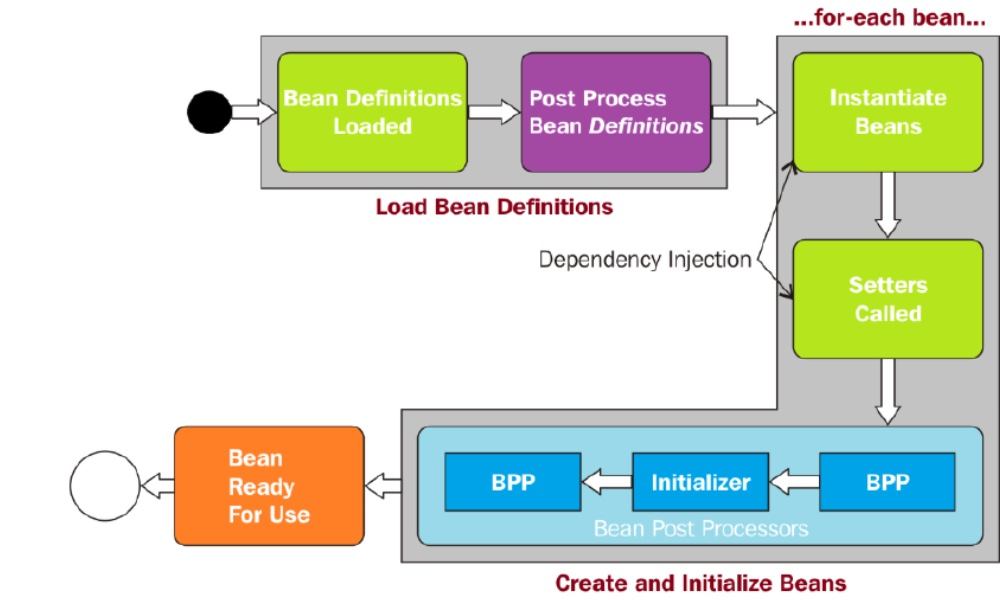
\includegraphics[width=1\linewidth]{bean-lifecycle-3}
    \caption{Lifecycle overview}
    \label{fig:bean-lifecycle-3}
\end{figure}

Figure \ref{fig:bean-lifecycle-2} focuses on pre-initialization.

\begin{figure}
    \centering
    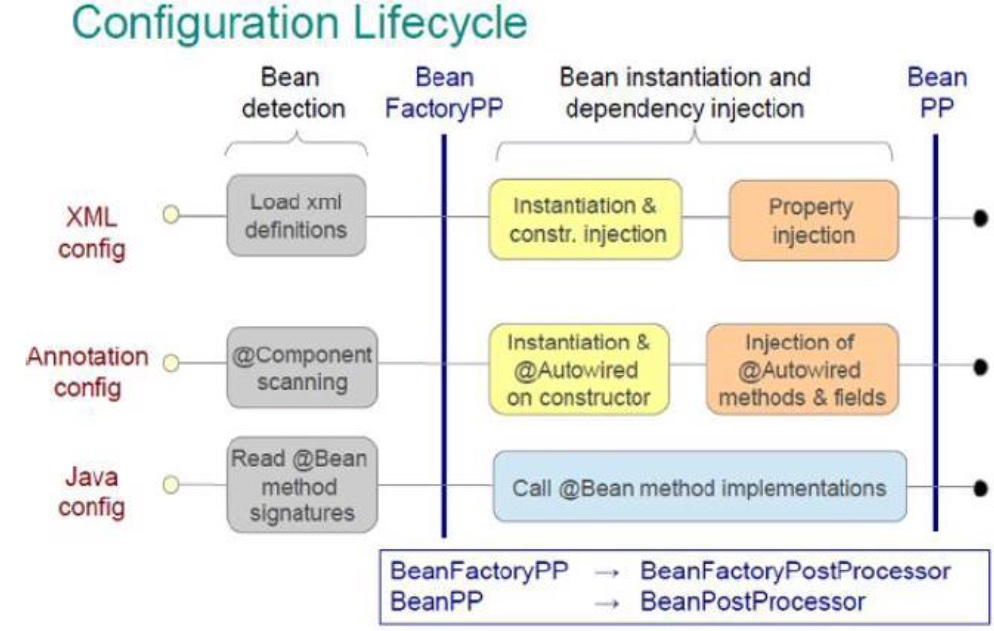
\includegraphics[width=1\linewidth]{bean-lifecycle-2}
    \caption{Zooming in on pre-instantiation}
    \label{fig:bean-lifecycle-2}
\end{figure}

On the other hand, fig. \ref{fig:bean-lifecycle-1} zooms in on post-instantiation.

\begin{figure}
    \centering
    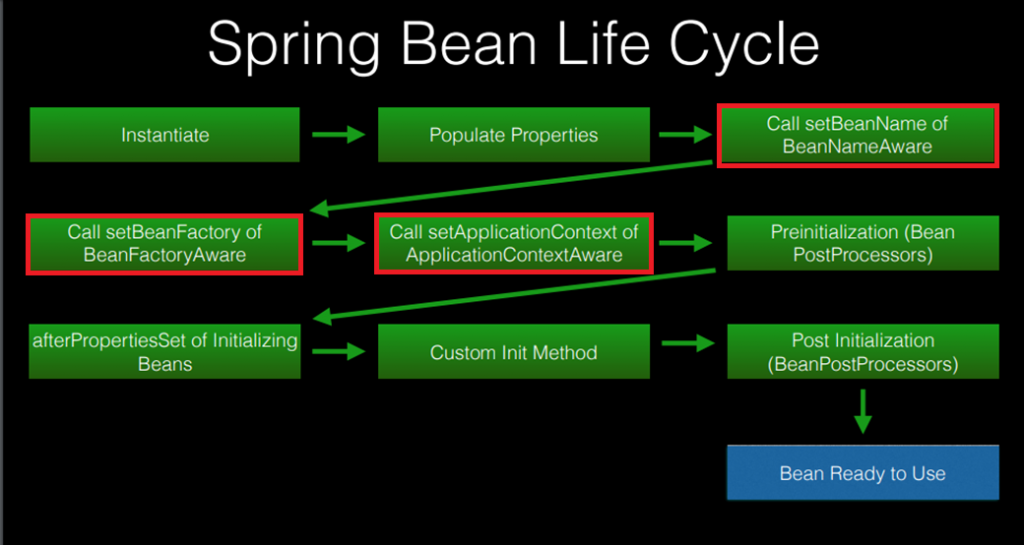
\includegraphics[width=1\linewidth]{bean-lifecycle-1}
    \caption{Zooming in on post-instantiation}
    \label{fig:bean-lifecycle-1}
\end{figure}


See https://www.digitalocean.com/community/tutorials/spring-bean-life-cycle for code to display the order of invocations.

\subsubsection{Load bean definitions, creating an ordered graph}
In this step, all the configuration files – @Configuration classes or XML files – are processed. For annotation-based configuration, all the classes annotated with @Components are scanned to load the bean definitions.

Bean definitions are passed to a BeanFactory, each under its id and type. For example, ApplicationContext is a BeanFactory.

Then, BeanFactoryPostProcessors are run.

\subsubsection{Instantiate and run BeanFactoryPostProcessors}
In a Spring application, a BeanFactoryPostProcessor can modify the definition of any bean.
The BeanFactory object is passed as an argument to the postProcess() method of the BeanFactoryPostProcessor. BeanFactoryPostProcessor then works on the bean definitions or the configuration metadata of the bean before the beans are actually created.
Spring provides several useful implementations of BeanFactoryPostProcessor, such as reading properties and registering a custom scope. We can write our own implementation of the BeanFactoryPostProcessor interface. To influence the order in which bean factory post processors are invoked, their bean definition methods may be annotated with the @Order annotation. If you are implementing your own bean factory post processor, the implementation class can also implement the Ordered interface.

\begin{figure}
    \centering
    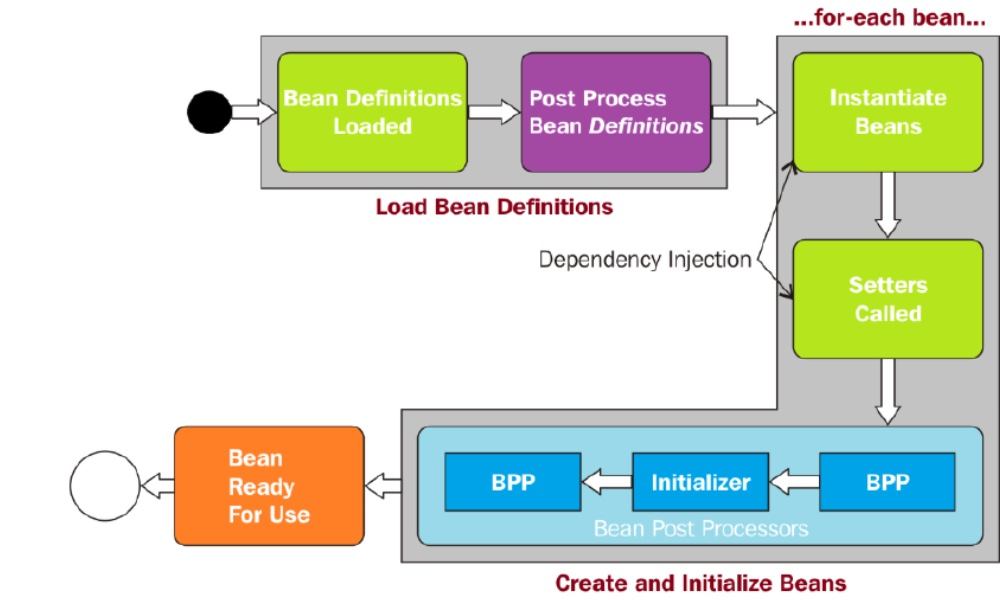
\includegraphics[width=1\linewidth]{bean-lifecycle-3}
    \caption{}
    \label{fig:bean-lifecycle-1}
\end{figure}

\subsubsection{Instantiate beans}
Injects values and bean references into beans’ properties.

\subsubsection{Call BeanNameAware’s setBeanName() for each bean implementing it}

\subsubsection{Call BeanFactoryAware’s setBeanFactory() passing the bean factory for each bean implementing it}

\subsubsection{Call ApplicationContextAware’s setApplicationContext for each bean implementing it}

\subsubsection{Before initialization: Run pre-initialization BeanPostProcessors}
The Application context calls postProcessBeforeInitialization() for each bean implementing BeanPostProcessor.

\begin{lstlisting}
    public interface BeanPostProcessor {

        /**
        * Apply this {@code BeanPostProcessor} to the given new bean instance before any bean's initialization callbacks (like InitializingBean's afterPropertiesSet
        * or a custom init-method).
        **/
        @Nullable
        default Object postProcessBeforeInitialization(Object bean, String beanName) throws BeansException {
            return bean;
        }

        /**
        * Apply this {@code BeanPostProcessor} to the given new bean instance after any bean initialization callbacks (like InitializingBean's afterPropertiesSet
        * or a custom init-method).
        */
        @Nullable
        default Object postProcessAfterInitialization(Object bean, String beanName) throws BeansException {
            return bean;
        }
    }
\end{lstlisting}

In postProcessBeforeInitialization and postProcessAfterInitialization, a bean implementing BeanPostProcessor can return anything it wants - even something completely different!

Figure \ref{fig:custom_bean_postprocessor} shows a no-op implementation.

\begin{figure}
    \centering
    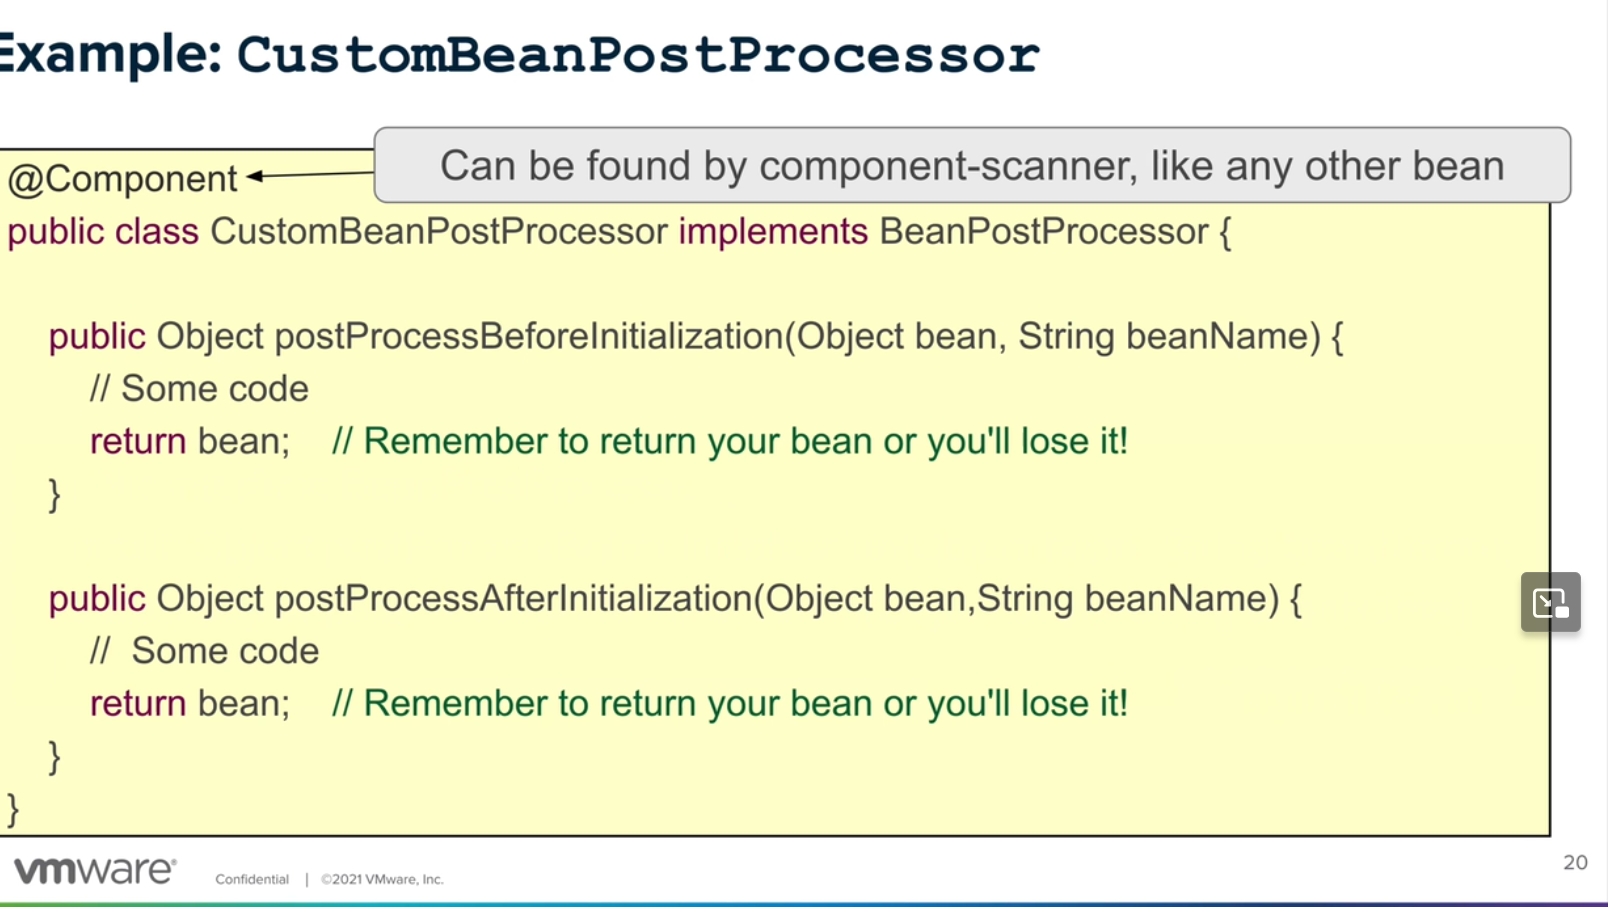
\includegraphics[width=1\linewidth]{custom_bean_postprocessor}
    \caption{Custom bean postprocessor}
    \label{fig:custom_bean_postprocessor}
\end{figure}

\subsubsection{Initialization hook 1: JSR 250's \lstinline|@PostConstruct|}

Of the three ways to tune in to Spring's lifecycle events, the first method called is JSR 250's @PostConstruct annotation.

Example:

\begin{lstlisting}
    @PostConstruct
    public void init(){
        System.out.println("MyService init method called");
    }
\end{lstlisting}

\lstinline|@PostConstruct| (as well as \lstinline|init-method|) is enabled by Spring's  \lstinline|CommonAnnotationBeanPostProcessor|. This is a
BeanPostProcessor implementation that supports common Java annotations out of the box, in particular the JSR-250 annotations in the javax.annotation package.

It includes support for the javax.annotation.PostConstruct and javax.annotation.PreDestroy annotations - as init annotation and destroy annotation, respectively - through inheriting from InitDestroyAnnotationBeanPostProcessor with pre-configured annotation types.

\begin{lstlisting}
    public class CommonAnnotationBeanPostProcessor extends InitDestroyAnnotationBeanPostProcessor
    implements InstantiationAwareBeanPostProcessor, BeanFactoryAware, Serializable {...}

\end{lstlisting}

\subsubsection{Initialization hook 2: \lstinline|InitializingBean|’s \lstinline|afterPropertiesSet()|}
If a bean implements the InitializingBean interface, Spring calls its afterPropertiesSet() method. Used to initialize processes,  load resources, etc. This approach is simple to use but it’s not recommended because it will create tight coupling with the Spring framework in our bean implementations.

\begin{lstlisting}
    public interface InitializingBean {

        /**
        * Invoked by the containing BeanFactory after it has set all bean properties.
        * This method allows the bean instance to perform validation of its overall configuration and final initialization when all bean properties have been set.
        */
        void afterPropertiesSet() throws Exception;

    }
\end{lstlisting}

\subsubsection{Initialization hook 3: \lstinline|Init-Method|}
As last of the three, the init-method of the bean tag (the initMethod attribute of the @Bean annotation, respectively) is called.

Here we use the init-method attribute:

\begin{lstlisting}
    <bean name="myEmployeeService" class="com.journaldev.spring.service.MyEmployeeService"
    init-method="init" destroy-method="destroy">
    <property name="employee" ref="employee"></property>
    </bean>
\end{lstlisting}

Using init-method is a solution when you don't own the class (and so, can't annotate it).

\subsubsection{Bean ready to use}
Your beans remain live in the application context until it is closed by calling the close() method of the application context.

\subsubsection{Custom destruction}
If a bean implements the DisposableBean interface, Spring calls its destroy() method to destroy any process or clean up the resources of your application. There are other methods to achieve this step-for example, you can use the destroy-method of the tag, the destroyMethod attribute of the `@Bean` annotation, and JSR 250's `@PreDestroy` annotation.

Precisely, the order of invocation is this:

\begin{itemize}
    \item Any methods in the bean implementation class annotated with @PreDestroy are invoked.
    \item Any destroy method in a bean implementing the DisposableBean interface is invoked.
    \item Any custom bean destruction method is invoked. Bean destruction methods can be specified either in the value of the destroy-method attribute in the corresponding \textless bean \textgreater element in a Spring XML configuration or in the destroyMethod property of the @Bean annotation.
\end{itemize}

\subsection{Customizing the Nature of a Bean}
\subsubsection{Lifecycle Callbacks}

To interact with the container’s management of the bean lifecycle, you can implement the Spring
\lstinline|| and \lstinline|DisposableBean| interfaces. The container calls \lstinline|afterPropertiesSet()| for the
former and \lstinline|destroy()| for the latter to let the bean perform certain actions upon initialization and
destruction of your beans.

The JSR-250 \lstinline|@PostConstruct| and \lstinline|@PreDestroy| annotations are generally considered
best practice for receiving lifecycle callbacks in a modern Spring application. Using these annotations means that your beans are not coupled to Spring-specific
interfaces.

If you do not want to use the JSR-250 annotations but you still want to remove
coupling, consider init-method and destroy-method bean definition metadata.

Multiple lifecycle mechanisms configured for the same bean, with different initialization methods,
are called as follows:

\begin{enumerate}
    \item Methods annotated with @PostConstruct
    \item afterPropertiesSet() as defined by the InitializingBean callback interface
    \item A custom configured init() method
\end{enumerate}

Destroy methods are called in the same order:

\begin{enumerate}
    \item Methods annotated with @PreDestroy
    \item destroy() as defined by the DisposableBean callback interface
    \item A custom configured destroy() method
\end{enumerate}

Internally, the Spring Framework uses \lstinline|BeanPostProcessor| implementations to process any callback
interfaces it can find and call the appropriate methods. If you need custom features or other
lifecycle behavior Spring does not by default offer, you can implement a BeanPostProcessor yourself.


\subsubsection{Listenening to Application Context startup/shutdown}

In addition to the individual bean initialization and destruction callbacks, Spring-managed objects may also
implement the \lstinline|Lifecycle| interface so that those objects can participate in the startup and shutdown
process, as driven by the container’s own lifecycle.

The Lifecycle interface defines the essential methods for any object that has its own lifecycle requirements (such as starting and stopping some background process):

\begin{lstlisting}
    public interface Lifecycle {
        void start();
        void stop();
        boolean isRunning();
    }
\end{lstlisting}

Any Spring-managed object may implement the Lifecycle interface.
Then, when the ApplicationContext itself receives start and stop signals (for example, for a stop/restart scenario at runtime), it cascades those calls to all Lifecycle implementations defined within that context. It
does this by delegating to a LifecycleProcessor, shown in the following listing:

\begin{lstlisting}
    public interface LifecycleProcessor extends Lifecycle {
        void onRefresh();
        void onClose();
    }
\end{lstlisting}

Notice that the LifecycleProcessor is itself an extension of the Lifecycle interface. It also adds two
other methods for reacting to the context being refreshed and closed.

\subsubsection{Aware Interfaces}

Indicates that the bean is eligible to be notified by the Spring container through the callback methods.
A typical use case for BeanNameAware could be acquiring the bean name for logging or wiring purposes. For the BeanFactoryAware it could be the ability to use a spring bean from legacy code.
In most cases, we should avoid using any of the Aware interfaces, unless we need them. Implementing these interfaces will couple the code to the Spring framework.

\paragraph{BeanNameAware}

Makes the object aware of the bean name defined in the container.

\begin{lstlisting}
    public class MyBeanName implements BeanNameAware {
        @Override
        public void setBeanName(String beanName) {
            System.out.println(beanName);
        }
    }
    @Configuration
    public class Config {
        @Bean(name = "myCustomBeanName")
        public MyBeanName getMyBeanName() {
            return new MyBeanName();
        }
    }
    AnnotationConfigApplicationContext context
    = new AnnotationConfigApplicationContext(Config.class);
    MyBeanName myBeanName = context.getBean(MyBeanName.class);

\end{lstlisting}

\paragraph{BeanFactoryAware}

Provides access to the BeanFactory which created the object.

\begin{lstlisting}
    public class MyBeanFactory implements BeanFactoryAware {
        private BeanFactory beanFactory;
        @Override
        public void setBeanFactory(BeanFactory beanFactory) throws BeansException {
            this.beanFactory = beanFactory;
        }
        public void getMyBeanName() {
            MyBeanName myBeanName = beanFactory.getBean(MyBeanName.class);
            System.out.println(beanFactory.isSingleton("myCustomBeanName"));
        }
    }
    MyBeanFactory myBeanFactory = context.getBean(MyBeanFactory.class);
    myBeanFactory.getMyBeanName();}
    \end{lstlisting}

    \paragraph{ApplicationContextAware}
    \begin{lstlisting}
public class ApplicationContextAwareImpl implements ApplicationContextAware {
    @Override
    public void setApplicationContext(ApplicationContext applicationContext) throws BeansException {
        User user = (User) applicationContext.getBean("user");
        System.out.println("User Id: " + user.getUserId() + " User Name :" + user.getName());}}
        \end{lstlisting}

\subsubsection{Customizing Beans by Using a BeanPostProcessor}

\subsubsection{Customizing Configuration Metadata with a BeanFactoryPostProcessor}

\subsubsection{Customizing Instantiation Logic with a FactoryBean}

\section{Annotations}
\subsection{Annotations for dependency injection}
\subsubsection{@Autowired}
    @Autowired marks a dependency which Spring is going to resolve and inject. We can use this annotation with constructor, setter, or field injection. E.g.,

    \begin{lstlisting}
        class Car {
            @Autowired
            Engine engine;
        }
    \end{lstlisting}

    Starting with version 4.3, we don’t need to annotate constructors with @Autowired explicitly unless we declare at least two constructors.

    @Autowired matches by type. If there are several classes matching the required type (e.g., implementing the same interface), @Autowired needs to be supplemented by @Qualifier:

    \begin{lstlisting}
        @Component("Repo1")
        class Repo1 implements Repo {}

        @Component("Repo2")
        class Repo2 implements Repo {}

        @Component
        public class Service1 implements ServiceX {
            public Service1(@Qualifier("Repo2") Repo){}

        }

    \end{lstlisting}

    If there is no @Qualifier given, @Autowired looks for a bean annotated with @Primary. If none exists, Spring will match by bean name ( = bean id).

    Here, Spring will look for a bean named x:

    \begin{lstlisting}
        // constructor injection
        @Autowired
        public MyBean(X x){}

       // method injection
       @Autowired
       public setX(X x){}

       // field injection
       @Autowired
       private X x;
    \end{lstlisting}

\subsubsection{Using @Primary in conjunction with @Qualified}

For example, when you work with two different databases, using the @Primary annotation allows you to specify the main DataSource. Additional DataSources can be configured with different qualifiers, allowing you to inject them as needed.

\begin{lstlisting}

    @Configuration
    public class DataSourceConfig {

        @Bean
        @Primary
        @ConfigurationProperties(prefix = "spring.datasource")
        public DataSource primaryDataSource() {
            return DataSourceBuilder.create().build();
        }

        @Bean
        @ConfigurationProperties(prefix = "spring.second-datasource")
        public DataSource secondaryDataSource() {
            return DataSourceBuilder.create().build();
        }
    }

\end{{lstlisting}

\subsubsection{@Bean}

    @Bean marks a factory method which instantiates a Spring bean.

    \begin{lstlisting}
        @Bean
        Engine engine() {
            return new Engine();
        }
    \end{lstlisting}

    Spring calls these methods when a new instance of the return type is required. All methods annotated with @Bean must be in @Configuration classes.


\subsubsection{@Resource}

The @Resource annotation matches by name, type, or qualifier (in this order). It is applicable to setter and field injection.
Here’s an example injecting a field. Note that the bean id and the corresponding reference attribute value must match:

\begin{lstlisting}
    @Configuration
    public class MyAppContext {
        @Bean(name="namedFile")
        public File namedFile() {
            File namedFile = new File("namedFile.txt");
            return namedFile;
        }
    }

    @ContextConfiguration(
    loader=AnnotationConfigContextLoader.class,
    classes= MyAppContext.class)
    public class Xxx {
        @Resource(name="namedFile")
        private File defaultFile;
    }
\end{lstlisting}

\subsubsection{@Inject and @Named}

Spring offers support for JSR-330 standard annotations (Dependency Injection). Those annotations are scanned in the same way as the Spring annotations. To use them, you need to have the relevant jars in your classpath.

The @Inject annotation matches by type, qualifier, or name (in this order). It is applicable to setter and field injection. With @Inject, the class reference variable's name and the bean name don’t have to match.

To use the @Inject annotation, declare the javax.inject library as a Gradle or Maven dependency.

\begin{lstlisting}
    public class MyAppContext {
        @Bean
        // no bean name specified - method name is used
        public File getSomeFile() {
            File namedFile = new File("namedFile.txt");
            return namedFile;
        }
    }

    @ContextConfiguration(
    loader=AnnotationConfigContextLoader.class,
    classes= MyAppContext.class)
    public class Xxx {
        @Inject
        private File defaultFile;
    }
\end{lstlisting}

Furthermore, you may declare your injection point as a Provider, allowing for on-demand access to beans of shorter scopes or lazy access to other beans through a Provider.get() call. The following example offers a variant of the preceding example:

\begin{lstlisting}
    import jakarta.inject.Inject;
    import jakarta.inject.Provider;

    public class SimpleMovieLister {

        private Provider<MovieFinder> movieFinder;

        @Inject
        public void setMovieFinder(Provider<MovieFinder> movieFinder) {
            this.movieFinder = movieFinder;
        }

    public void listMovies() {
        this.movieFinder.get().findMovies(...);
        // ...
    }
}
\end{lstlisting}

If you would like to use a qualified name for the dependency that should be injected, you should use the\lstinline| @Named| annotation, as the following example shows:

\begin{lstlisting}
    import jakarta.inject.Inject;
    import jakarta.inject.Named;

    public class SimpleMovieLister {

        private MovieFinder movieFinder;

        @Inject
        public void setMovieFinder(@Named("main") MovieFinder movieFinder) {
            this.movieFinder = movieFinder;
        }

        // ...
    }
\end{lstlisting}

\subsubsection{@Named and @ManagedBean: Standard Equivalents to the @Component Annotation}

Instead of @Component, you can use @jakarta.inject.Named or jakarta.annotation.ManagedBean:

\begin{lstlisting}

import jakarta.inject.Inject;
import jakarta.inject.Named;

@Named("movieListener")  // @ManagedBean("movieListener") could be used as well
public class SimpleMovieLister {

    private MovieFinder movieFinder;

    @Inject
    public void setMovieFinder(MovieFinder movieFinder) {
        this.movieFinder = movieFinder;
    }

    // ...
}
\end{lstlisting}

It is very common to use @Component without specifying a name for the component. @Named can be used in a similar fashion:

\begin{lstlisting}
    import jakarta.inject.Inject;
    import jakarta.inject.Named;

    @Named
    public class SimpleMovieLister {

        private MovieFinder movieFinder;

        @Inject
        public void setMovieFinder(MovieFinder movieFinder) {
            this.movieFinder = movieFinder;
        }

        // ...
    }
\end{lstlisting}

When you use @Named or @ManagedBean, you can use component scanning in the exact same way as when you use Spring annotations:

\begin{lstlisting}

@Configuration
@ComponentScan(basePackages = "org.example")
public class AppConfig  {
    // ...
}

\end{lstlisting}
I

\subsubsection{@Value}

    We can use @Value for injecting property values into beans. It’s compatible with constructor, setter, and field injection. E.g.,

    \begin{lstlisting}
        Engine(@Value("8") int cylinderCount) {
            this.cylinderCount = cylinderCount;
        }
    \end{lstlisting}

    This is an alternative to making explicit use of Spring's Environment bean. E.g.

    \begin{lstlisting}
       public DataSource dataSource(
        @Value("${db.driver}") String driver,
        ...
        )
        }
    \end{lstlisting}

\subsubsection{@DependsOn}

    We can use this annotation to make Spring initialize other beans before the annotated one. Usually, this behavior is automatic, based on the explicit dependencies between beans. We only need this annotation when the dependencies are implicit, for example, JDBC driver loading or static variable initialization. E.g.,

     \begin{lstlisting}
        @Bean
        @DependsOn("fuel")
        Engine engine() {
            return new Engine();
        }
    \end{lstlisting}

\subsubsection{@Lazy}

    This annotation behaves differently depending on where exactly we place it.

    \begin{itemize}
        \item In an @Bean-annotated bean factory method, it is used to delay the method call (hence the bean creation)
        \item With an @Configuration class, all contained @Bean methods will be affected
        \item For all other @Component classes,  they will be initialized lazily when so annotated.
        \item @Autowired constructors, setters, and fields will be loaded lazily (via proxy).
    \end{itemize}

    \begin{lstlisting}
        @Configuration
        @Lazy
        class VehicleFactoryConfig {

            @Bean
            @Lazy(false)
            Engine engine() {
                return new Engine();
            }
        }
    \end{lstlisting}

\subsubsection{@Scope}

   The Spring Framework supports six scopes, four of which are available only if you use a web-aware ApplicationContext. You can also create a custom scope.

   These are:

   \begin{itemize}
       \item singleton
       \item    prototype
       \item    request
       \item    session
       \item    application: Scopes a single bean definition to the lifecycle of a ServletContext.
       \item    websocket
   \end{itemize}

\subsection{Context Configuration Annotations}

\subsubsection{@Import}

    With @import, we can use specific @Configuration classes without component scanning.

    \begin{lstlisting}
        @Import(VehiclePartSupplier.class)
        class VehicleFactoryConfig {}

        // use array to import several classes
        @Import({Demo1.class, Demo2.class})
    \end{lstlisting}

\subsubsection{@ImportResource}

    We can import XML configurations with @ImportResource. We can specify the XML file locations with the locations argument, or with its alias, the value argument:

    \begin{lstlisting}
        @Configuration
        @ImportResource("classpath:/annotations.xml")
        class VehicleFactoryConfig {}
    \end{lstlisting}

\subsubsection{@PropertySource}

    With this annotation, we set properties using a POJO.

    \begin{lstlisting}
        @Configuration
        @PropertySource("classpath:/annotations.properties")
        @PropertySource("classpath:/vehicle-factory.properties")
        class VehicleFactoryConfig {}
    \end{lstlisting}

    These properties can be used by Spring's Environment bean, in addition to environment variables and Java system properties.

    Allowed prefixes are classpath:, file:, and http:.

\subsection{Bean annotations}

\subsubsection{@Profile}

    Profiles are a way to group bean definitions, for example:

     \begin{itemize}
        \item dev, test, prod environment
        \item jdbc, jpa [implementations]
    \end{itemize}

   The @Profile annotation may be used in any of the following ways:

   \begin{itemize}
       \item At class level in @Configuration classes.
       \item At class level in classes annotated with @Component or annotated with any other annotation that in turn is annotated with @Component.
       \item On methods annotated with the @Bean annotation.
   \end{itemize}

    The profile string may contain a simple profile name (for example, production) or a profile expression. A profile expression allows for more complicated profile logic to be expressed. The following operators are supported in profile expressions: \lstinline{!,\&,|}.

    To define alternative beans with different profile conditions, use distinct Java method names pointing to the same bean name via the @Bean name attribute:

    \begin{lstlisting}
        @Bean("dataSource")
        @Profile("development")
        public DataSource standaloneDataSource(){

        @Bean("dataSource")
        @Profile("production")
        public DataSource jndiDataSource() throws Exception {}

    \end{lstlisting}

   Spring uses two separate properties when determining which profiles are active, spring.profiles.active and spring.profiles.default:

    \begin{itemize}
       \item If spring.profiles.active is set,  then its value determines which profiles are active.
       \item If spring.profiles.active isn’t set, then Spring looks to spring.profiles.default.
       \item If neither spring.profiles.active nor spring.profiles.default is set, only those beans that aren’t defined as being in a profile are created.
    \end{itemize}

   These properties can be set on the command line:

   \begin{lstlisting}[language=bash]
       -Dspring.profiles.active=embedded.jpa
   \end{lstlisting}

   , programmatically:

   \begin{lstlisting}
       System.setProperty("spring.profiles.active", "embedded.jpa");
   \end{lstlisting}

   , or via an annotation (@ActiveProfiles; integration tests only).

\subsubsection{Conditional}

Indicates that a component is only eligible for registration when all specified conditions match.

The @Conditional annotation may be used in any of the following ways:

\begin{itemize}
    \item as a type-level annotation on any class directly or indirectly annotated with @Component, including @Configuration classes
    \item as a meta-annotation, for the purpose of composing custom stereotype annotations
    \item as a method-level annotation on any @Bean method
\end{itemize}

If a @Configuration class is marked with @Conditional, all of the @Bean methods, @Import annotations, and @ComponentScan annotations associated with that class will be subject to the conditions.

\subsubsection{@ComponentScan}

    The @ComponentScan annotation is used together with @Configuration.

    @ComponentScan can be used with and without arguments.

    Without arguments, @ComponentScan  tells Spring to scan the current package and all of its sub-packages.

    With arguments, @ComponentScan tells which packages or classes to scan. E.g., specifying packages:

    \begin{lstlisting}
        @Configuration
        @ComponentScan(basePackages = "com.baeldung.annotations")
        class VehicleFactoryConfig {}
    \end{lstlisting}

    Or else, specifying classes:

    \begin{lstlisting}
        @Configuration
        @ComponentScan(basePackageClasses = VehicleFactoryConfig.class)
        class VehicleFactoryConfig {}
    \end{lstlisting}

    We can specify multiple package names, using spaces, commas, or semicolons as a separator.

    \begin{lstlisting}
        @ComponentScan(basePackages = "springapp.animals;springapp.flowers")
        @ComponentScan(basePackages = "animals,springapp.flowers")
        @ComponentScan(basePackages = "springapp.animals springapp.flowers")
    \end{lstlisting}

    We could also apply a filter, choosing from a range of filter types. For example:

    \begin{lstlisting}
        @ComponentScan(excludeFilters =
        @ComponentScan.Filter(type=FilterType.REGEX,
        pattern="com\\.baeldung\\.componentscan\\.springapp\\.flowers\\..*"))
    \end{lstlisting}

    Or:
    \begin{lstlisting}
        @ComponentScan(excludeFilters =
        @ComponentScan.Filter(type = FilterType.ASSIGNABLE\_TYPE, value = Rose.class))
    \end{lstlisting}

\subsubsection{@Component}

    @Component is a class-level annotation. During component scan, Spring automatically detects classes annotated with @Component.

    \begin{lstlisting}
        @Component
        class CarUtility {
            // ...
        }
    \end{lstlisting}

    @Repository, @Service, @Configuration, and @Controller are all meta-annotations of (i.e., themselves annotated with) @Component. E.g.,

      \begin{lstlisting}
        @Component
        public @interface Service {}
    \end{lstlisting}

    Spring also automatically picks them up during the component scanning process.


\subsubsection{@Repository}

    \begin{lstlisting}
        @Repository
        class VehicleRepository {
            // ...
        }
    \end{lstlisting}

\subsubsection{@Service}

    \begin{lstlisting}
        @Service
        public class VehicleService {
            // ...
        }
    \end{lstlisting}

\subsubsection{@Controller}

    \begin{lstlisting}
        @Controller
        public class VehicleController {
            // ...
        }
    \end{lstlisting}

\subsubsection{@Configuration}

    Configuration classes can contain bean definition methods annotated with @Bean.

    \begin{lstlisting}
        @Configuration
        class VehicleFactoryConfig {

            @Bean
            Engine engine() {
                return new Engine();
            }

        }
    \end{lstlisting}

\subsubsection{@JdkProxyHint}

In Spring Boot 2.5, the @JdkProxyHint annotation was introduced to address compatibility issues with GraalVM's native image generation. GraalVM is a high-performance runtime that can compile Java applications into native executables, providing improved startup time and reduced memory footprint.

When using Spring Boot with GraalVM native image generation, the default dynamic proxy mechanism based on JDK proxies may cause issues. The @JdkProxyHint annotation allows developers to configure specific beans or bean types to be processed differently when generating the native image. By providing hints, Spring Boot can switch to alternative proxying mechanisms, such as CGLIB proxies, to ensure compatibility with GraalVM.

\subsection{Spring MVC annotations}

\subsubsection{@RequestMapping}

This annotation can be used both at the class and at the method level.

In most cases, at the method level applications will prefer to use one of the HTTP method specific variants @GetMapping, @PostMapping, @PutMapping, @DeleteMapping, or @PatchMapping.

Example, passing the path and the method (all optional):

\begin{lstlisting}
    @RequestMapping(path="/profile", method = RequestMethod.PUT)
\end{lstlisting}

\subsection{Spring Boot Annotations}
\subsubsection{@SpringBootApplication}

    This is a combination of three annotations:

    \begin{lstlisting}
        // enable registration of extra beans in the context or the import of additional configuration classes. An alternative to Spring's standard @Configuration that aids configuration detection in your integration tests.
        @SpringBootConfiguration
        @EnableAutoConfiguration
        @ComponentScan
    \end{lstlisting}

 Here is its definition:

    \begin{lstlisting}
        @Target(TYPE)
        @Retention(RUNTIME)
        @Documented
        @Inherited
        @SpringBootConfiguration
        @EnableAutoConfiguration
        @ComponentScan(excludeFilters={@Filter(
            type=CUSTOM,
            classes=TypeExcludeFilter.class),})
        public @interface SpringBootApplication

    \end{lstlisting}

\subsubsection{@ConfigurationProperties}

    Helps keep configuration clean (see \ref{fig:configurationproperties}).

    This annotation has to be enabled via one of:
    \begin{itemize}
        \item @EnableConfigurationProperties on the application class

        \begin{lstlisting}
         @SpringBootApplication
         @EnableConfigurationProperties(
            ConnectionSettings.class)
         public class App {
             // ...
         }
        \end{lstlisting}

        \item @ConfigurationPropertiesScan  on the application class

        \begin{lstlisting}
         @SpringBootApplication
         @ConfigurationPropertiesScan
         public class App {
             // ...
         }
        \end{lstlisting}

        \item @Component on the configuration class

        \begin{lstlisting}
         @Component
         @ConfigurationProperties(prefix="...")
         public class ConnectionSettings {
             // ...
         }
        \end{lstlisting}

    \end{itemize}

\begin{figure}
    \centering
    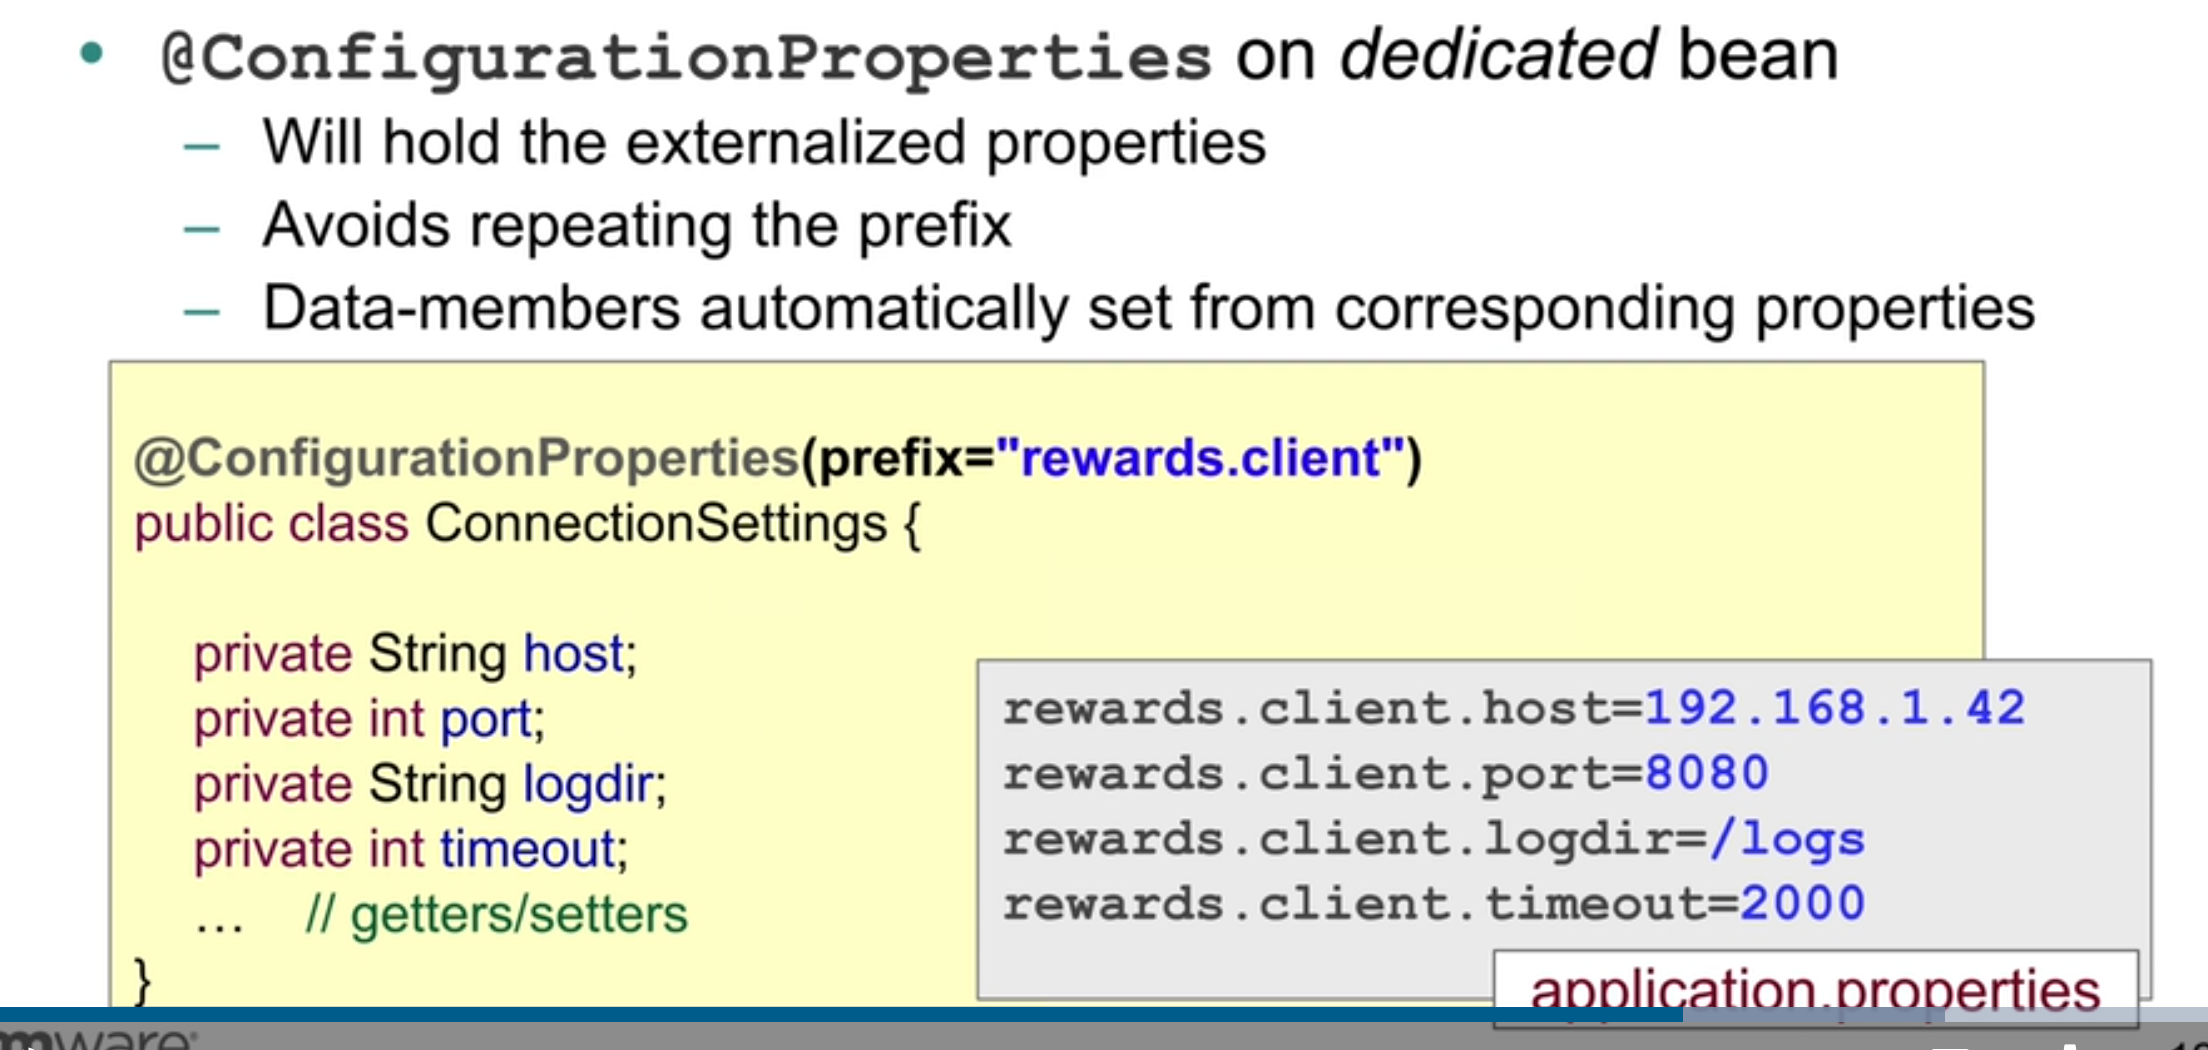
\includegraphics[width=1\linewidth]{configurationproperties}
    \caption{}
    \label{fig:configurationproperties}
\end{figure}

\subsubsection{@ConditionalOnX}

Determine what auto configuration does. There are:

\begin{lstlisting}
    ConditionalOnBean
    ConditionalOnSingleCandidate
    onditionalOnMissingBean

    ConditionalOnCheckpointRestore

    ConditionalOnClass
    ConditionalOnMissingClass

    ConditionalOnCloudPlatform

    //  allows conditional auto-configuration based on the evaluation of a SpEL expression.
    ConditionalOnExpression

    // @Conditional that matches based on the JVM version the application is running on.
    ConditionalOnJava
    ConditionalOnJava.Range

    ConditionalOnJndi

    ConditionalOnWarDeployment
    ConditionalOnNotWarDeployment

    ConditionalOnWebApplication
    ConditionalOnWebApplication.Type
    ConditionalOnNotWebApplication

    // @Conditional that checks if the specified properties have a specific value.
    ConditionalOnProperty

    // @Conditional that only matches when the specified resources are on the classpath.
    ConditionalOnResource

    ConditionalOnThreading

\end{lstlisting}



For example, @Profile is such a condition.

\subsubsection{RestController}

Includes @Controller and @ResponseBody.

\begin{figure}
    \centering
    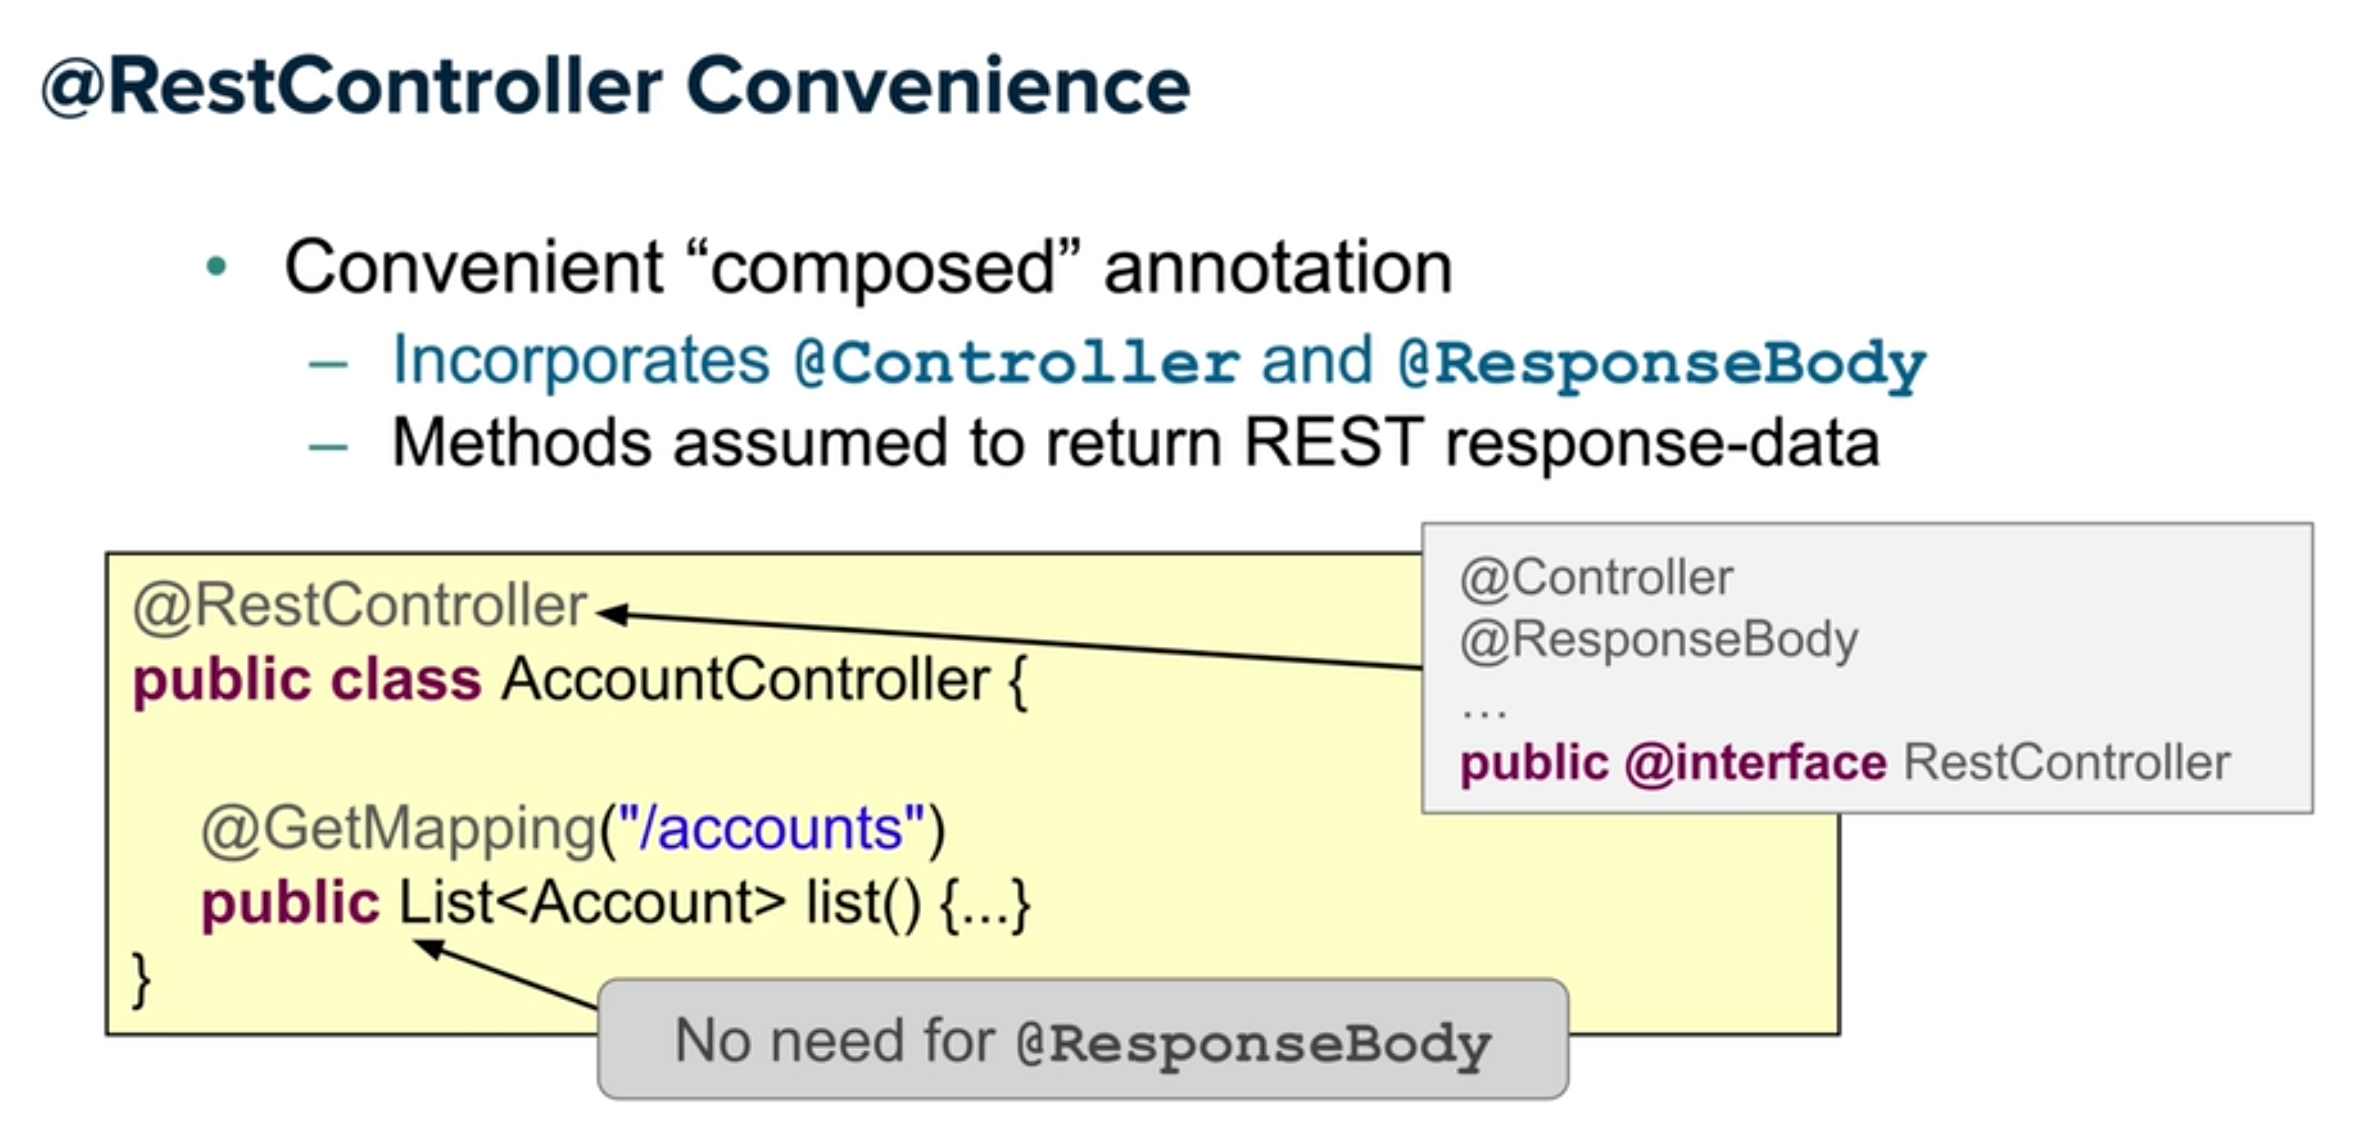
\includegraphics[width=1\linewidth]{restcontroller}
    \caption{RestController convenience annotation.}
    \label{fig:restcontroller}
\end{figure}

\subsubsection{Request URI Decomposition: @RequestParam, @PathVariable}

Do implicit type conversion of arguments.

\begin{lstlisting}
    // localhost:8080/account?userid=12345
    @GetMapping("/account")
    public List<Account> list(@RequestParam("userid"} int userid) {}

    // localhost:8080/accounts/12345
    @GetMapping("/accounts/{accountId}")
    public Account find (@PathVariable("accountId"} long id) {}

    // if argument name is missing, will take from the mapping
    // could also have

    // localhost:8080/account?overdrawn=12345
    @GetMapping("/account")
    public List<Account> list(@RequestParam int overdrawn) {}

    // localhost:8080/accounts/12345
    @GetMapping("/accounts/{accountId}")
    public Account find (@PathVariable long id) {}

    // localhost:8080/accounts/12345?overdrawn=true
    @GetMapping("/accounts/{accountId}")
    public Account find (
        @PathVariable long accountId,
        @RequestParam boolean overdrawn
    ) {}



\end{lstlisting}

\subsubsection{@ResponseBody}

Causes Java objects returned by the Controller to be processed by HttpMessageConverters in order to return information to the client in the form requested in the Accept header.

Example (assuming the client requests JSON):

Here, the @ResponseBody annotation tells a controller that the \textit{object} returned is automatically serialized into \textit{JSON} and passed back into the \textit{HttpResponse} object.

Suppose we have a custom Response object:

\begin{lstlisting}
    public class ResponseTransfer {
        private String text;

        // standard getters/setters
    }
\end{lstlisting}

Next, the associated controller can be implemented:

\begin{lstlisting}
   @Controller
   @RequestMapping("/post")
   public class ExamplePostController {

       @Autowired
       ExampleService exampleService;

       @PostMapping("/response")
       @ResponseBody
       public ResponseTransfer postResponseController(
       @RequestBody LoginForm loginForm) {
           return new ResponseTransfer("Thanks For Posting!!!");
       }
   }
\end{lstlisting}

\subsubsection{@ResponseStatus}

    Used to return a status other than 200.

    \begin{lstlisting}
        @ResponseStatus(HttpStatus.NO_CONTENT)
        public void updateOrder(...){}
    \end{lstlisting}

\subsubsection{@RequestBody}

    Used to extract the request body.

    More precisely, @RequestBody maps the HttpRequest body to a transfer or domain object, enabling automatic deserialization of the inbound HttpRequest body onto a Java object.

    Example:

    \begin{lstlisting}

    @PostMapping("/request")
    public ResponseEntity postController(
    @RequestBody LoginForm loginForm) {

        exampleService.fakeAuthenticate(loginForm);
        return ResponseEntity.ok(HttpStatus.OK);
    }

    \end{lstlisting}
    Here, Spring automatically deserializes the JSON into a Java type, assuming an appropriate one is specified.

    \begin{lstlisting}
        @ResponseStatus(HttpStatus.NO_CONTENT)
        public void updateOrder(...){}
    \end{lstlisting}

    \begin{lstlisting}
        @ResponseStatus(HttpStatus.NO_CONTENT)
        public void updateOrder(...){}
    \end{lstlisting}


\section{Bean Naming}
\label{sec:bean-naming}
\subsection{Default Bean Naming}
\subsubsection{Class-level ("Annotation-based configuration")}
For an annotation used at the class level (@Component, @Service, @Controller), Spring uses the class name and converts the first letter to lowercase.
Custom names may be configured in the annotation's value attribute.

The type is determined from the annotated class, typically resulting in the actual
implementation class.

    \begin{lstlisting}
        @Service
        public class LoggingService { // bean name = loggingService

        }
    \end{lstlisting}

\subsubsection{Method-level ("Java configuration")}
When in a @Configuration class we use the @Bean annotation on a method, Spring uses the method name for the bean name.

    \begin{lstlisting}
        @Configuration
        public class AuditConfiguration {
            @Bean
            public AuditService audit() {
                return new AuditService();
            }
        }
    \end{lstlisting}

\subsection{Custom naming}

    \begin{lstlisting}
        @Component("myBean")
        public class MyCustomComponent {
        }
    \end{lstlisting}

   Custom names may be configured in @Bean's value attribute.

   The type is determined from the method return type, typically resulting in an interface.

\subsection{Naming Beans With @Bean and @Qualifier}
\subsubsection{@Bean With Value}
    The @Bean annotation is applied at the method level, and by default, Spring uses the method name as a bean name. We can override this using the @Bean annotation.

     \begin{lstlisting}
        @Configuration
        public class MyConfiguration {
            @Bean("beanComponent")
            public MyCustomComponent myComponent() {
                return new MyCustomComponent();
            }
        }
    \end{lstlisting}

\subsubsection{@Qualifier With Value}
    We can also use the @Qualifier annotation to name the bean.

    \begin{lstlisting}
        @Component
        @Qualifier("cat")
        public class Cat implements Animal {
            @Override
            public String name() {
                return "Cat";
            }
        }
        @Component
        @Qualifier("dog")
        public class Dog implements Animal {
            @Override
            public String name() {
                return "Dog";
            }
        }
        @Service
        public class PetShow {
            private final Animal dog;
            private final Animal cat;

            public PetShow (@Qualifier("dog")Animal dog, @Qualifier("cat")Animal cat) {
                this.dog = dog;
                this.cat = cat;
            }
            public Animal getDog() {
                return dog;
            }
            public Animal getCat() {
                return cat;
            }
        }
        \end{lstlisting}

\section{Spring Expression Language vs. Property Evaluation}

    Expressions in @Value annotations are of two types:

    \begin{itemize}
        \item Expressions starting with \$. Such expressions reference a property name in the application’s environment. These expressions are evaluated by the PropertySourcesPlaceholderConfigurer BeanFactoryPostProcessor prior to bean creation and can only be used in @Value annnotations.
        \item Expressions starting with \#.
        These expressions are parsed by a SpEL expression parser, and are evaluated by a SpEL expression instance.
    \end{itemize}

    In some cases, both can be used. For example, property values by default are Strings, but may be converted to primitives implicitly. So, both of these work:

    \begin{lstlisting}
        @Value("${daily.limit}")
        int limit;

        @Value("#{environment['daily.limit']}")
        int limit;
    \end{lstlisting}

    But if computations are to be performed, or object types are required, SpEL has to be used:

    \begin{lstlisting}
        // NO
        @Value("${daily.limit} * 2")

        // instead, do
        @Value("#{new Integer(environment['daily.limit']}) * 2")
    \end{lstlisting}

    To provide defaults, use a colon with property evaluation, and ?: in SpEL.

    \begin{lstlisting}
        @Value("${daily.limit}: 1000")
        int limit;

        @Value("#{environment['daily.limit']} ?: 1000")
        int limit;
    \end{lstlisting}

    In SpEL, Beans are referenced using @: e.g., \lstinline|@myComponent.toString()|.

    In addition to application-defined beans, SpEL can make use of beans implicitly provided by Spring, namely environment, systemProperties, and systemEnvironment.

\section{AOP in Spring}

\subsection{Core AOP Concepts}

\subsubsection{Join Point}

A point during the execution of a program, such as the execution of a method or the handling of an exception.

In Spring AOP, a join point always represents a method execution.


\subsubsection{Point Cut}

An expression that selects one or more join points.

Although Spring supports various AspectJ pointcut designators, the most commonly used one is \lstinline{execution}.

For this designator, the syntax pattern is as follows:

\begin{lstlisting}
    execution(
    modifiers-pattern?
    ret-type-pattern
    declaring-type-pattern.?name-pattern(param-pattern)
    throws-pattern?
    )
\end{lstlisting}

All parts except the returning type pattern (ret-type-pattern in the preceding snippet), the name pattern, and the parameters pattern are optional.

\begin{itemize}
    \item The returning type pattern determines what the return type of the method must be in order for a join point to be matched. * is most frequently used as the returning type pattern. It matches any return type. A fully-qualified type name matches only when the method returns the given type.
    \item  The name pattern matches the method name. You can use the * wildcard as all or part of a name pattern. If you specify a declaring type pattern, include a trailing . to join it to the name pattern component.
    \item The parameters pattern is slightly more complex: () matches a method that takes no parameters, whereas (..) matches any number (zero or more) of parameters. The (*) pattern matches a method that takes one parameter of any type. (*,String) matches a method that takes two parameters. The first can be of any type, while the second must be a String.

\end{itemize}

Examples:

\begin{lstlisting}
// The execution of any public method:
execution(public * *(..))

// The execution of any method with a name that begins with set:
execution(* set*(..))

// The execution of any method defined by the AccountService interface:
execution(* com.xyz.service.AccountService.*(..))

// The execution of any method defined in the service package:
execution(* com.xyz.service.*.*(..))

//The execution of any method defined in the service package or one of its sub-packages:
execution(* com.xyz.service..*.*(..))

// There is one directory between rewards and restaurant.
execution(* rewards.*.restaurant.*.*(..))

// There are 0 or more directories between rewards and restaurant.
execution(* rewards..restaurant.*.*(..))

// There must be at least 1 directory before restaurant.
// omitting the star is not allowed
execution(* *..restaurant.*.*(..))

// Any join point (method execution only in Spring AOP) within the service package:
within(com.xyz.service.*)

// Any join point (method execution only in Spring AOP) within the service package or one of its sub-packages:
within(com.xyz.service..*)

// Any join point (method execution only in Spring AOP) where the proxy implements the AccountService interface:
this(com.xyz.service.AccountService)

// Any join point (method execution only in Spring AOP) where the target object implements the AccountService interface:
target(com.xyz.service.AccountService)

// Any join point (method execution only in Spring AOP) that takes a single parameter and where the argument passed at runtime is Serializable.
// Note that the pointcut given in this example is different from execution(* *(java.io.Serializable)). The args version matches if the argument passed at runtime is Serializable, and the execution version matches if the method signature declares a single parameter of type Serializable.
args(java.io.Serializable)

// Any join point (method execution only in Spring AOP) where the target object has a @Transactional annotation:
@target(org.springframework.transaction.annotation.Transactional)

// Any join point (method execution only in Spring AOP) where the declared type of the target object has an @Transactional annotation:
@within(org.springframework.transaction.annotation.Transactional)

// Any join point (method execution only in Spring AOP) where the executing method has an @Transactional annotation:
@annotation(org.springframework.transaction.annotation.Transactional)

// Any join point (method execution only in Spring AOP) which takes a single parameter, and where the runtime type of the argument passed has the @Classified annotation:
@args(com.xyz.security.Classified)

// Any join point (method execution only in Spring AOP) on a Spring bean named tradeService:
bean(tradeService)

// Any join point (method execution only in Spring AOP) on Spring beans having names that match the wildcard expression *Service:
bean(*Service)
\end{lstlisting}

\subsubsection{Advice}


Code to be executed at a particular join point.
Types:

\begin{itemize}
    \item Before-advice is executed before calling the target method. It does \textit{not} have the ability to prevent execution flow proceeding to the join point (unless it throws an exception).

    \begin{lstlisting}
        @Before("execution(void set*(*))    \end{lstlisting}
    \item
    After-advice is executed after the target method, whatever its outcome.
    \begin{lstlisting}
        @Before("execution(void set*(*))
    \end{lstlisting}
    \item
    After-returning: executed after the target returns successfully. This advice will never execute if the target throws any exception.
    The return parameter also gives access to the returned object.
    \begin{lstlisting}
        @AfterReturning(value="execution(* service..*(..))", return="reward")
        public void audit(Join Point jp, Reward reward) {
            auditService.logEvent(jp.getSignature() + ": " + reward.toString());
        }
    \end{lstlisting}
    \item
    After-throwing: executed after the target throws an exception.
    Also gives access to the exception.
    \begin{lstlisting}
        // Repositories in any package
        @AfterThrowing(value="execution(* *..Repository.*(..))", throwing="e")
        // also have to match the type of the exception
        public void report(JoinPoint jp, DataAccessException e) {
        mailService.mailFailure(jp.getSignature(), e);
        }
    \end{lstlisting}
    While this advice cannot prevent an exception to be thrown, it can throw a more user-friendly exception instead:
    \begin{lstlisting}
        @AfterThrowing(value="execution(* *..Repository.*(..))", throwing"e")
        public void report(JoinPoint jp, DataAccessException e) {
            mailService.mailFailure(jp.getSignature(), e);
            throw new RewardsException();
        }
    \end{lstlisting}
    \item
    Around: executed two times, before and after invocation of the target method. Must call proceed() to delegate to the target. See \ref{fig:around-advice}.
    \begin{figure}
        \centering
        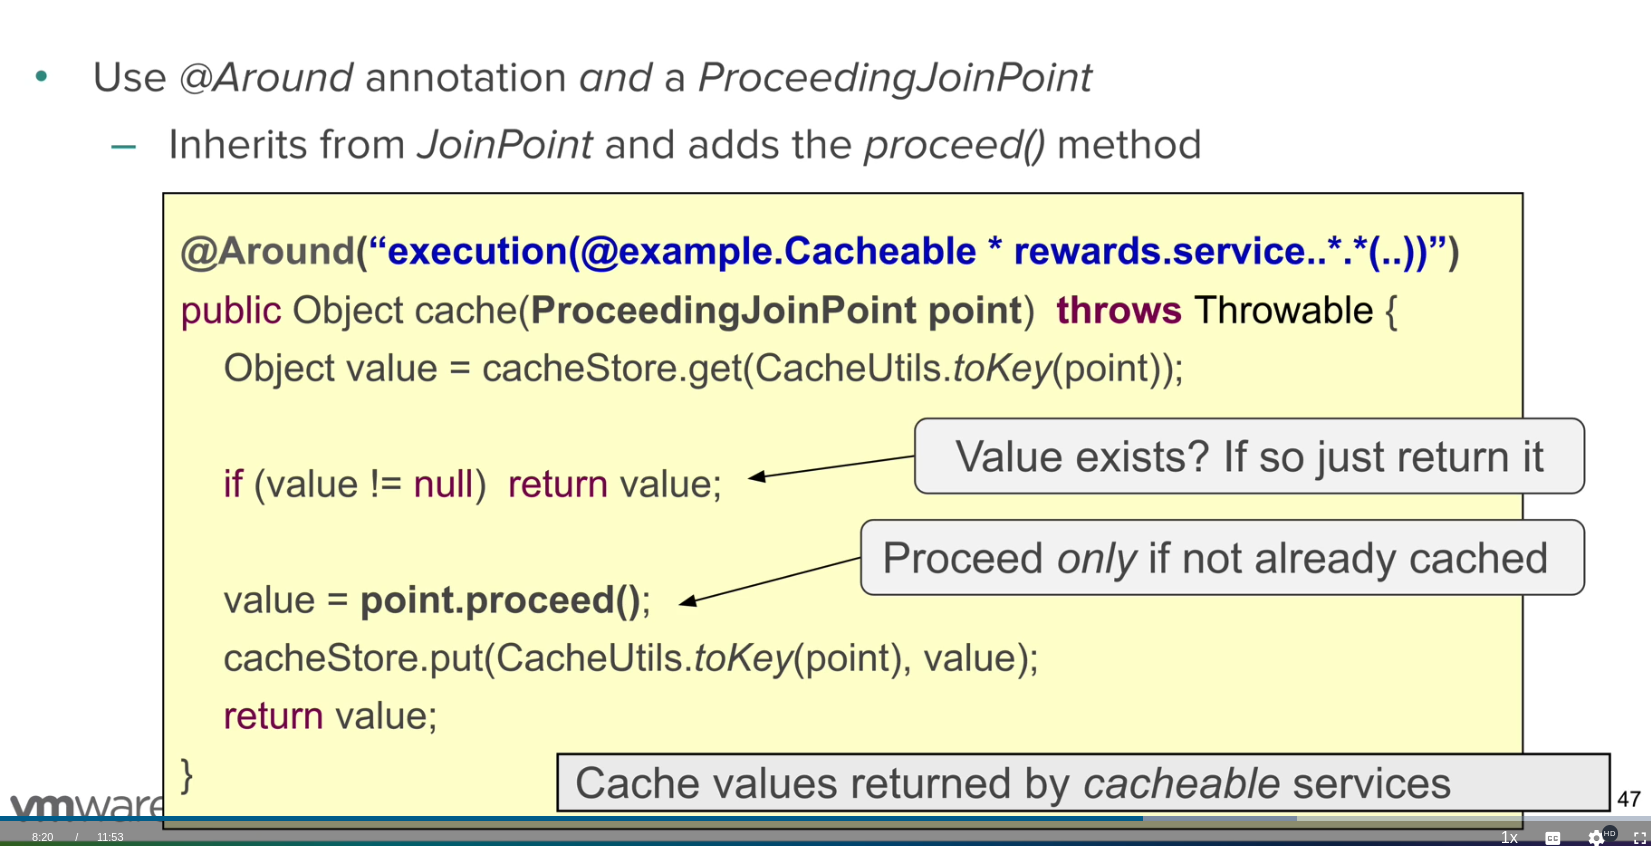
\includegraphics[width=1\linewidth]{around-advice}
        \caption{Around Advice}
        \label{fig:around-advice}
    \end{figure}

\end{itemize}

\subsubsection{Aspect}

The combination of point cut and advice. The @aspect annotation needs to be explicitly enabled by @EnableAspectJConfiguration set in the context (Config) class.

This will cause an extension of AbstractAutoProxyCreator to run, a BeanPostProcessor that wraps a bean with an AOP proxy. See \ref{fig:autoproxycreator}.

\begin{figure}
    \centering
    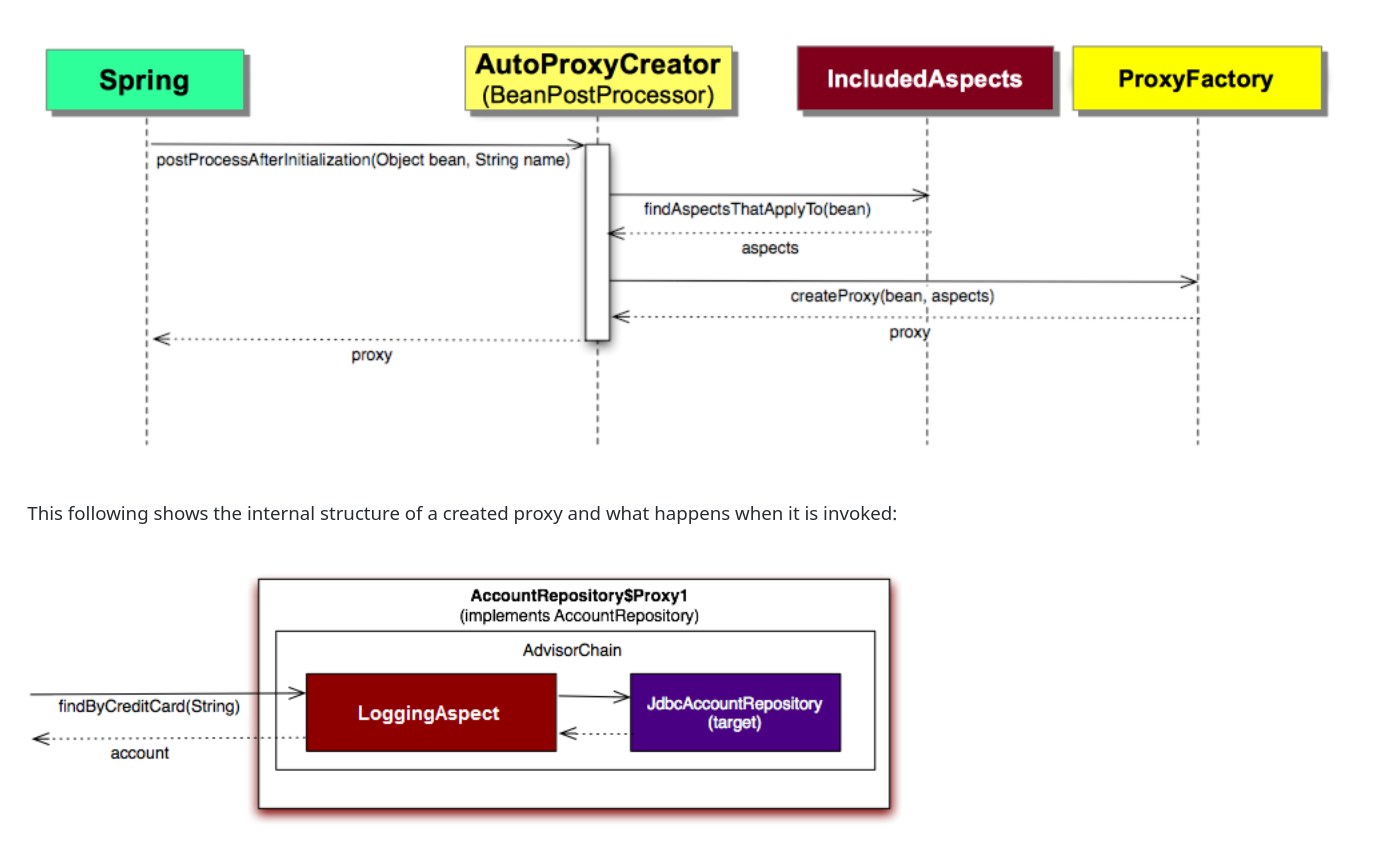
\includegraphics[width=1\linewidth]{autoproxycreator}
    \caption{Proxy Creation.}
    \label{fig:autoproxycreator}
\end{figure}

An aspect can get context information by injecting the JoinPoint into the advice. See fig. \ref{fig:AOP-join-point}.

\begin{figure}
    \centering
    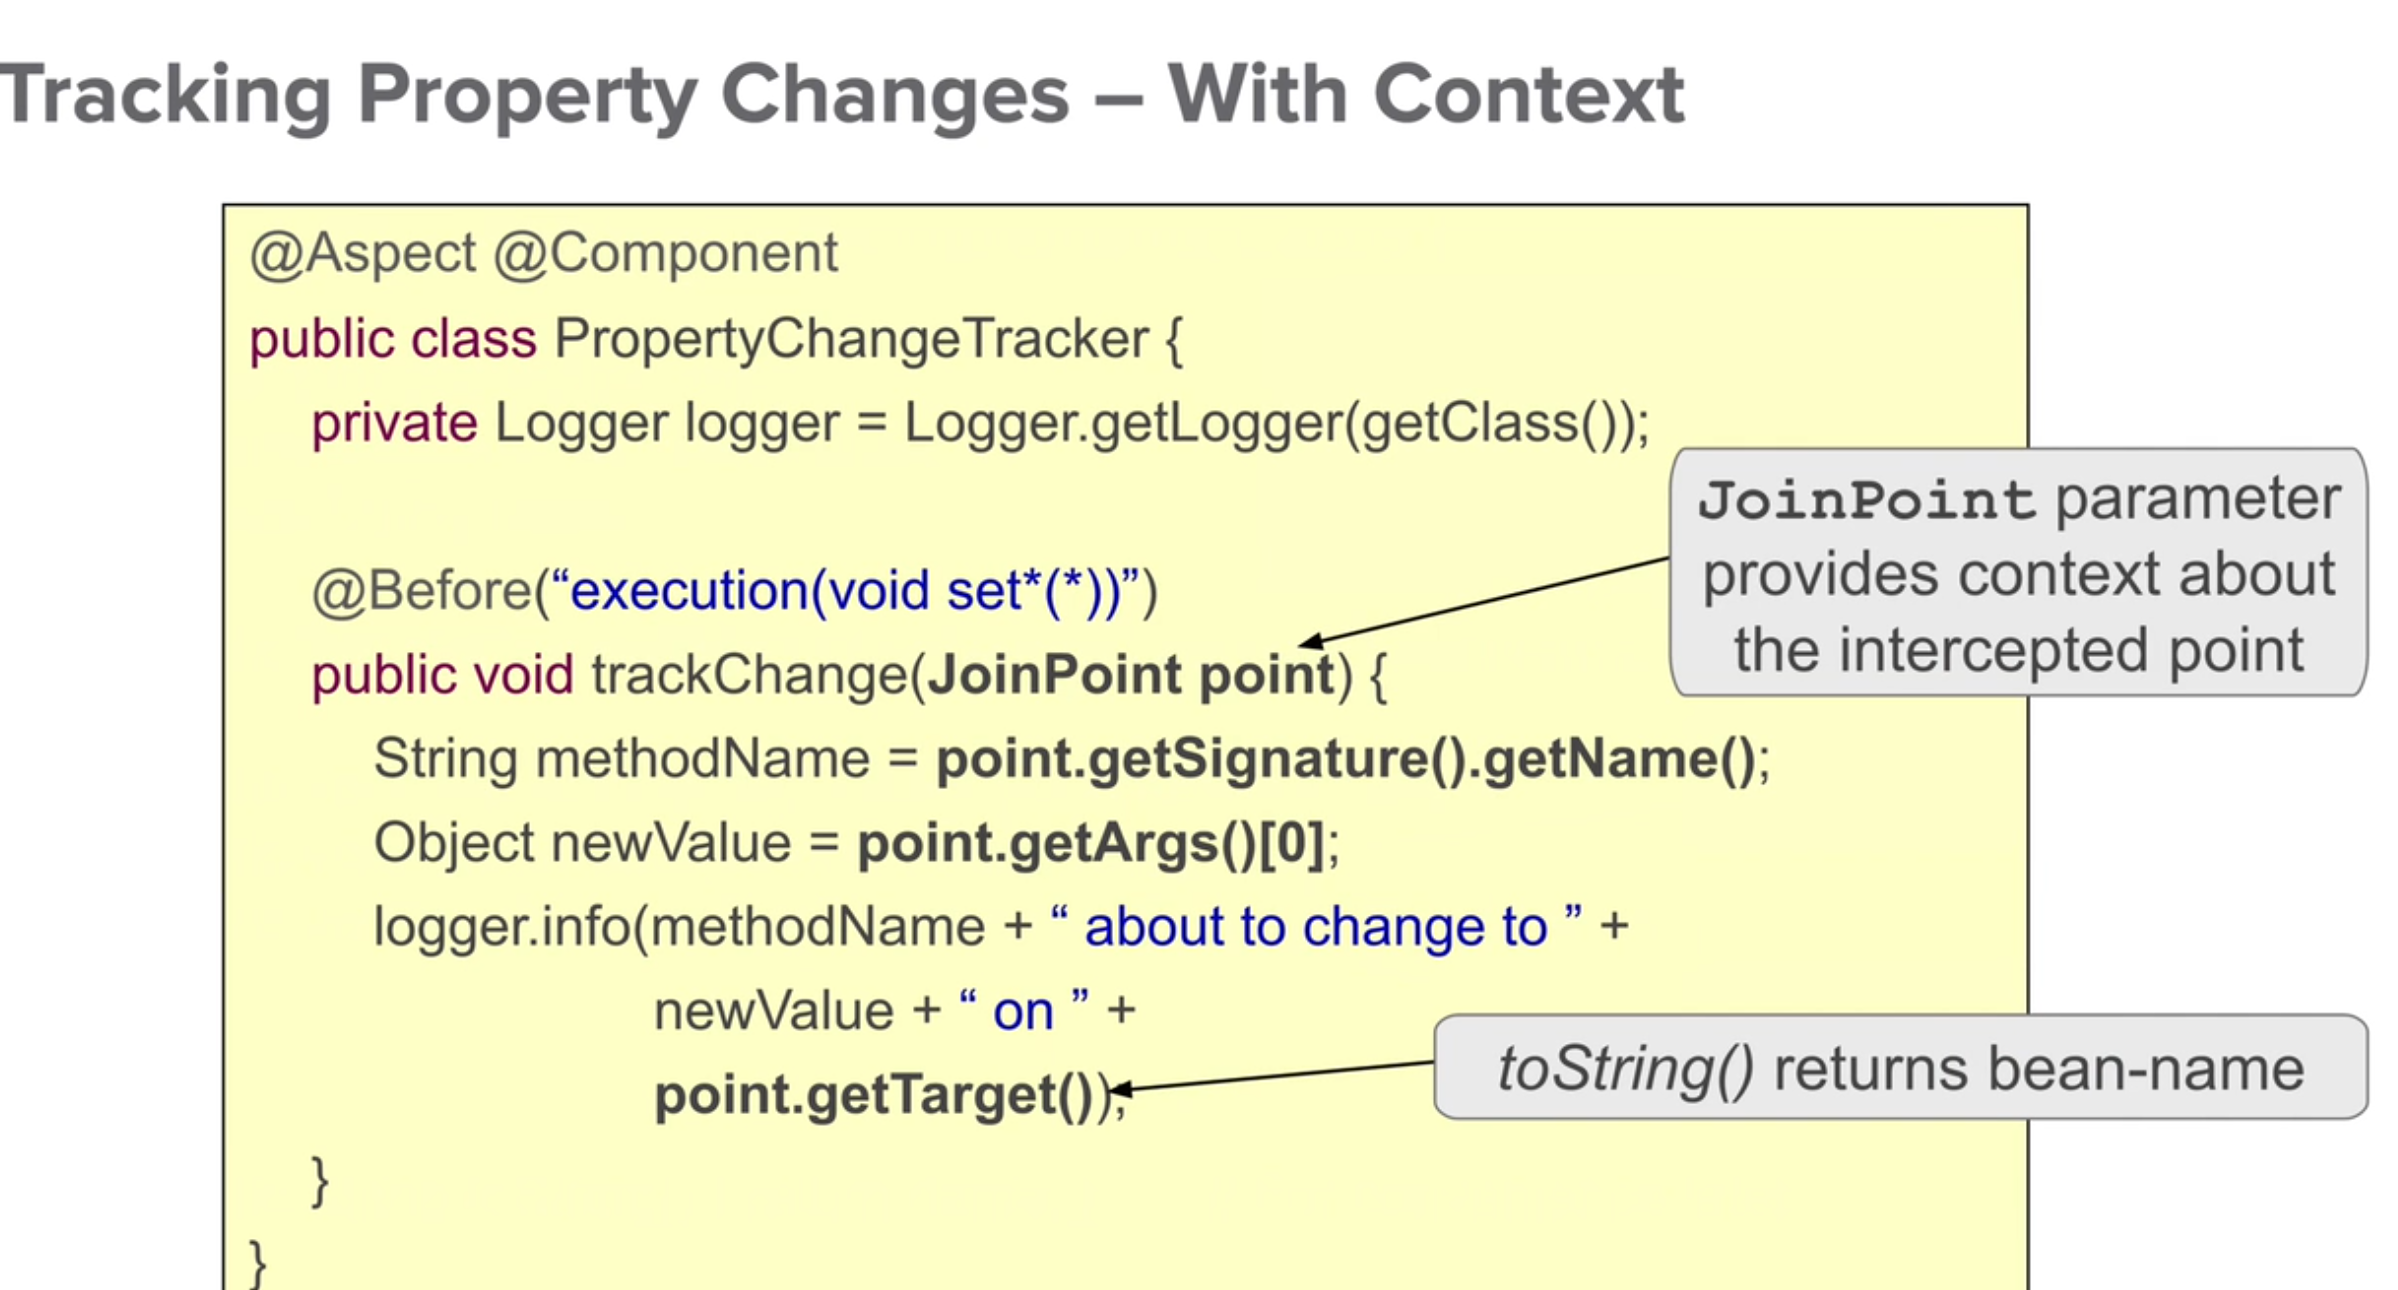
\includegraphics[width=1\linewidth]{AOP-join-point}
    \caption{Automatic JoinPoint injection}
    \label{fig:AOP-join-point}
\end{figure}

\begin{lstlisting}
    public abstract class AbstractAutoProxyCreator extends ProxyProcessorSupport
    implements SmartInstantiationAwareBeanPostProcessor, BeanFactoryAware {
        //...

        @Override
        public Object postProcessBeforeInstantiation(Class<?> beanClass, String beanName) {
            Object cacheKey = getCacheKey(beanClass, beanName);

            if (!StringUtils.hasLength(beanName) || !this.targetSourcedBeans.contains(beanName)) {
                if (this.advisedBeans.containsKey(cacheKey)) {
                    return null;
                }
                if (isInfrastructureClass(beanClass) || shouldSkip(beanClass, beanName)) {
                    this.advisedBeans.put(cacheKey, Boolean.FALSE);
                    return null;
                }
            }
        }

        @Override
        public Object postProcessAfterInitialization(@Nullable Object bean, String beanName) {
            if (bean != null) {
                Object cacheKey = getCacheKey(bean.getClass(), beanName);
                if (this.earlyProxyReferences.remove(cacheKey) != bean) {
                    return wrapIfNecessary(bean, beanName, cacheKey);
                }
            }
            return bean;
        }
    }
\end{lstlisting}

\subsubsection{More Terminology}

\textit{Introduction}
Declaring additional methods or fields on behalf of a type. Spring AOP lets you introduce new interfaces (and a corresponding implementation) to any advised object. For example, you could use an introduction to make a bean implement an IsModified interface, to simplify caching. (An introduction is known as an inter-type declaration in the AspectJ community.)

\textit{Target object}
An object being advised by one or more aspects. Also referred to as the "advised object". Since Spring AOP is implemented by using runtime proxies, this object is always a proxied object.

\textit{AOP proxy}
An object created by the AOP framework in order to implement the aspect contracts (advice method executions and so on). In the Spring Framework, an AOP proxy is a JDK dynamic proxy or a CGLIB proxy.

\textit{Weaving}
Linking aspects with other application types or objects to create an advised object. This can be done at compile time (using the AspectJ compiler, for example), load time, or at runtime. \textit{Spring AOP, like other pure Java AOP frameworks}, performs weaving at \textit{runtime}.

\subsection{AOP Proxies}

Spring AOP defaults to using standard\textit{ JDK dynamic proxies} for AOP proxies. This enables any interface (or set of interfaces) to be proxied.

Spring AOP can also use CGLIB proxies. This is necessary to proxy classes rather than interfaces. By default, CGLIB is used if a business object does not implement an interface.

If the target object to be proxied implements at least one interface, a JDK dynamic proxy is used, and all of the interfaces implemented by the target type are proxied. If the target object does not implement any interfaces, a CGLIB proxy is created which is a runtime-generated subclass of the target type.

\subsection{Implications of Using a Proxy}

Here, we create an object instance that calls a method on itself (using this).

\begin{lstlisting}
    public class SimplePojo implements Pojo {

        public void foo() {
            // this next method invocation is a direct call on the 'this' reference
            this.bar();
        }

        public void bar() {
            // some logic...
        }
    }

    public class Main {

        public static void main(String[] args) {
            Pojo pojo = new SimplePojo();
            // this is a direct method call on the 'pojo' reference
            pojo.foo();
        }
    }
\end{lstlisting}

When SimplePojo is proxied, the same call will not result in bar() being intercepted, since bar() is not called on the proxy, but the \lstinline[]|this| reference the object has to itself.

\begin{lstlisting}
    public class Main {

        public static void main(String[] args) {
            ProxyFactory factory = new ProxyFactory(new SimplePojo());
            factory.addInterface(Pojo.class);
            factory.addAdvice(new RetryAdvice());

            Pojo pojo = (Pojo) factory.getProxy();
            // this is a method call on the proxy!
            pojo.foo();
        }
    }
\end{lstlisting}

\subsection{Programmatic Creation of @AspectJ Proxies}

In addition to declaring aspects in your xml configuration by using either aop:config or aop:aspectj-autoproxy, it is also possible to programmatically create proxies that advise target objects.

You can use the org.springframework.aop.aspectj.annotation.AspectJProxyFactory class to create a proxy for a target object that is advised by one or more @AspectJ aspects.

\begin{lstlisting}
    // create a factory that can generate a proxy for the given target object
    AspectJProxyFactory factory = new AspectJProxyFactory(targetObject);

    // add an aspect, the class must be an @AspectJ aspect
    // you can call this as many times as you need with different aspects
    factory.addAspect(SecurityManager.class);

    // you can also add existing aspect instances, the type of the object supplied
    // must be an @AspectJ aspect
    factory.addAspect(usageTracker);

    // now get the proxy object...
    MyInterfaceType proxy = factory.getProxy();
\end{lstlisting}

\section{Transaction Management}

\subsection{Propagation Mode}









\begin{tabular}{|c|c|}
    \hline
    Enum Constant& Description \\
    \hline
    MANDATORY&  Support a current transaction, throw an exception if none exists.\\
    \hline
    NESTED&  Execute within a nested transaction if a current transaction exists, behave like REQUIRED otherwise.\\
    \hline
    NEVER &  Execute non-transactionally, throw an exception if a transaction exists.\\
    \hline
    NOT\_SUPPORTED& Execute non-transactionally, suspend the current transaction if one exists.\\
    \hline
    REQUIRED &  Support a current transaction, create a new one if none exists.\\
    \hline
    REQUIRES\_NEW &  Create a new transaction, and suspend the current transaction if one exists.\\
    \hline
    SUPPORTS&  Support a current transaction, execute non-transactionally if none exists.\\
    \hline
\end{tabular}

\subsection{Declarative}

The Spring Framework’s declarative transaction management is made possible with Spring aspect-oriented programming (AOP). Due to reliance on AOP, we can customize transactional behavior - for example, insert custom behavior in the case of transaction rollback, or add arbitrary advice, along with transactional advice.

The concept of rollback rules is important. They let you specify which exceptions (and throwables) should cause automatic rollback. You can specify this declaratively, in configuration, not in Java code. So, although you can still call \lstinline|setRollbackOnly()| on the TransactionStatus object to roll back the current transaction, most often you can specify a rule that MyApplicationException must always result in rollback.

The combination of AOP with transactional metadata yields an AOP proxy that uses a \lstinline|TransactionInterceptor| in conjunction with an appropriate \lstinline|TransactionManager| implementation to drive transactions around method invocations.

The following image shows a conceptual view of calling a method on a transactional proxy:

\begin{figure}[h]
    \centering
    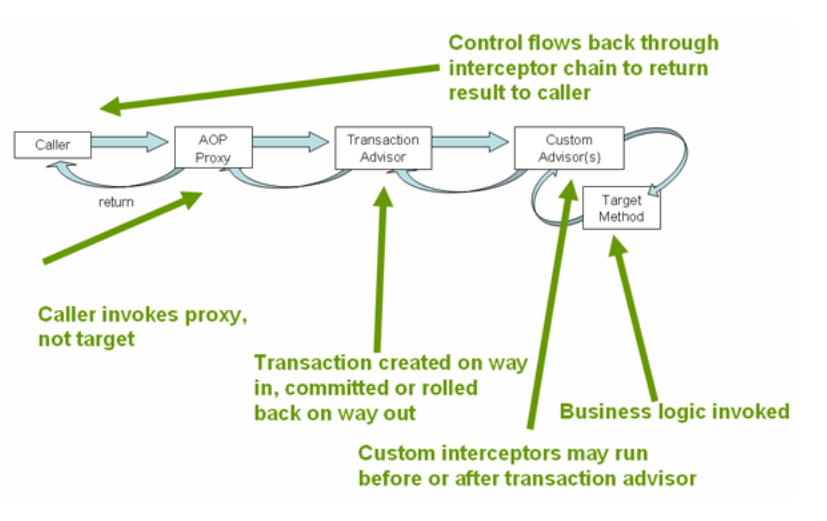
\includegraphics[width=1\linewidth]{transactions-aop}
    \caption{Spring Transaction Management Overview}
    \label{fig:transactions-aop}
\end{figure}

Since declarative transaction management is made possible using Spring AOP, which by default uses JDK Dynamic Proxies, only public methods called from outside the class are affected by the @Transactional annotation.

\subsection{Manual}

Instead of using the @Transactional annotation, transactions can be managed programmatically using TransactionTemplate.

To be used, it needs to be initialized it with a PlatformTransactionManager.

Example:

\begin{lstlisting}
    class ManualTransactionIntegrationTest {

        @Autowired
        private PlatformTransactionManager transactionManager;

        private TransactionTemplate transactionTemplate;

        @BeforeEach
        void setUp() {
            transactionTemplate = new TransactionTemplate(transactionManager);
        }

        // omitted
    }
\end{lstlisting}

When using Spring Boot, an appropriate bean of type PlatformTransactionManager will be automatically registered, so we just need to inject it. Otherwise, we have to manually register a PlatformTransactionManager bean.

The correct order of operations when using TransactionTemplate in programmatic transaction management is:

\begin{itemize}
    \item begin transaction
    \item execute callback (which contains the transactional code)
    \item commit transaction if the callback executes successfully
    \item rollback transaction if an exception occurs during callback execution
\end{itemize}

\section{Data Access with JDBC}

The following table shows which actions Spring takes care of and which actions are your responsibility.

\begin{table}[h!]
\begin{tabular}{|r|c|c|}
    \hline
    Action&  Spring&  You\\
    \hline
    Define connection parameters&  &  x\\
    \hline
    Open the connection.&  x&  \\
    \hline
    Specify the SQL statement.&  &  x\\
    \hline
    Declare parameters and provide parameter values&  &  x\\
    \hline
    Prepare and run the statement.&  x&  \\
    \hline
    Set up the loop to iterate through the results (if any).&  x&  \\
    \hline
    Do the work for each iteration.&  &  x\\
    \hline
    Process any exception.&  x&  \\
    \hline
    Handle transactions.&  x&  \\
    \hline
    Close the connection, the statement, and the resultset.&  x&  \\
    \hline
\end{tabular}
\end{table}

\subsection{Package Hierarchy}

The Spring Framework’s JDBC abstraction framework consists of four different packages:

\begin{itemize}
    \item core: The org.springframework.jdbc.core package contains the JdbcTemplate class and its various callback interfaces, plus a variety of related classes. A subpackage named org.springframework.jdbc.core.simple contains the SimpleJdbcInsert and SimpleJdbcCall classes. Another subpackage named org.springframework.jdbc.core.namedparam contains the NamedParameterJdbcTemplate class and the related support classes. See Using the JDBC Core Classes to Control Basic JDBC Processing and Error Handling, JDBC Batch Operations, and Simplifying JDBC Operations with the SimpleJdbc Classes.

    \item datasource: The org.springframework.jdbc.datasource package contains a utility class for easy DataSource access and various simple DataSource implementations that you can use for testing and running unmodified JDBC code outside of a Jakarta EE container. A subpackage named org.springframework.jdbc.datasource.embedded provides support for creating embedded databases by using Java database engines, such as HSQL, H2, and Derby. See Controlling Database Connections and Embedded Database Support.

    \item object: The org.springframework.jdbc.object package contains classes that represent RDBMS queries, updates, and stored procedures as thread-safe, reusable objects. See Modeling JDBC Operations as Java Objects. This style results in a more object-oriented approach, although objects returned by queries are naturally disconnected from the database. This higher-level of JDBC abstraction depends on the lower-level abstraction in the org.springframework.jdbc.core package.

    \item support: The org.springframework.jdbc.support package provides SQLException translation functionality and some utility classes. Exceptions thrown during JDBC processing are translated to exceptions defined in the org.springframework.dao package. This means that code using the Spring JDBC abstraction layer does not need to implement JDBC or RDBMS-specific error handling. All translated exceptions are unchecked, which gives you the option of catching the exceptions from which you can recover while letting other exceptions be propagated to the caller. See Using SQLExceptionTranslator.
\end{itemize}

\subsection{Using JdbcTemplate}

JdbcTemplate acquires a database connection only during a method call, which requires data access, and releases it as soon as the rows are fetched.

\subsubsection{Queries}

Examples:

\begin{lstlisting}

    Actor actor = jdbcTemplate.queryForObject(
    "select first_name, last_name from t_actor where id = ?",
    (resultSet, rowNum) -> {
        Actor newActor = new Actor();
        newActor.setFirstName(
            resultSet.getString("first_name"));
        newActor.setLastName(
            resultSet.getString("last_name"));
        return newActor;
    },
    1212L);

    List<Actor> actors = this.jdbcTemplate.query(
    "select first_name, last_name from t_actor",
    (resultSet, rowNum) -> {
        Actor actor = new Actor();
        actor.setFirstName(
            resultSet.getString("first_name"));
        actor.setLastName(
            resultSet.getString("last_name"));
        return actor;
    });

    // If the last two snippets of code actually existed in the same application, it would make sense to remove the duplication present in the two RowMapper lambda expressions and extract them out into a single field that could then be referenced by DAO methods as needed. For example, it may be better to write the preceding code snippet as follows:

    private final RowMapper<Actor> actorRowMapper = (resultSet, rowNum) -> {
        Actor actor = new Actor();
        actor.setFirstName(
            resultSet.getString("first_name"));
        actor.setLastName(
            resultSet.getString("last_name"));
        return actor;
    };

    public List<Actor> findAllActors() {
        return this.jdbcTemplate.query("select first_name, last_name from t_actor", actorRowMapper);
    }
\end{lstlisting}

\subsubsection{Updating (INSERT, UPDATE, and DELETE) with JdbcTemplate}

You can use the update(..) method to perform insert, update, and delete operations. Parameter values are usually provided as variable arguments or, alternatively, as an object array.

\begin{lstlisting}
     //The following example inserts a new entry:
    this.jdbcTemplate.update(
    "insert into t_actor (first_name, last_name) values (?, ?)",
    "Leonor", "Watling");

    //The following example updates an existing entry:
    this.jdbcTemplate.update(
    "update t_actor set last_name = ? where id = ?",
    "Banjo", 5276L);

    //The following example deletes an entry:
    this.jdbcTemplate.update(
    "delete from t_actor where id = ?",
    Long.valueOf(actorId));
\end{lstlisting}

\subsubsection{Other JdbcTemplate Operations}

You can use the execute(..) method to run any arbitrary SQL. Consequently, the method is often used for DDL statements. It is heavily overloaded with variants that take callback interfaces, binding variable arrays, and so on.

\begin{lstlisting}
    //The following example creates a table:
    this.jdbcTemplate.execute("create table mytable (id integer, name varchar(100))");

    //The following example invokes a stored procedure:
    this.jdbcTemplate.update(
    "call SUPPORT.REFRESH_ACTORS_SUMMARY(?)",
    Long.valueOf(unionId));
\end{lstlisting}

\subsubsection{Callback interfaces }

JdbcTemplate callback interfaces (functional interfaces; implementors must implement the abstract method):

\begin{tabular}{|c|c|c|}
    \hline
    RowCallbackHandler&  processRow(ResultSet rs)& process each row
    \\
    \hline
    ResultSetExtractor \textless T \textgreater& extractData(ResultSet rs)
    & process entire ResultSet\\
    \hline
    RowMapper \textless T \textgreater& mapRow(ResultSet rs, int rowNum)
    &  map each row \\
    \hline
\end{tabular}


\section{Data Access with JPA}
\subsection{Repository Query Language}

Example (see \url{  https://docs.spring.io/spring-data/commons/reference/repositories/query-methods-details.html}):


\begin{lstlisting}
   interface PersonRepository extends Repository<Person, Long> {

       List<Person> findByEmailAddressAndLastname(EmailAddress emailAddress, String lastname);

       // Enables the distinct flag for the query
       List<Person> findDistinctPeopleByLastnameOrFirstname(String lastname, String firstname);
       List<Person> findPeopleDistinctByLastnameOrFirstname(String lastname, String firstname);

       // Enabling ignoring case for an individual property
       List<Person> findByLastnameIgnoreCase(String lastname);
       // Enabling ignoring case for all suitable properties
       List<Person> findByLastnameAndFirstnameAllIgnoreCase(String lastname, String firstname);

       // Enabling static ORDER BY for a query
       List<Person> findByLastnameOrderByFirstnameAsc(String lastname);
       List<Person> findByLastnameOrderByFirstnameDesc(String lastname);
   }
\end{lstlisting}

\subsection{Reserved Method Names}

    Reserved methods like CrudRepository.findById (or just findById) are targeting the identifier property regardless of the actual property name used in the declared method.
    Example:

\begin{lstlisting}
    class User {
        //The identifier property (primary key).
        @Id Long pk;

        // A property named id, but not the identifier.
        Long id;
    }

    interface UserRepository extends Repository<User, Long> {

        // Targets the pk property (the one marked with @Id which is considered to be the identifier) as it refers to a CrudRepository base repository method.
        Optional<User> findById(Long id);

        // Targets the pk property by name as it is a derived query.
        Optional<User> findByPk(Long pk);

        // Targets the id property by using the descriptive token between find and by to avoid collisions with reserved methods.
        Optional<User> findUserById(Long id);
    }

\end{lstlisting}

\subsection{Using explicitly defined queries}

To explicitly define queries, the annotation @Query can be used.

The queries themselves are tied to the Java method that executes them, you can actually bind them directly by using the Spring Data JPA @Query annotation rather than annotating them to the domain class. This frees the domain class from persistence specific information and co-locates the query to the repository interface.

Queries annotated to the query method take precedence over queries defined using @NamedQuery or named queries declared in orm.xml.

Example:

\begin{lstlisting}
    public interface UserRepository extends JpaRepository<User, Long> {

    @Query("select u from User u where u.emailAddress = ?1")
    User findByEmailAddress(String emailAddress);
}

\end{lstlisting}


\subsection{Paging, Iterating Large Results, Sorting and Limiting}

    Spring recognizes certain specific types like Pageable, Sort and Limit, to apply pagination, sorting and limiting to your queries dynamically.
    Example:

\begin{lstlisting}
    Page<User> findByLastname(String lastname, Pageable pageable);

    Slice<User> findByLastname(String lastname, Pageable pageable);

    List<User> findByLastname(String lastname, Sort sort);

    List<User> findByLastname(String lastname, Sort sort, Limit limit);

    List<User> findByLastname(String lastname, Pageable pageable);
\end{lstlisting}

\subsection{Repository Query Keywords}

\begin{lstlisting}
    // General query method returning typically the repository type, a Collection or Streamable subtype or a result wrapper such as Page, GeoResults or any other store-specific result wrapper. Can be used as findBy..., findMyDomainTypeBy... or in combination with additional keywords.
    find...By, read...By, get...By, query...By, search...By, stream...By

    // Exists projection, returning typically a boolean result.
    exists...By

    // Count projection returning a numeric result.
    count...By

    //  Delete query method returning either no result (void) or the delete count.
    delete...By, remove...By

    //  Limit the query results to the first <number> of results. This keyword can occur in any place of the subject between find (and the other keywords) and by.
    ...First<number>..., ...Top<number>...

    //  Use a distinct query to return only unique results. Consult the store-specific documentation whether that feature is supported. This keyword can occur in any place of the subject between find (and the other keywords) and by.
    ...Distinct...
\end{lstlisting}

\subsection{Supported query method predicate keywords and modifiers}

\begin{table}[ht]
\begin{tabular}{ | r | r |}
    \hline
    Logical keyword &	Keyword expressions \\
    \hline
    AND & And \\
    OR &  Or \\
    AFTER & After, IsAfter \\
    BEFORE & Before, IsBefore\\
    CONTAINING&Containing, IsContaining, Contains\\
    BETWEEN&Between, IsBetween\\
    ENDING\_WITH&EndingWith, IsEndingWith, EndsWith\\
    EXISTS&Exists\\
    FALSE&False, IsFalse\\
    GREATER\_THAN&GreaterThan, IsGreaterThan\\
    GREATER\_THAN\_EQUALS&GreaterThanEqual, IsGreaterThanEqual\\
    IN&In, IsIn\\
    IS&Is, Equals, (or no keyword)\\
    IS\_EMPTY&IsEmpty, Empty\\
    IS\_NOT\_EMPTY&IsNotEmpty, NotEmpty\\
    IS\_NOT\_NULL&NotNull, IsNotNull\\
    IS\_NULL&Null, IsNull\\
    LESS\_THAN&LessThan, IsLessThan\\
    LESS\_THAN\_EQUAL&LessThanEqual, IsLessThanEqual\\
    LIKE&Like, IsLike\\
    NEAR&Near, IsNear\\
    NOT&Not, IsNotNOT\_INNotIn, IsNotIn\\
    NOT\_LIKE&NotLike, IsNotLike\\
    REGEX&Regex, MatchesRegex, Matches\\
    STARTING\_WITH&StartingWith, IsStartingWith, StartsWith\\
    TRUE&True, IsTrue\\
    WITHIN&Within, IsWithin\\
    \hline
\end{tabular}
\end{table}

    In addition to filter predicates, the following list of modifiers is supported:
    \begin{itemize}
        \item IgnoreCase, IgnoringCase
        \item AllIgnoreCase, AllIgnoringCase
        \item OrderBy... (e. g. OrderByFirstnameAscLastnameDesc).
    \end{itemize}




\section{Spring Security}
\subsection{Overview}

Spring Security provides a Filter implementation named \lstinline|DelegatingFilterProxy| that allows bridging between the Servlet container’s lifecycle and Spring’s ApplicationContext.


Architecture Overview (see \ref{fig:spring-security}):

\begin{figure}[h]
    \centering
    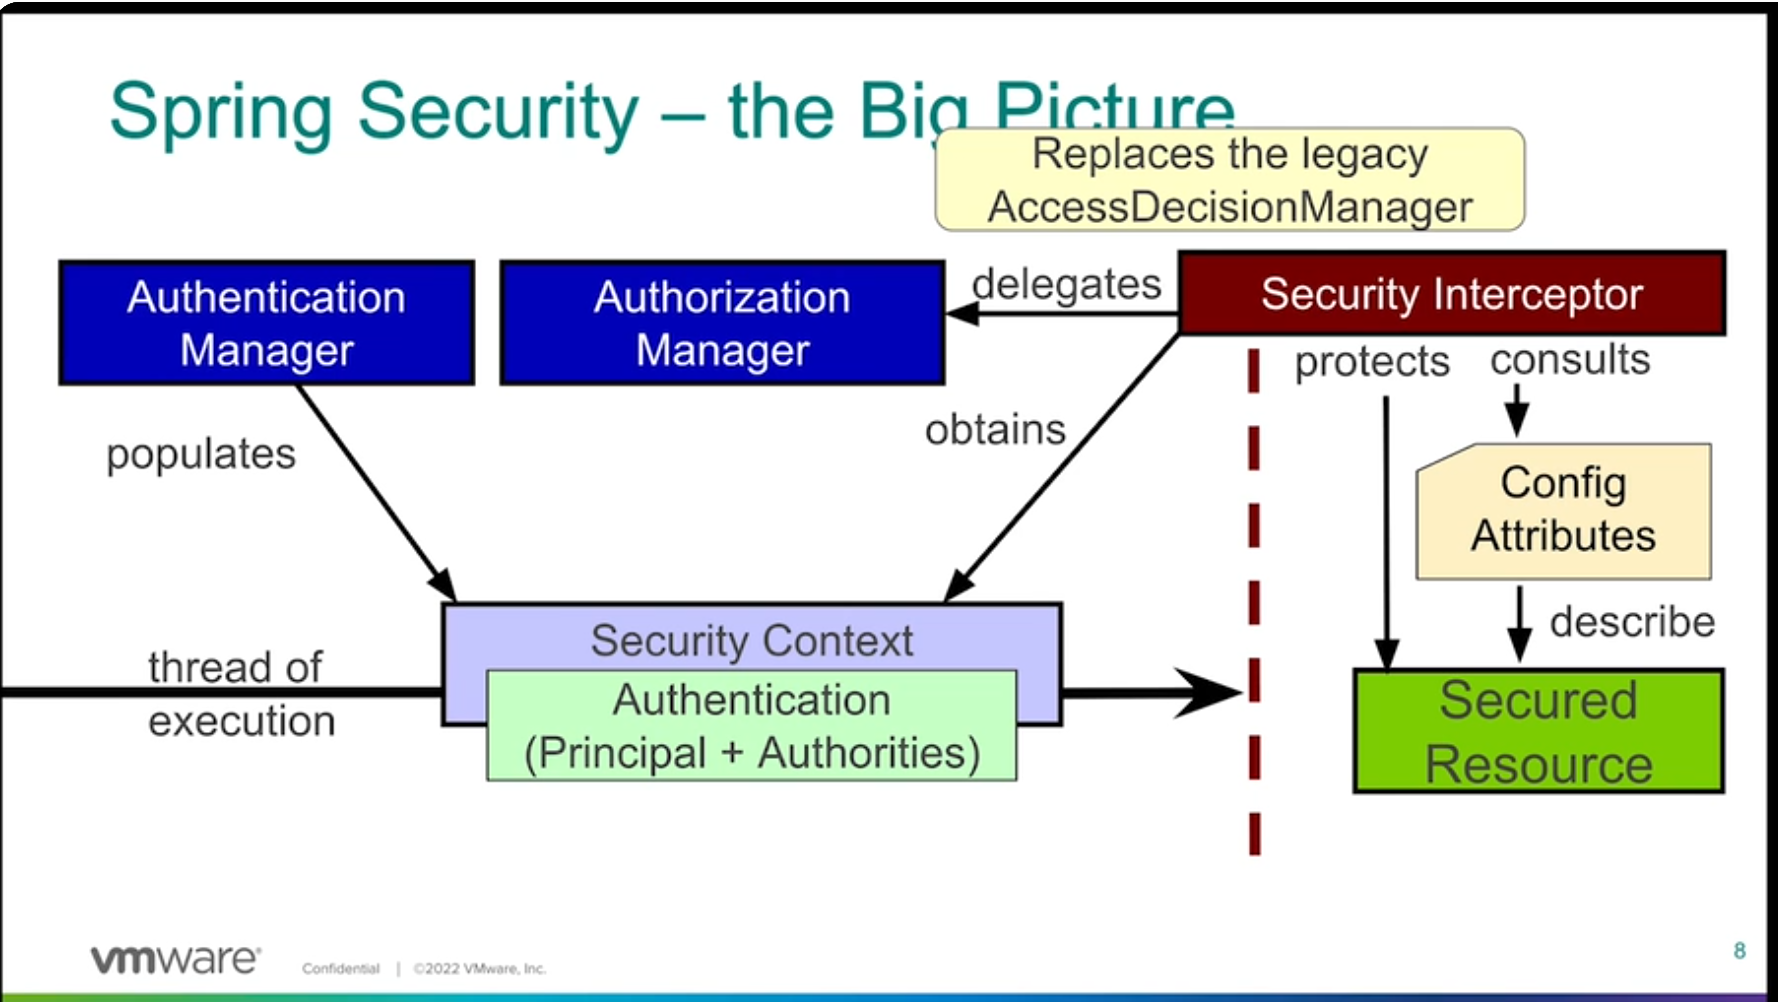
\includegraphics[width=1\linewidth]{spring-security}
    \caption{Spring Security Architecture Overview}
    \label{fig:spring-security}
\end{figure}

\subsection{Filter Chain}

Overview (see \ref{fig:filter-chain}):

\begin{figure}[h]
    \centering
    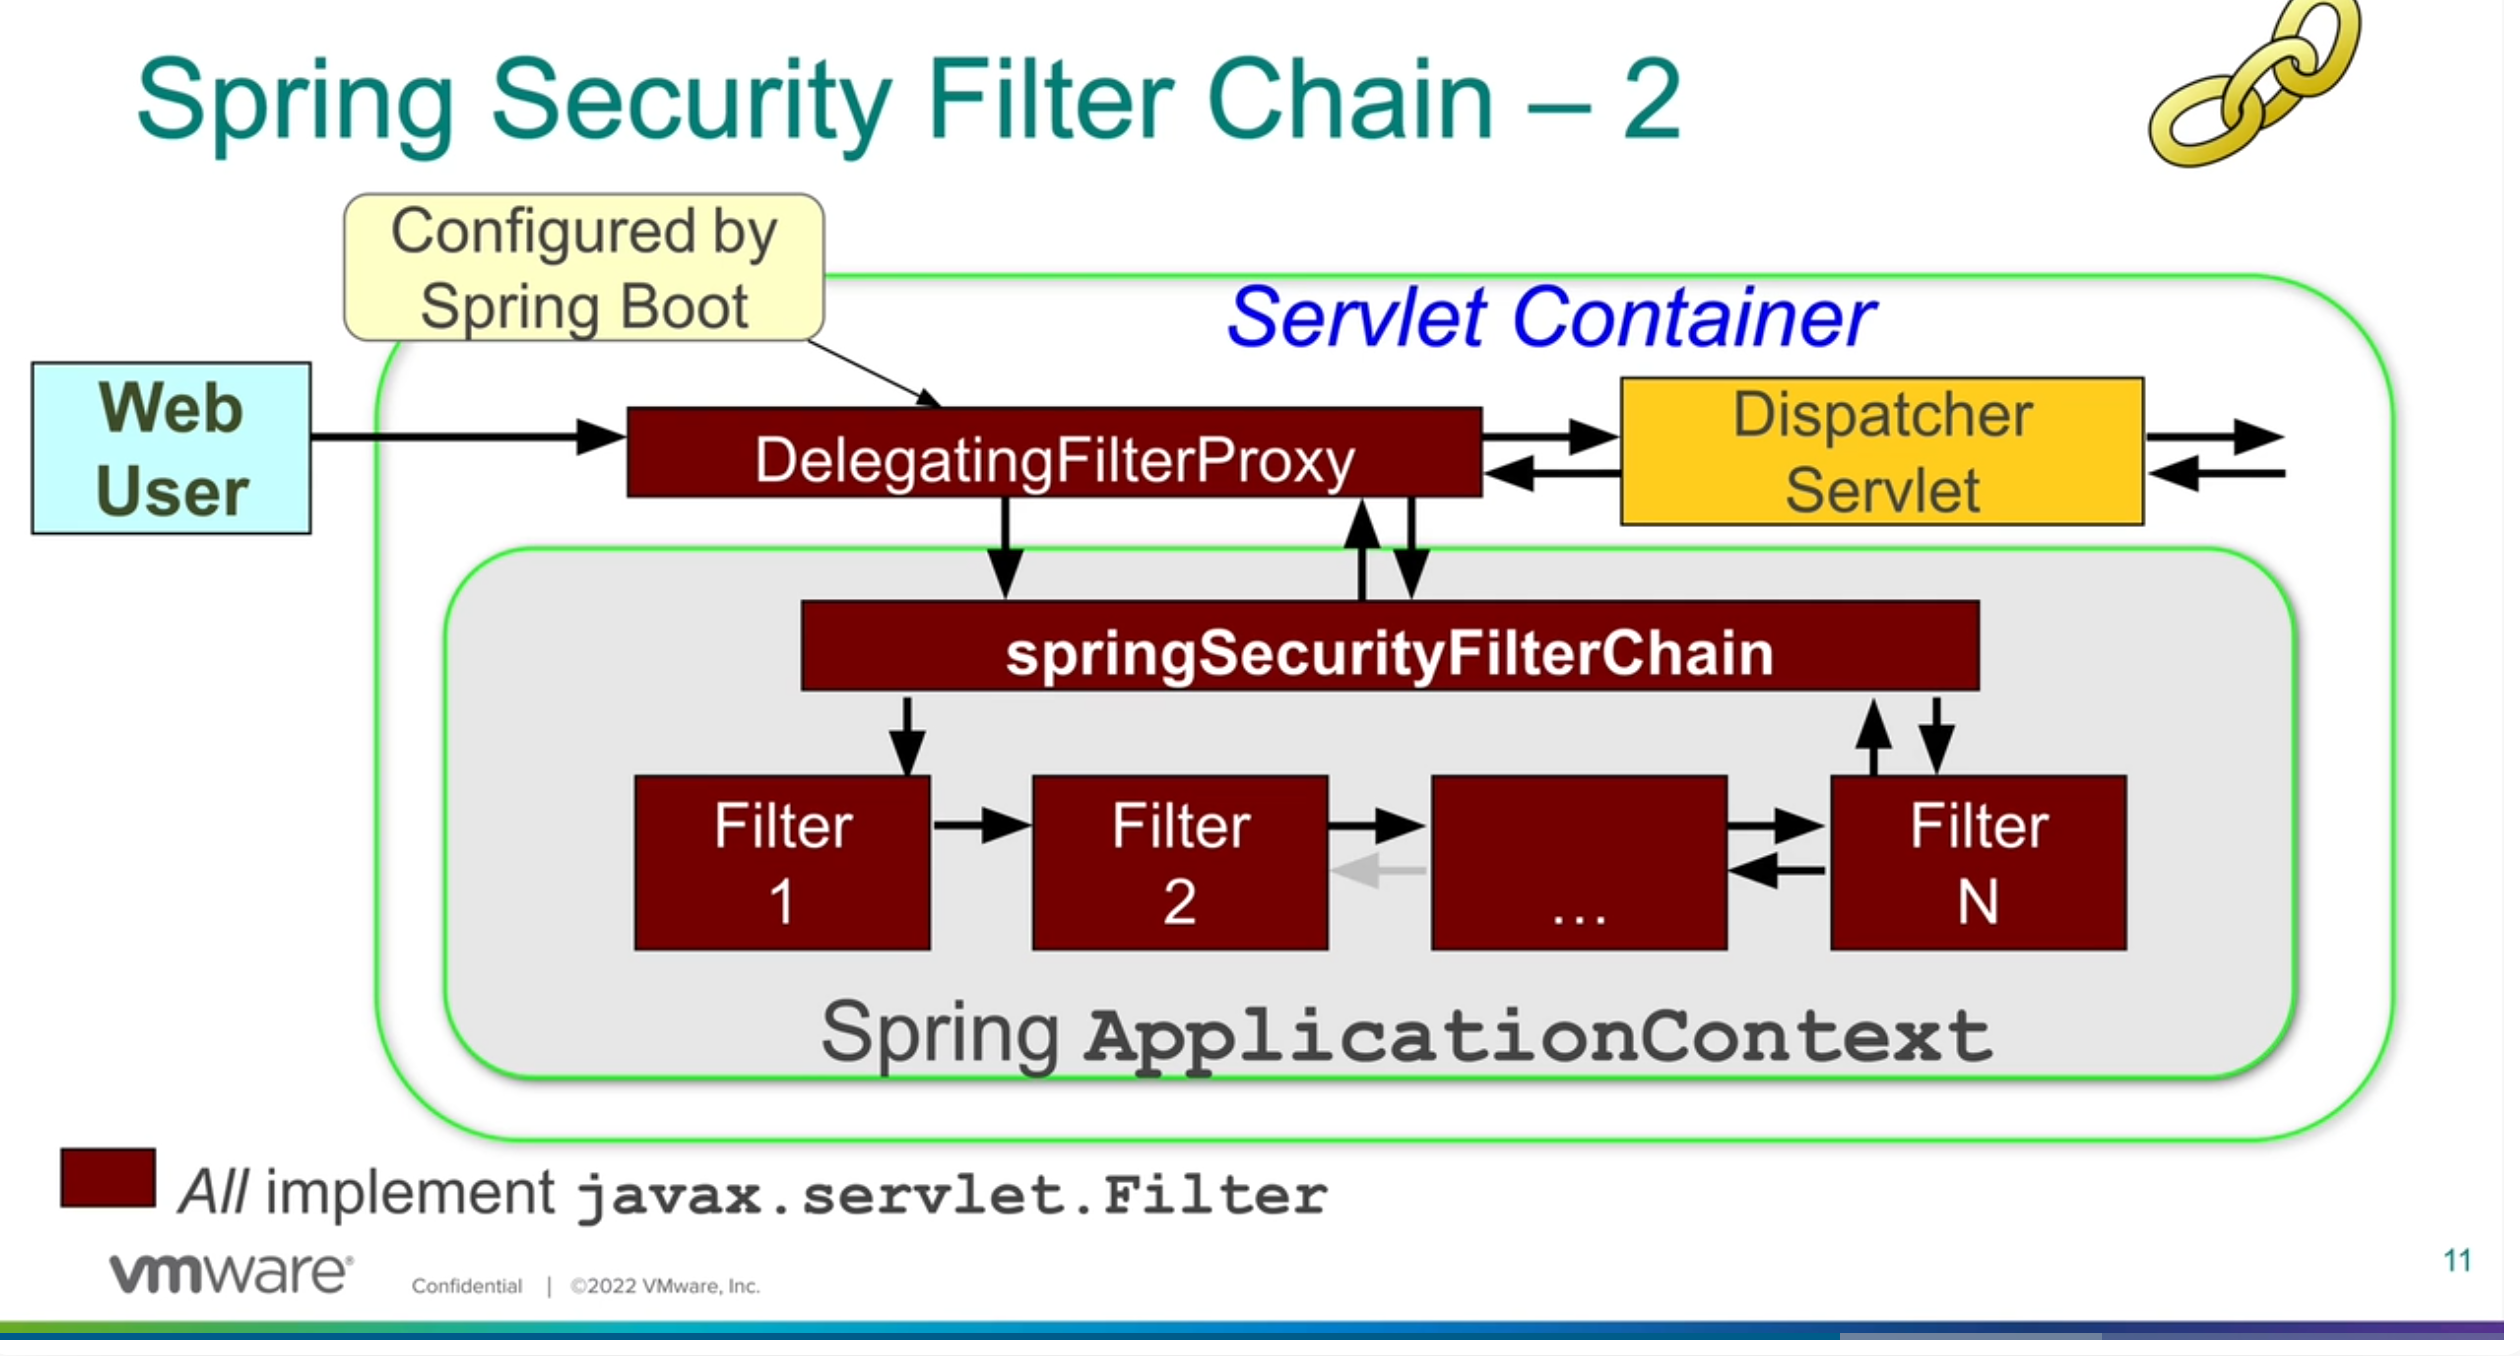
\includegraphics[width=1\linewidth]{filter-chain}
    \caption{Spring Security Filter Chain}
    \label{fig:filter-chain}
\end{figure}

Example (see \ref{fig:filter-chain-example}):

\begin{figure} [h]
    \centering
    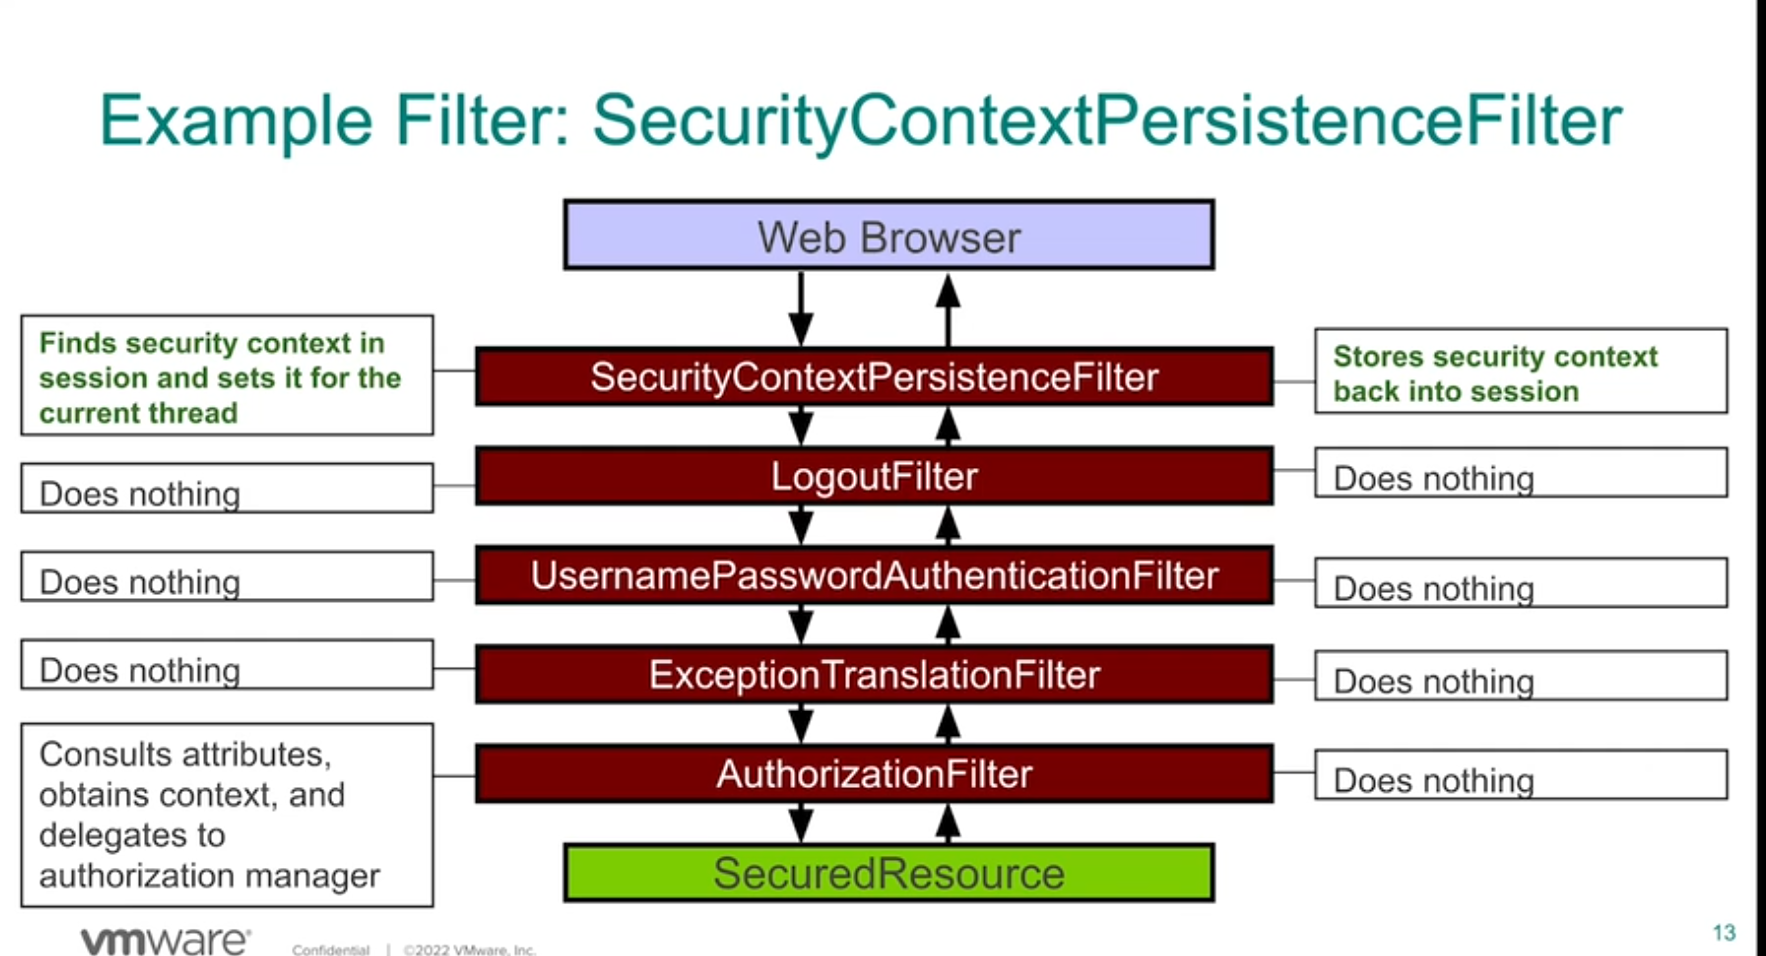
\includegraphics[width=1\linewidth]{filter-chain-example}
    \caption{Example Filter Chain}
    \label{fig:filter-chain-example}
\end{figure}

\subsection{Authentication}

Spring Security offers the following authentication mechanisms: Username and Password, OAuth 2.0, SAML 2.0, CAS, Remember Me, JAAS Authentication, OpenID, Pre-Authentication Scenarios and X509 Authentication.

Overview (see \ref{fig:authentication}):

\begin{figure}[h]
    \centering
    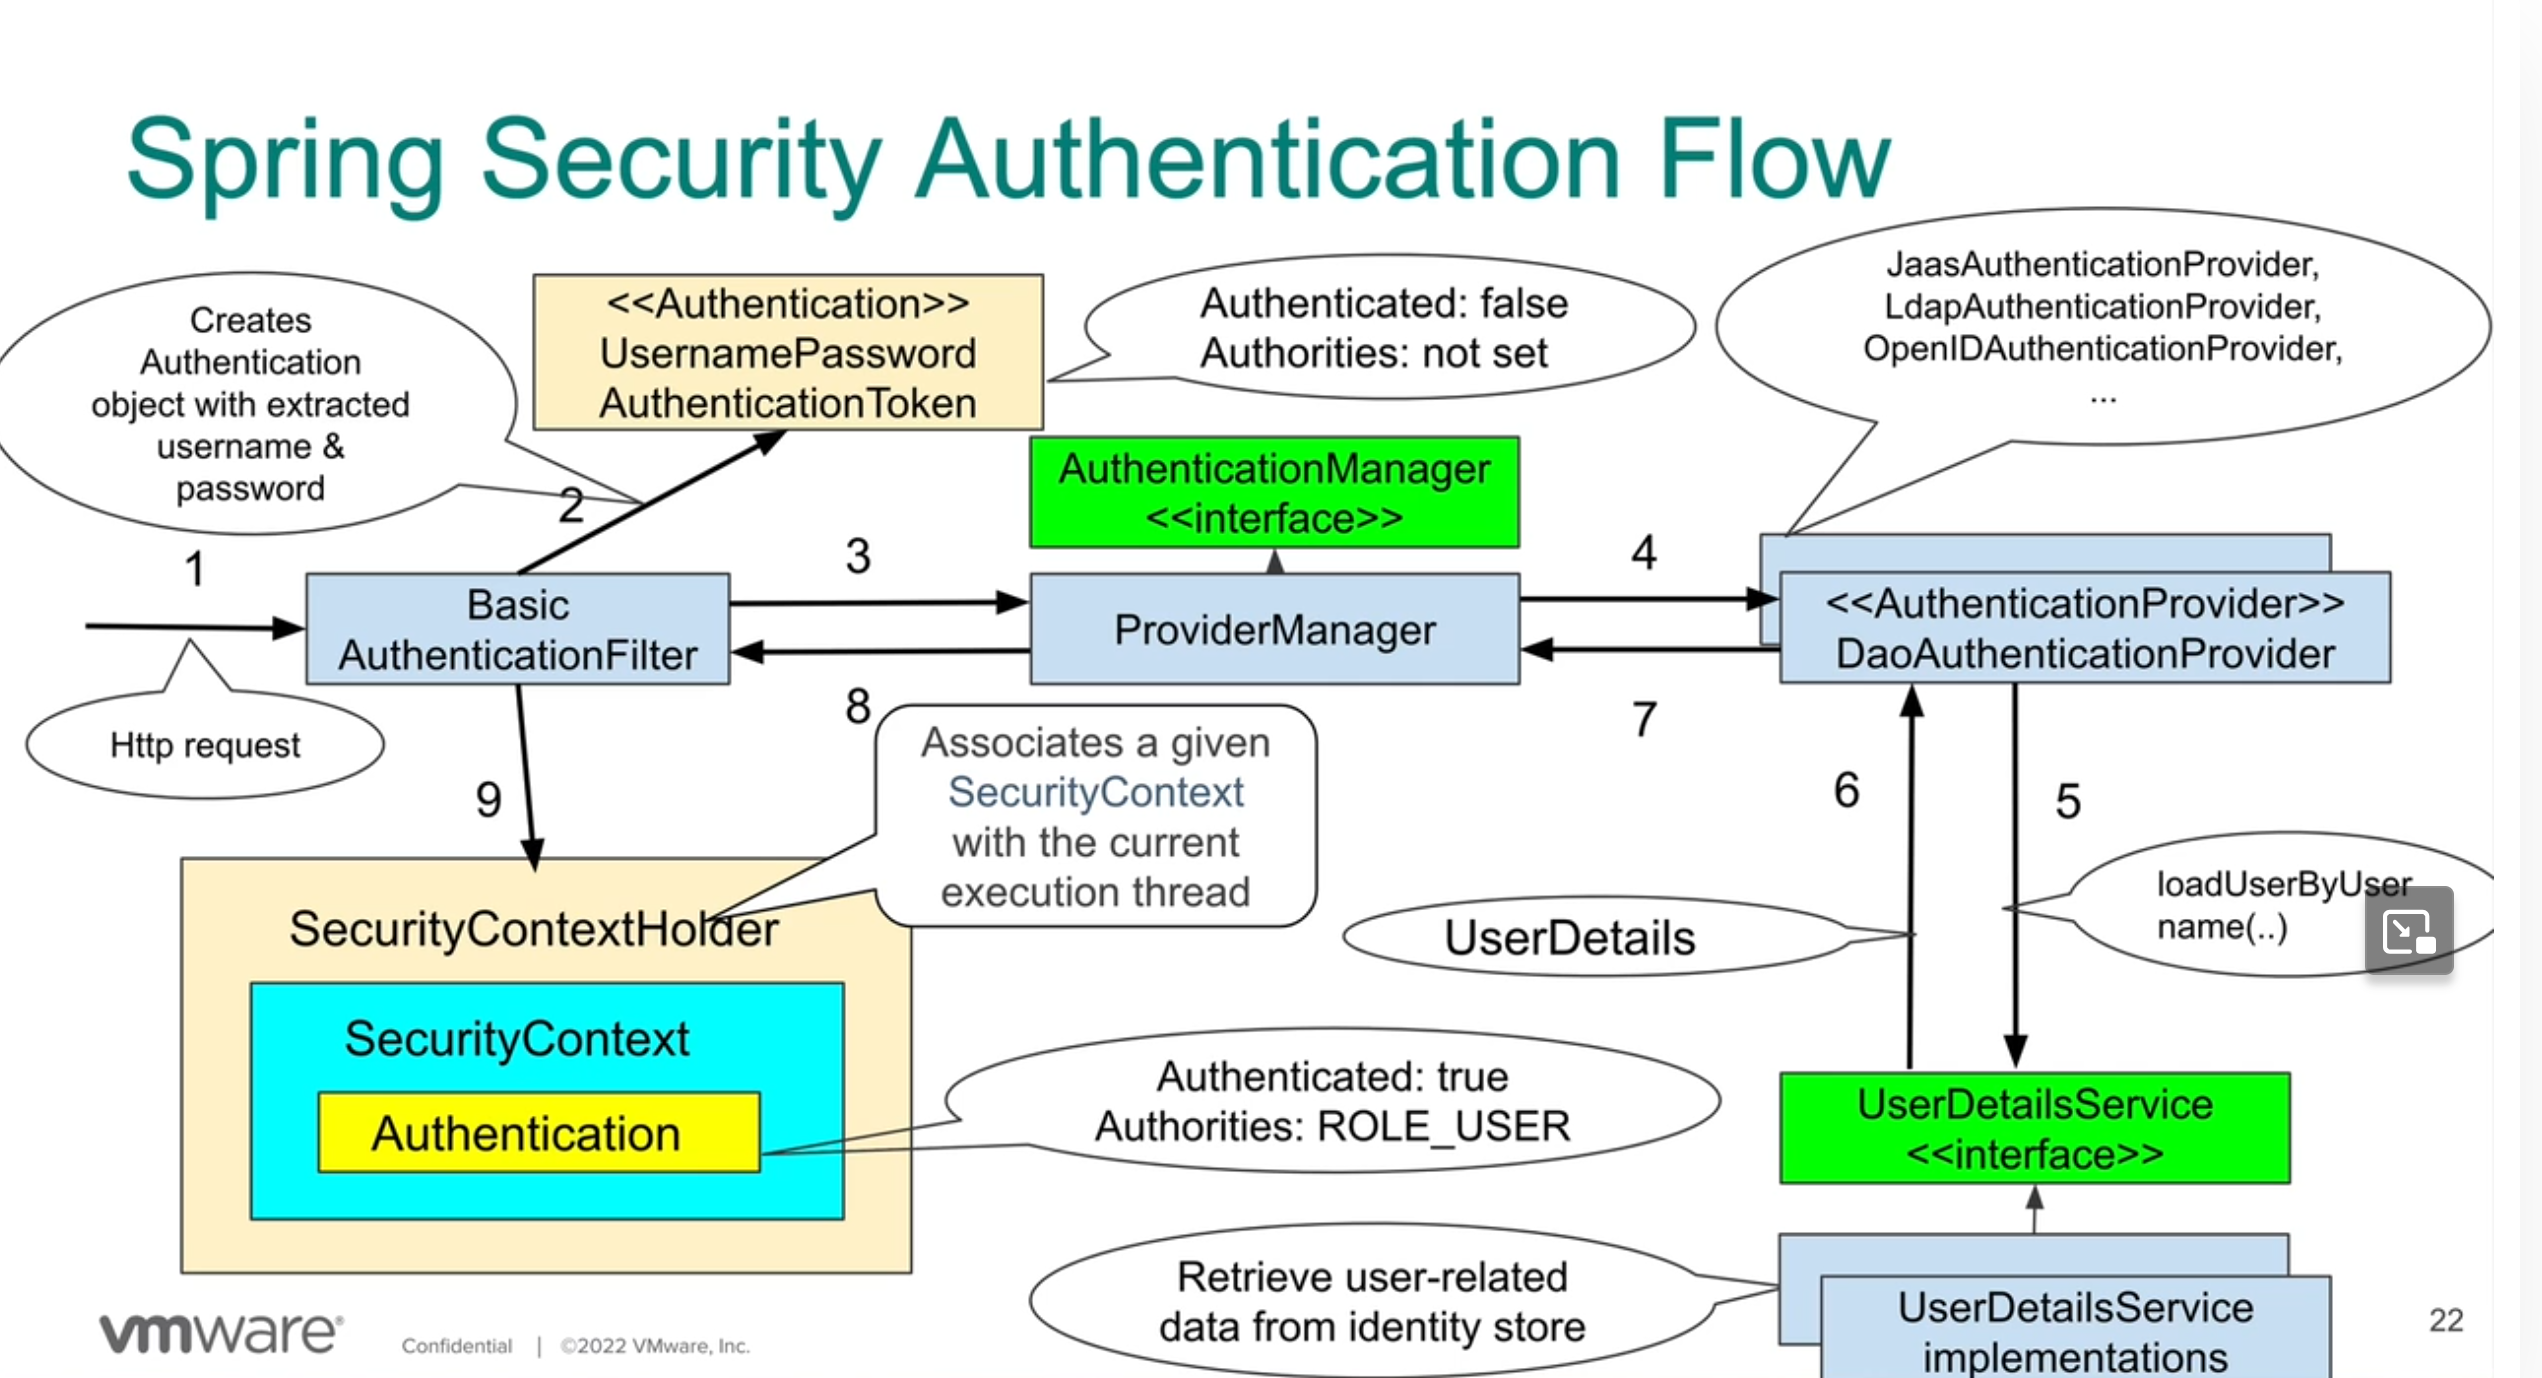
\includegraphics[width=1\linewidth]{authentication}
    \caption{Spring Security Filter Chain}
    \label{fig:authentication}
\end{figure}
\subsection{Authorization}

All Authentication implementations store a list of GrantedAuthority objects. These represent the authorities that have been granted to the principal. The GrantedAuthority objects are inserted into the Authentication object by the AuthenticationManager and are later read by AuthorizationManager instances when making authorization decisions.

The GrantedAuthority interface has only one method:

\begin{lstlisting}
    String getAuthority();
\end{lstlisting}

String getAuthority();

This method is used by an AuthorizationManager instance to obtain a precise String representation of the GrantedAuthority.

Spring Security includes one concrete GrantedAuthority implementation: SimpleGrantedAuthority. All AuthenticationProvider instances included with the security architecture use SimpleGrantedAuthority to populate the Authentication object.

By default, role-based authorization rules include ROLE\_ as a prefix. You can customize this with GrantedAuthorityDefaults.

You can configure the authorization rules to use a different prefix by exposing a GrantedAuthorityDefaults bean, like so:

\begin{lstlisting}
   @Bean
   static GrantedAuthorityDefaults grantedAuthorityDefaults() {
       return new GrantedAuthorityDefaults("MYPREFIX_");
   }
\end{lstlisting}

You expose GrantedAuthorityDefaults using a static method to ensure that Spring publishes it before it initializes Spring Security’s method security @Configuration classes.

\subsubsection{Invocation Handling}

Spring Security provides interceptors that control access to secure objects, such as method invocations or web requests. A pre-invocation decision on whether the invocation is allowed to proceed is made by AuthorizationManager instances. Also post-invocation decisions on whether a given value may be returned is made by AuthorizationManager instances.

AuthorizationManagers are called by Spring Security’s request-based, method-based, and message-based authorization components and are responsible for making final access control decisions.

The AuthorizationManager interface contains two methods:

\begin{lstlisting}
    AuthorizationDecision check(Supplier<Authentication> authentication, Object secureObject);

    default void verify(Supplier<Authentication> authentication, Object secureObject)
    throws AccessDeniedException {
        // ...
    }
\end{lstlisting}

The AuthorizationManager's check method is passed all the relevant information it needs in order to make an authorization decision. In particular, passing the secure Object enables those arguments contained in the actual secure object invocation to be inspected. For example, let’s assume the secure object was a MethodInvocation. It would be easy to query the MethodInvocation for any Customer argument, and then implement some sort of security logic in the AuthorizationManager to ensure the principal is permitted to operate on that customer. Implementations are expected to return a positive AuthorizationDecision if access is granted, negative AuthorizationDecision if access is denied, and a null AuthorizationDecision when abstaining from making a decision.

verify calls check and subsequently throws an AccessDeniedException in the case of a negative AuthorizationDecision.

Here is an overview of AuthorizationManager implementations: see \ref{fig:auth-manag-impl}.

\begin{figure}
    \centering
    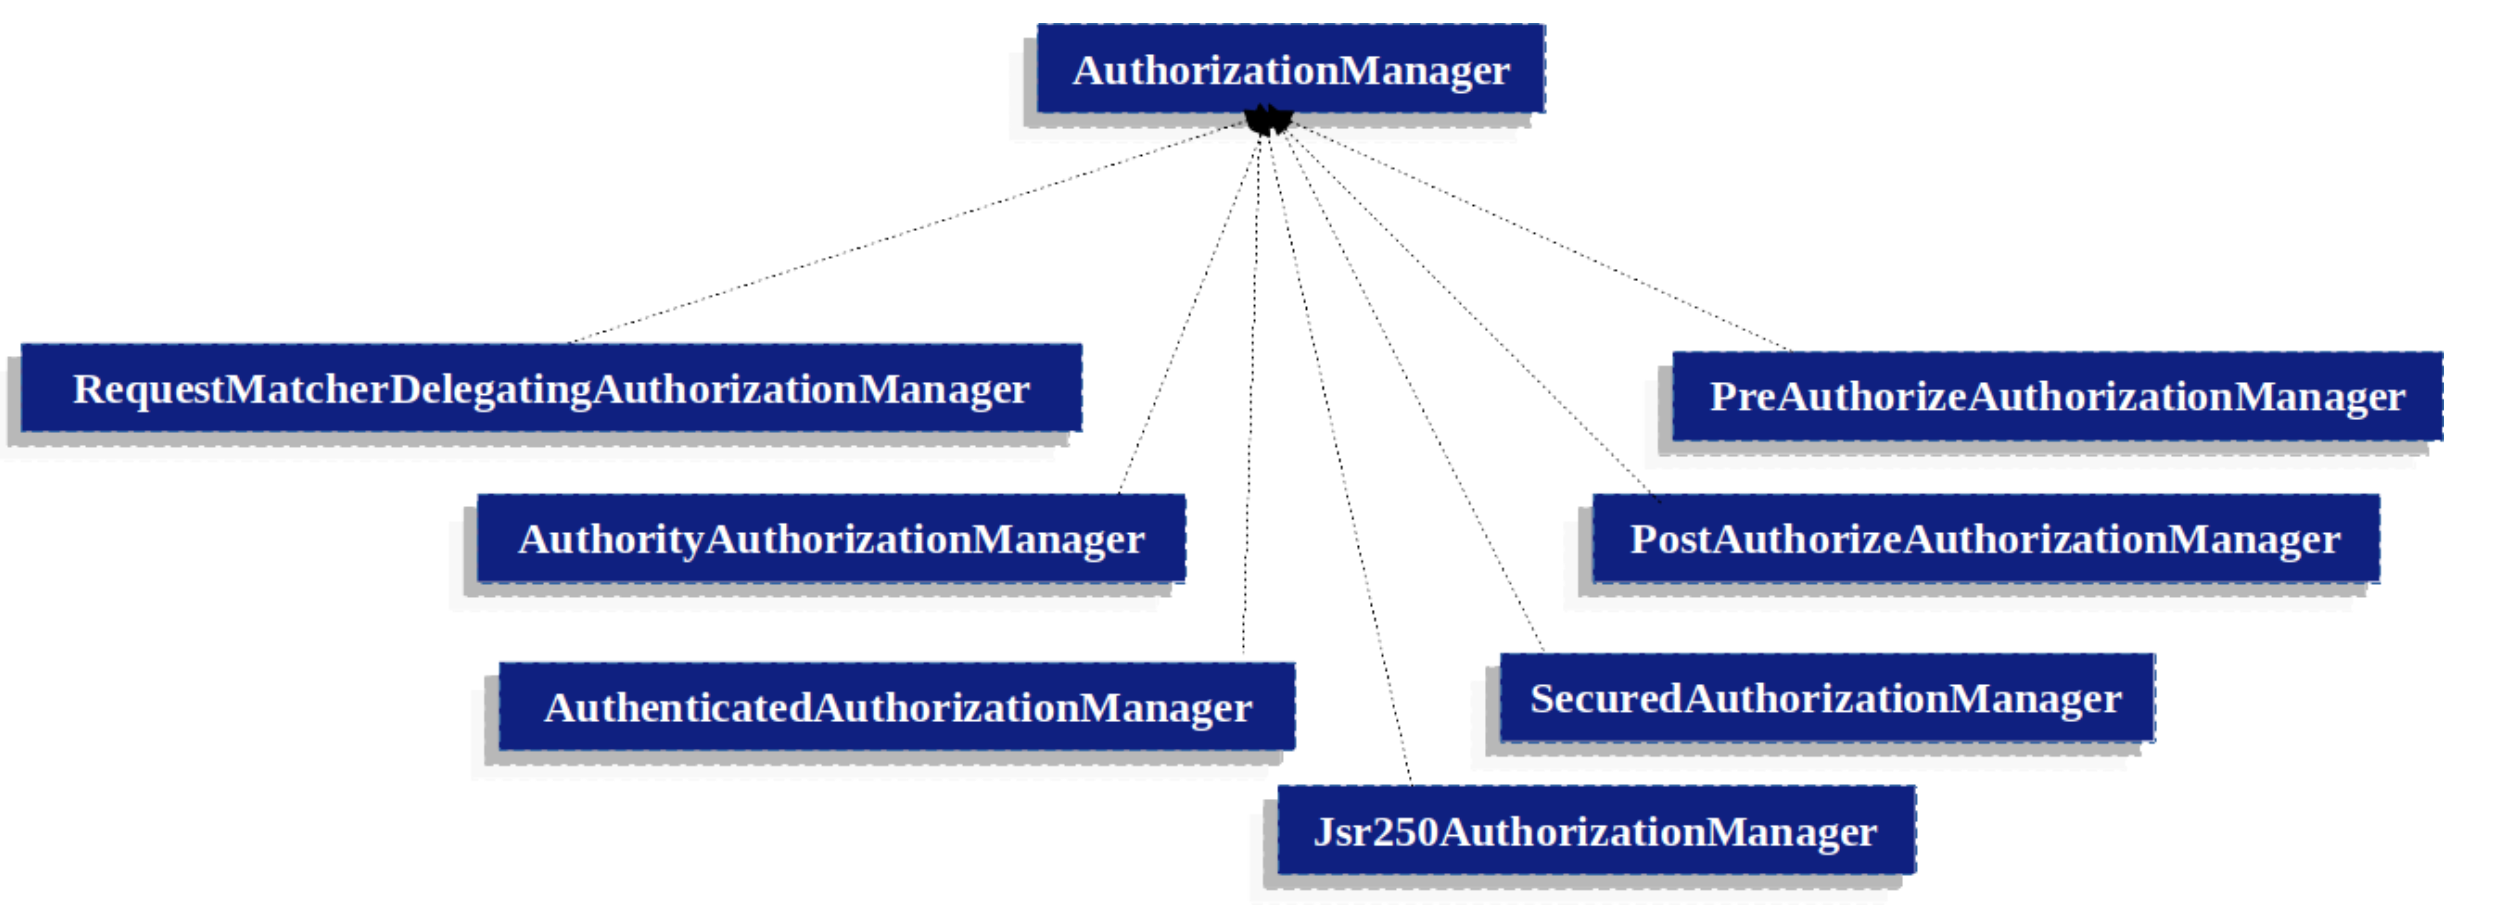
\includegraphics[width=1\linewidth]{auth-manag-impl}
    \caption{Spring Security Filter Chain}
    \label{fig:auth-manag-impl}
\end{figure}

\subsubsection{Method Security}

Spring Security also supports modeling at the method level.

You can activate it in your application by annotating any @Configuration class with @EnableMethodSecurity or adding \textless method-security \textgreater  to any XML configuration file. (Note: Spring Boot Starter Security does not activate method-level authorization by default.)

Then, you are immediately able to annotate any Spring-managed class or method with @PreAuthorize, @PostAuthorize, @PreFilter, and @PostFilter to authorize method invocations, including the input parameters and return values. This is because in the annotation interface \lstinline|EnableMethodSecurity|, the parameter \lstinline|prePostEnabled| is, by default, true.

\paragraph{Pre-Post hooks}

All of @PreFilter, @PostFilter, @PreAuthorize and @PostAuthorize are to be passed SpEL expressions. See interfaces in \lstinline|org.springframework.security.access.prepost:|

\begin{lstlisting}

    // Annotation for specifying a method access-control expression which will be evaluated after a method has been invoked.
    PostAuthorize

    Annotation for specifying a method filtering expression which will be evaluated after a method has been invoked.
    PostFilter

    // Annotation for specifying a method access-control expression which will be evaluated to decide whether a method invocation is allowed or not.
    PreAuthorize

    // Annotation for specifying a method filtering expression which will be evaluated before a method has been invoked.
    PreFilter

\end{lstlisting}

Spring Security’s method authorization support is handy for:

\begin{itemize}
    \item Extracting fine-grained authorization logic; for example, when the method parameters and return values contribute to the authorization decision.
    \item Enforcing security at the service layer.
    \item Stylistically favoring annotation-based over HttpSecurity-based configuration.
\end{itemize}

And since Method Security is built using Spring AOP, you have access to all its expressive power to override Spring Security’s defaults as needed.

Example:

\begin{lstlisting}
   @Service
   public class MyCustomerService {
       @PreAuthorize("hasAuthority('permission:read')")
       @PostAuthorize("returnObject.owner == authentication.name")
       public Customer readCustomer(String id) { ... }
   }
\end{lstlisting}

Note: The @Secured annotation doesn’t support Spring Expression Language (SpEL).

\paragraph{@Secured and @jsr250Enabled}

These parameters to EnableMethodSecurity need to be explicitly enabled.

The \lstinline|@Secured| annotation is used to specify a list of roles on a method.

Example:

\begin{lstlisting}
    @Secured({ "ROLE_VIEWER", "ROLE_EDITOR" })
    public boolean isValidUsername(String username) {
        return userRoleRepository.isValidUsername(username);
    }

\end{lstlisting}

\lstinline|@RolesAllowed| is JSR-250’s equivalent. Example:

\begin{lstlisting}
    @RolesAllowed({ "ROLE_VIEWER", "ROLE_EDITOR" })
    public boolean isValidUsername2(String username) {
        //...
    }
\end{lstlisting}

\section{Testing with Spring}

\subsection{TestContext Framework}

The Spring TestContext Framework (located in the org.springframework.test.context package) provides generic, annotation-driven unit and integration testing support that is agnostic of the testing framework in use.

In addition to generic testing infrastructure, the TestContext framework provides explicit support for JUnit 4, JUnit Jupiter (AKA JUnit 5), and TestNG.

\subsection{Executing SQL Scripts}

Sometimes it is essential to be able to modify the database during integration tests.
Spring provides the following options for executing SQL scripts programmatically within integration test methods:

\begin{itemize}
    \item org.springframework.jdbc.datasource.init.ScriptUtils
    \item org.springframework.jdbc.datasource.init.ResourceDatabasePopulator
    \item org.springframework.test.context.junit4.AbstractTransactionalJUnit4SpringContextTests
    \item org.springframework.test.context.testng.AbstractTransactionalTestNGSpringContextTests
\end{itemize}

\lstinline|ScriptUtils| provides a collection of static utility methods (all called \lstinline|executeSqlScript|) for working with SQL scripts and is mainly intended for internal use within the framework. However, if you require full control over how SQL scripts are parsed and run, ScriptUtils may suit your needs better than some of the other alternatives described later.

\begin{lstlisting}
    // one of 4 overloaded versions
    public static void executeSqlScript(
        Connection connection,
        EncodedResource resource,
        boolean continueOnError,
        boolean ignoreFailedDrops,
        String commentPrefix,
        @Nullable
        String separator,
        String blockCommentStartDelimiter,
        String blockCommentEndDelimiter
    ) throws ScriptException
\end{lstlisting}

\lstinline|ResourceDatabasePopulator| provides an object-based API for programmatically populating, initializing, or cleaning up a database by using SQL scripts defined in external resources. ResourceDatabasePopulator provides options for configuring the character encoding, statement separator, comment delimiters, and error handling flags used when parsing and running the scripts.

\begin{lstlisting}
    //  Populates, initializes, or cleans up a database using SQL scripts defined in external resources.

    public class ResourceDatabasePopulator implements DatabasePopulator

    /*
    Call addScript(org.springframework.core.io.Resource) to add a single SQL script location.
    Call addScripts(org.springframework.core.io.Resource...) to add multiple SQL script locations.
    Consult the setter methods in this class for further configuration options.
    Call populate(java.sql.Connection) or execute(javax.sql.DataSource) to initialize or clean up the database using the configured scripts.
    */

\end{lstlisting}

In addition to the aforementioned mechanisms for running SQL scripts programmatically, you can declare the \lstinline|@Sql| annotation on a test class or test method to configure individual SQL statements or the resource paths to SQL scripts that should be run against a given database before or after an integration test class or test method. Support for @Sql is provided by the \lstinline|SqlScriptsTestExecutionListener|, which is enabled by default.

\subsection{MockMvc}

The Spring MVC Test framework, also known as MockMvc, aims to provide more complete testing for Spring MVC controllers without a running server. It does that by invoking the DispatcherServlet and passing “mock” implementations of the Servlet API from the spring-test module which replicates the full Spring MVC request handling without a running server.

\subsubsection{Implications}

As opposed to @SpringBootTest, MockMvc is built on Servlet API mock implementations from the spring-test module and does not rely on a running container.

MockMvc starts out with a blank MockHttpServletRequest. Whatever is added to it is what the request becomes. There is no jsessionid cookie; no forwarding, error, or async dispatches; and no JSP rendering. Instead, “forwarded” and “redirected” URLs are saved in the MockHttpServletResponse and can be \textit{asserted with expectations}.

This means that, if you use JSPs, you can verify the JSP page to which the request was forwarded, but no HTML is rendered. In other words, the JSP is not invoked. Note, however, that all other rendering technologies that do not rely on forwarding, such as Thymeleaf and Freemarker, render HTML to the response body as expected. The same is true for rendering JSON, XML, and other formats through @ResponseBody methods.

\subsubsection{Static imports}

When using MockMvc directly to perform requests, the following static imports are needed:

\begin{itemize}
    \item MockMvcBuilders.*

    \item MockMvcRequestBuilders.*

    \item MockMvcResultMatchers.*

    \item MockMvcResultHandlers.*
\end{itemize}

\subsubsection{Setup}

MockMvc can be setup in one of two ways. One is to point directly to the controllers you want to test and programmatically configure Spring MVC infrastructure. Example:

\begin{lstlisting}
    class MyWebTests {

        MockMvc mockMvc;

        @BeforeEach
        void setup() {
            this.mockMvc = MockMvcBuilders.standaloneSetup(new AccountController()).build();
        }

        // ...

    }
\end{lstlisting}

The second is to point to Spring configuration with Spring MVC and controller infrastructure in it.

\begin{lstlisting}
    @SpringJUnitWebConfig(locations = "my-servlet-context.xml")
    class MyWebTests {

        MockMvc mockMvc;

        @BeforeEach
        void setup(WebApplicationContext wac) {
            this.mockMvc = MockMvcBuilders.webAppContextSetup(wac).build();
        }

        // ...

    }
\end{lstlisting}

\subsubsection{Queries with MockMvc}

Example queries using MockMvc:

\begin{lstlisting}
    mockMvc.perform(post("/hotels/{id}", 42).accept(MediaType.APPLICATION_JSON));

    // a file upload request that internally uses MockMultipartHttpServletRequest
    mockMvc.perform(multipart("/doc").file("a1", "ABC".getBytes("UTF-8")));

    // specifying query parameters in URI template style
    mockMvc.perform(get("/hotels?thing={thing}", "somewhere"));

    // adding Servlet request parameters that represent either query or form parameters
    mockMvc.perform(get("/hotels").param("thing", "somewhere"));


\end{lstlisting}


\subsection{Mocking in detail: @Mock vs. @MockBean}

@Mock is an annotation provided by the Mockito library. It is used to create mock objects for dependencies that are not part of the Spring context.

The @Mock annotation is typically used in conjunction with the MockitoJUnitRunner or MockitoExtension to initialize the mock objects.

Example:

\begin{lstlisting}
    import static org.mockito.Mockito.*;

    @RunWith(MockitoJUnitRunner.class)
    public class UserServiceTest {

        @Mock
        private UserRepository userRepository;

        // inject mock objects into UserService
        @InjectMocks
        private UserService userService;

        @Test
        public void testGetUserById() {
            // Given
            User mockedUser = new User("John", "Doe", 25);
            when(userRepository.findById(1L)).thenReturn(
            Optional.of(mockedUser));

            // When
            User result = userService.getUserById(1L);

            // Then
            assertNotNull(result);
            assertEquals("John", result.getFirstName());

            // Verify that the findById method was called
            verify(userRepository).findById(1L);
        }
    }
\end{lstlisting}

In contrast, @MockBean is a Spring Boot-specific annotation provided by the Spring Boot Test module. It is used to create mock objects for dependencies that are part of the Spring context.
Example:

\begin{lstlisting}
    @SpringBootTest
    public class UserServiceIntegrationTest {

        @Autowired
        private UserService userService;

        @MockBean
        private UserRepository userRepository;

        @Test
        public void testGetUserById() {
            // same as above
        }
    }
\end{lstlisting}


Key differences:

\begin{itemize}
    \item @Mock can only be applied to fields and parameters, whereas @MockBean can only be applied to classes and fields.
    \item @Mock can be used to mock any Java class or interface while @MockBean only allows for mocking of Spring beans or creation of mock Spring beans. It can be used to mock existing beans, but also to create new beans that will belong to the Spring application context.
    \item To be able to use the @MockBean annotation, the Spring runner (@RunWith(SpringRunner.class) ) is used, whereas @Mock is used with MockitoJUnitRunner.
    \item @MockBean can be used to create custom annotations for specific, reoccurring, needs.
\end{itemize}

Both @Mock and @MockBean are included in spring-boot-starter-test.

\section{Spring Web MVC}

Spring Web MVC is the original web framework built on the Servlet API and has been included in the Spring Framework from the very beginning.

It is packaged in \textit{spring-textmvc.jar}.

\subsection{Controllers}

    @RequestMapping handler methods have a flexible signatu\texttt{}re and can choose from a range of supported controller method arguments and return values.

    Supported controller method arguments are:

    \begin{lstlisting}
    // Generic access to request parameters and request and session attributes, without direct use of the Servlet API.
    WebRequest

    // Choose any specific request or response type -for example, ServletRequest, HttpServletRequest, or Spring's MultipartRequest, MultipartHttpServletRequest.
    jakarta.servlet.ServletRequest, jakarta.servlet.ServletResponse

    jakarta.servlet.http.HttpSession

    java.security.Principal

    HttpMethod

    // Java
    java.util.Locale

    java.util.TimeZone + java.time.ZoneId



    // For access to the raw request body as exposed by the Servlet API.
    java.io.InputStream, java.io.Reader

    // For access to the raw response body as exposed by the Servlet API.
    java.io.OutputStream, java.io.Writer

    @PathVariable
    //For access to name-value pairs in URI path segments.
    @MatrixVariable

    @RequestParam
    // For access to the Servlet request parameters, including multipart files. Parameter values are converted to the declared method argument type.

    // For access to request headers. Header values are converted to the declared method argument type,
    @RequestHeader

    @CookieValue

    // For access to the HTTP request body. Body content is converted to the declared method argument type by using HttpMessageConverter implementations.
    @RequestBody

    // For access to request headers and body. The body is converted with an HttpMessageConverter.
    HttpEntity<B>

    // For access to a part in a multipart/form-data request, converting the part's body with an HttpMessageConverter.
    @RequestPart

    // For access to the model that is used in HTML controllers and exposed to templates as part of view rendering.
    java.util.Map, org.springframework.ui.Model, org.springframework.ui.ModelMap

    // Attributes to use in case of a redirect (that is, to be appended to the query string) and flash attributes to be stored temporarily until the request after redirect.
    RedirectAttributes

    // For access to an existing attribute in the model (instantiated if not present) with data binding and validation applied. See @ModelAttribute as well as Model and DataBinder.
    @ModelAttribute

    // For access to errors from validation and data binding for a command object (that is, a @ModelAttribute argument) or errors from the validation of a @RequestBody or @RequestPart arguments.
    Errors, BindingResult

    // For preparing a URL relative to the current request's host, port, scheme, context path, and the literal part of the servlet mapping. See URI Links.
    UriComponentsBuilder

    // For access to any session attribute, in contrast to model attributes stored in the session as a result of a class-level @SessionAttributes declaration.
    @SessionAttribute

    @RequestAttribute

    // If a method argument is not matched to any of the earlier values in this table and it is a simple type (as determined by BeanUtils#isSimpleProperty), it is resolved as a @RequestParam. Otherwise, it is resolved as a @ModelAttribute.
    \end{lstlisting}

    Supported return values \textit{include}:

    \begin{lstlisting}
    // The return value is converted through HttpMessageConverter implementations and written to the response.
    @ResponseBody

    // The return value that specifies the full response (including HTTP headers and body) is to be converted through HttpMessageConverter implementations and written to the response.
    HttpEntity<B>, ResponseEntity<B>

    HttpHeaders

    ErrorResponse

    // A view name to be resolved with ViewResolver implementations and used together with the implicit model
    String

    //  A View instance to use for rendering together with the implicit model
    View

    // The view and model attributes to use and, optionally, a response status.
    ModelAndView

    // Attributes to be added to the implicit model, with the view name implicitly determined through a RequestToViewNameTranslator.
    org.springframework.ui.Model
    java.util.Map
    \end{lstlisting}

\subsection{Securing Endpoints}

To enable Spring Security integration with Spring MVC, add the \lstinline|@EnableWebSecurity| annotation to your configuration.

Configuring HTTP security using \lstinline|HttpSecurity| in a class extending \lstinline|WebSecurityConfigurerAdapter| allows you to define security rules for your application, such as requiring authentication for certain endpoints.

Example:

\begin{lstlisting}
    @Configuration
    @EnableWebSecurity
    public class SecurityConfig extends WebSecurityConfigurerAdapter {

        @Override
        protected void configure(HttpSecurity http) throws Exception {
            http
            .authorizeRequests()
            .antMatchers("/public/**").permitAll()
            .anyRequest().authenticated()
            .and()
            .formLogin().permitAll()
            .and()
            .logout().permitAll();
        }
    }
\end{lstlisting}

Spring Security provides deep integration with how Spring MVC matches on URLs with MvcRequestMatcher. This is helpful to ensure that your Security rules match the logic used to handle your requests.
Consider a controller that is mapped as follows:

\begin{lstlisting}
    @RequestMapping("/admin")
    public String admin() {
        // ...
    }
\end{lstlisting}

To restrict access to this controller method to admin users, you can provide authorization rules by matching on the HttpServletRequest with the following:

\begin{lstlisting}
   @Bean
   public SecurityFilterChain filterChain(HttpSecurity http) throws Exception {
       http
       .authorizeHttpRequests((authorize) -> authorize
       .requestMatchers("/admin").hasRole("ADMIN")
       );
       return http.build();
   }

\end{lstlisting}

With either configuration, the /admin URL requires the authenticated user to be an admin user. However, depending on our Spring MVC configuration, the /admin.html URL also maps to our admin() method. Additionally, depending on our Spring MVC configuration, the /admin URL also maps to our admin() method.

The problem is that our security rule protects only /admin. We could add additional rules for all the permutations of Spring MVC, but this would be quite verbose and tedious.

Fortunately, when using the requestMatchers DSL method, Spring Security automatically creates a MvcRequestMatcher if it detects that Spring MVC is available in the classpath. Therefore, it will protect the same URLs that Spring MVC will match on by using Spring MVC to match on the URL.

\subsection{Type Conversion}

By default, formatters for various number and date types are installed, along with support for customization via @NumberFormat, @DurationFormat, and @DateTimeFormat on fields and parameters.

To register custom formatters and converters, use the following:

\begin{lstlisting}
    @Configuration
    public class WebConfiguration implements WebMvcConfigurer {

        @Override
        public void addFormatters(FormatterRegistry registry) {
            // ...
        }
    }
\end{lstlisting}

\begin{lstlisting}
\end{lstlisting}

\subsection{Validation}

JSR-303/JSR-380 annotations provide a standard way of validating objects in Java. These annotations can be used on domain object fields to enforce validation constraints.

Example:

\begin{lstlisting}
    public class User {

        @NotNull
        @Size(min = 1, max = 20)
        private String name;
    }
\end{lstlisting}

In addition, if Bean Validation is present on the classpath (for example, Hibernate Validator), the LocalValidatorFactoryBean is registered as a global Validator for use with @Valid and @Validated on controller method arguments.

You can customize the global Validator instance, as the following example shows:

\begin{lstlisting}
    @Configuration
    public class WebConfiguration implements WebMvcConfigurer {

        @Override
        public Validator getValidator() {
            Validator validator = new OptionalValidatorFactoryBean();
            // ...
            return validator;
        }
    }
\end{lstlisting}

Note that you can also register Validator implementations locally, as the following example shows:

\begin{lstlisting}
    @Controller
    public class MyController {

        @InitBinder
        public void initBinder(WebDataBinder binder) {
            binder.addValidators(new FooValidator());
        }
    }

\end{lstlisting}

\subsection{Interceptors}

You can register interceptors to apply to incoming requests, as the following example shows:

\begin{lstlisting}
    @Configuration
    public class WebConfiguration implements WebMvcConfigurer {

        @Override
        public void addInterceptors(InterceptorRegistry registry) {
            registry.addInterceptor(new LocaleChangeInterceptor());
        }
    }
\end{lstlisting}

\subsection{Filters}

Implementing the Filter interface and registering it as a bean allows you to define custom behavior for each HTTP request. The filter will be applied to all incoming requests.

Example:


\begin{lstlisting}
    @Component
public class RequestLoggingFilter implements Filter {

    @Override
    public void doFilter(ServletRequest request, ServletResponse response, FilterChain chain)
    throws IOException, ServletException {
        // Log request details
        chain.doFilter(request, response);
    }
}
\end{lstlisting}

\subsection{Content Types}

You can configure how Spring MVC determines the requested media types from the request (for example, Accept header, URL path extension, query parameter, and others).

By default, only the Accept header is checked.

You can customize requested content type resolution, as the following example shows:

\begin{lstlisting}
    @Configuration
    public class WebConfiguration implements WebMvcConfigurer {

        @Override
        public void configureContentNegotiation(
        ContentNegotiationConfigurer configurer) {
            configurer.mediaType("json", MediaType.APPLICATION_JSON);
            configurer.mediaType("xml", MediaType.APPLICATION_XML);
        }
    }
\end{lstlisting}

\subsection{Message Converters}

You can set the HttpMessageConverter instances to use in Java configuration, replacing the ones used by default, by overriding configureMessageConverters(). You can also customize the list of configured message converters at the end by overriding extendMessageConverters().

In a Spring Boot application, the WebMvcAutoConfiguration adds any HttpMessageConverter beans it detects, in addition to default converters. Hence, in a Boot application, prefer to use the HttpMessageConverters mechanism.

Or alternatively, use extendMessageConverters to modify message converters at the end.

The following example adds XML and Jackson JSON converters with a customized ObjectMapper instead of the default ones:

\begin{lstlisting}
    @Configuration
    public class WebConfiguration implements WebMvcConfigurer {

        @Override
        public void configureMessageConverters(
        List<HttpMessageConverter<?>> converters) {
            Jackson2ObjectMapperBuilder builder = new Jackson2ObjectMapperBuilder()
            .indentOutput(true)
            .dateFormat(new SimpleDateFormat("yyyy-MM-dd"))
            .modulesToInstall(new ParameterNamesModule());
            converters.add(new MappingJackson2HttpMessageConverter(
            builder.build()));
            converters.add(new MappingJackson2XmlHttpMessageConverter(
            builder.createXmlMapper(true).build()));
        }
    }
\end{lstlisting}

\subsection{HTTP Message Conversion}

The spring-web module contains the HttpMessageConverter interface for reading and writing the body of HTTP requests and responses through InputStream and OutputStream. HttpMessageConverter instances are used on the client side (for example, in the RestClient) and on the server side (for example, in Spring MVC REST controllers).

Concrete implementations for the main media (MIME) types are provided in the framework and are, by default, registered with the RestClient and RestTemplate on the client side and with RequestMappingHandlerAdapter on the server side (see Configuring Message Converters).

Some implementations of HttpMessageConverter are:

    \begin{lstlisting}
    StringHttpMessageConverter
    FormHttpMessageConverter
    ByteArrayHttpMessageConverter
    MarshallingHttpMessageConverter
    JsonbHttpMessageConverter
    ProtobufHttpMessageConverter
    ProtobufJsonFormatHttpMessageConverter
    \end{lstlisting}

\subsection{URI Links}

\subsubsection{UriComponents}

UriComponentsBuilder helps to build URI’s from URI templates with variables.

\begin{lstlisting}
    UriComponents uriComponents = UriComponentsBuilder
    .fromUriString("https://example.com/hotels/{hotel}")
    .queryParam("q", "{q}")
    .encode()
    .build();

    URI uri = uriComponents.expand("Westin", "123").toUri();
\end{lstlisting}

The preceding example can be consolidated into one chain and shortened with buildAndExpand:

\begin{lstlisting}
    URI uri = UriComponentsBuilder
    .fromUriString("https://example.com/hotels/{hotel}")
    .queryParam("q", "{q}")
    .encode()
    .buildAndExpand("Westin", "123")
    .toUri();

\end{lstlisting}

You can shorten it further by going directly to a URI (which implies encoding):

\begin{lstlisting}
    URI uri = UriComponentsBuilder
    .fromUriString("https://example.com/hotels/{hotel}")
    .queryParam("q", "{q}")
    .build("Westin", "123");

\end{lstlisting}

You can shorten it further still with a full URI template:

\begin{lstlisting}
    URI uri = UriComponentsBuilder
    .fromUriString("https://example.com/hotels/{hotel}?q={q}")
    .build("Westin", "123");
\end{lstlisting}

\subsubsection{UriBuilder}

UriComponentsBuilder implements UriBuilder. You can create a UriBuilder, in turn, with a UriBuilderFactory. Together, UriBuilderFactory and UriBuilder provide a pluggable mechanism to build URIs from URI templates, based on shared configuration, such as a base URL, encoding preferences, and other details.

You can configure RestTemplate and WebClient with a UriBuilderFactory to customize the preparation of URIs. DefaultUriBuilderFactory is a default implementation of UriBuilderFactory that uses UriComponentsBuilder internally and exposes shared configuration options.

The following example shows how to configure a RestTemplate:
\begin{lstlisting}
    // import org.springframework.web.util.
        DefaultUriBuilderFactory.EncodingMode;

    String baseUrl = "https://example.org";
    DefaultUriBuilderFactory factory = new DefaultUriBuilderFactory(baseUrl);
    factory.setEncodingMode(EncodingMode.TEMPLATE_AND_VALUES);

    RestTemplate restTemplate = new RestTemplate();
    restTemplate.setUriTemplateHandler(factory);

    In addition, you can also use DefaultUriBuilderFactory directly. It is similar to using UriComponentsBuilder but, instead of static factory methods, it is an actual instance that holds configuration and preferences.

    String baseUrl = "https://example.com";
    DefaultUriBuilderFactory uriBuilderFactory = new DefaultUriBuilderFactory(baseUrl);

    URI uri = uriBuilderFactory.uriString("/hotels/{hotel}")
    .queryParam("q", "{q}")
    .build("Westin", "123");
\end{lstlisting}

\subsection{View Controllers}

This is a shortcut for defining a ParameterizableViewController that immediately forwards to a view when invoked. You can use it in static cases when there is no Java controller logic to run before the view generates the response.

The following example forwards a request for / to a view called home:

\begin{lstlisting}
    @Configuration
    public class WebConfiguration implements WebMvcConfigurer {

        @Override
        public void addViewControllers(ViewControllerRegistry registry) {
            registry
            .addViewController("/")
            .setViewName("home");
        }
    }
\end{lstlisting}

\subsection{View Resolvers}

The MVC configuration simplifies the registration of view resolvers.

The following example configures content negotiation view resolution by using JSP and Jackson as a default View for JSON rendering:

\begin{lstlisting}
    @Configuration
    public class WebConfiguration implements WebMvcConfigurer {

        @Override
        public void configureViewResolvers(ViewResolverRegistry registry) {
            registry.enableContentNegotiation(new MappingJackson2JsonView());
            registry.jsp();
        }
    }
\end{lstlisting}

\subsection{Template Engines}

As well as REST web services, you can also use Spring MVC to serve dynamic HTML content. Spring MVC supports a variety of templating technologies, including Thymeleaf, FreeMarker, and JSPs. Also, many other templating engines include their own Spring MVC integrations.

Spring Boot includes auto-configuration support for the following templating engines:

\begin{itemize}
    \item FreeMarker
    \item Groovy
    \item Thymeleaf
    \item Mustache
\end{itemize}

If possible, JSPs should be avoided. There are several known limitations when using them with embedded servlet containers.

When you use one of these templating engines with the default configuration, your templates are picked up automatically from src/main/resources/templates.

\subsection{MVC Config}

The MVC Java configuration and the MVC XML namespace provide default configuration suitable for most applications and a configuration API to customize it.

You can use the @EnableWebMvc annotation to enable MVC configuration with programmatic configuration, or \textless mvc:annotation-driven \textgreater  with XML configuration:

\begin{lstlisting}
    @Configuration
    @EnableWebMvc
    public class WebConfiguration {
    }
\end{lstlisting}

The preceding example registers a number of Spring MVC infrastructure beans and adapts to dependencies available on the classpath (for example, payload converters for JSON, XML, and others).

\subsection{MVC Config API}

In Java configuration, you can implement the WebMvcConfigurer interface:

\begin{lstlisting}@Configuration
    public class WebConfiguration implements WebMvcConfigurer {

        // Implement configuration methods...
    }
\end{lstlisting}

\section{REST Clients}

\begin{itemize}
    \item RestClient is a synchronous HTTP client that exposes a modern, fluent API.
    \item WebClient is a reactive client to perform HTTP requests with a fluent API.
    \item RestTemplate is a synchronous client to perform HTTP requests. It is the original Spring REST client and exposes a simple, template-method API over underlying HTTP client libraries.
    \item HTTP Interface: The Spring Frameworks lets you define an HTTP service as a Java interface with HTTP exchange methods. You can then generate a proxy that implements this interface and performs the exchanges. This helps to simplify HTTP remote access and provides additional flexibility for to choose an API style such as synchronous or reactive.
\end{itemize}

Here, we zoom in on RestTemplate.

The RestTemplate provides a high-level API over HTTP client libraries in the form of a classic Spring Template class. It exposes the following groups of overloaded methods:

\begin{lstlisting}
// Retrieves a representation via GET.
getForObject

// Retrieves a ResponseEntity (that is, status, headers, and body) by using GET.
getForEntity

headForHeaders

// Creates a new resource by using POST and returns the Location header from the response.
postForLocation

// Creates a new resource by using POST and returns the representation from the response.
postForObject

// Creates a new resource by using POST and returns the representation from the response.
postForEntity

put

patchForObject

delete

optionsForAllow

// More generalized (and less opinionated) version of the preceding methods that provides extra flexibility when needed. It accepts a RequestEntity (including HTTP method, URL, headers, and body as input) and returns a ResponseEntity.
exchange

// The most generalized way to perform a request, with full control over request preparation and response extraction through callback interfaces.
execute
\end{lstlisting}

RestTemplate uses the same HTTP library abstraction as RestClient. By default, it uses the SimpleClientHttpRequestFactory, but this can be changed via the constructor.

RestTemplate can be instrumented for observability, in order to produce metrics and traces.

Objects passed into and returned from RestTemplate methods are converted to and from HTTP messages with the help of an HttpMessageConverter.

\section{Integration Features}

\subsection{Task Execution and Scheduling}
Spring provides annotation support for both task scheduling and asynchronous method execution.

To enable support for @Scheduled and @Async annotations, you can add @EnableScheduling and @EnableAsync to one of your @Configuration classes, or \textless task:annotation-driven \textgreater element:

\begin{lstlisting}
    @Configuration
    @EnableAsync
    @EnableScheduling
    public class SchedulingConfiguration {
    }

\end{lstlisting}

@Scheduled usage example:

\begin{lstlisting}
    @Scheduled(fixedDelay = 5000)
    public void doSomething() {
        // something that should run periodically
    }
\end{lstlisting}

\section{Spring Boot (Web): Servlet Web Applications}

If you want to build servlet-based web applications, you can take advantage of Spring Boot’s auto-configuration for Spring MVC or Jersey.

The \textit{Spring Web MVC framework} (cf. fig. \ref{fig:spring-web}) is a rich “model view controller” web framework.
Spring MVC lets you create special @Controller or @RestController beans to handle incoming HTTP requests. Methods in your controller are mapped to HTTP by using @RequestMapping annotations.

\begin{figure}[h]
    \centering
    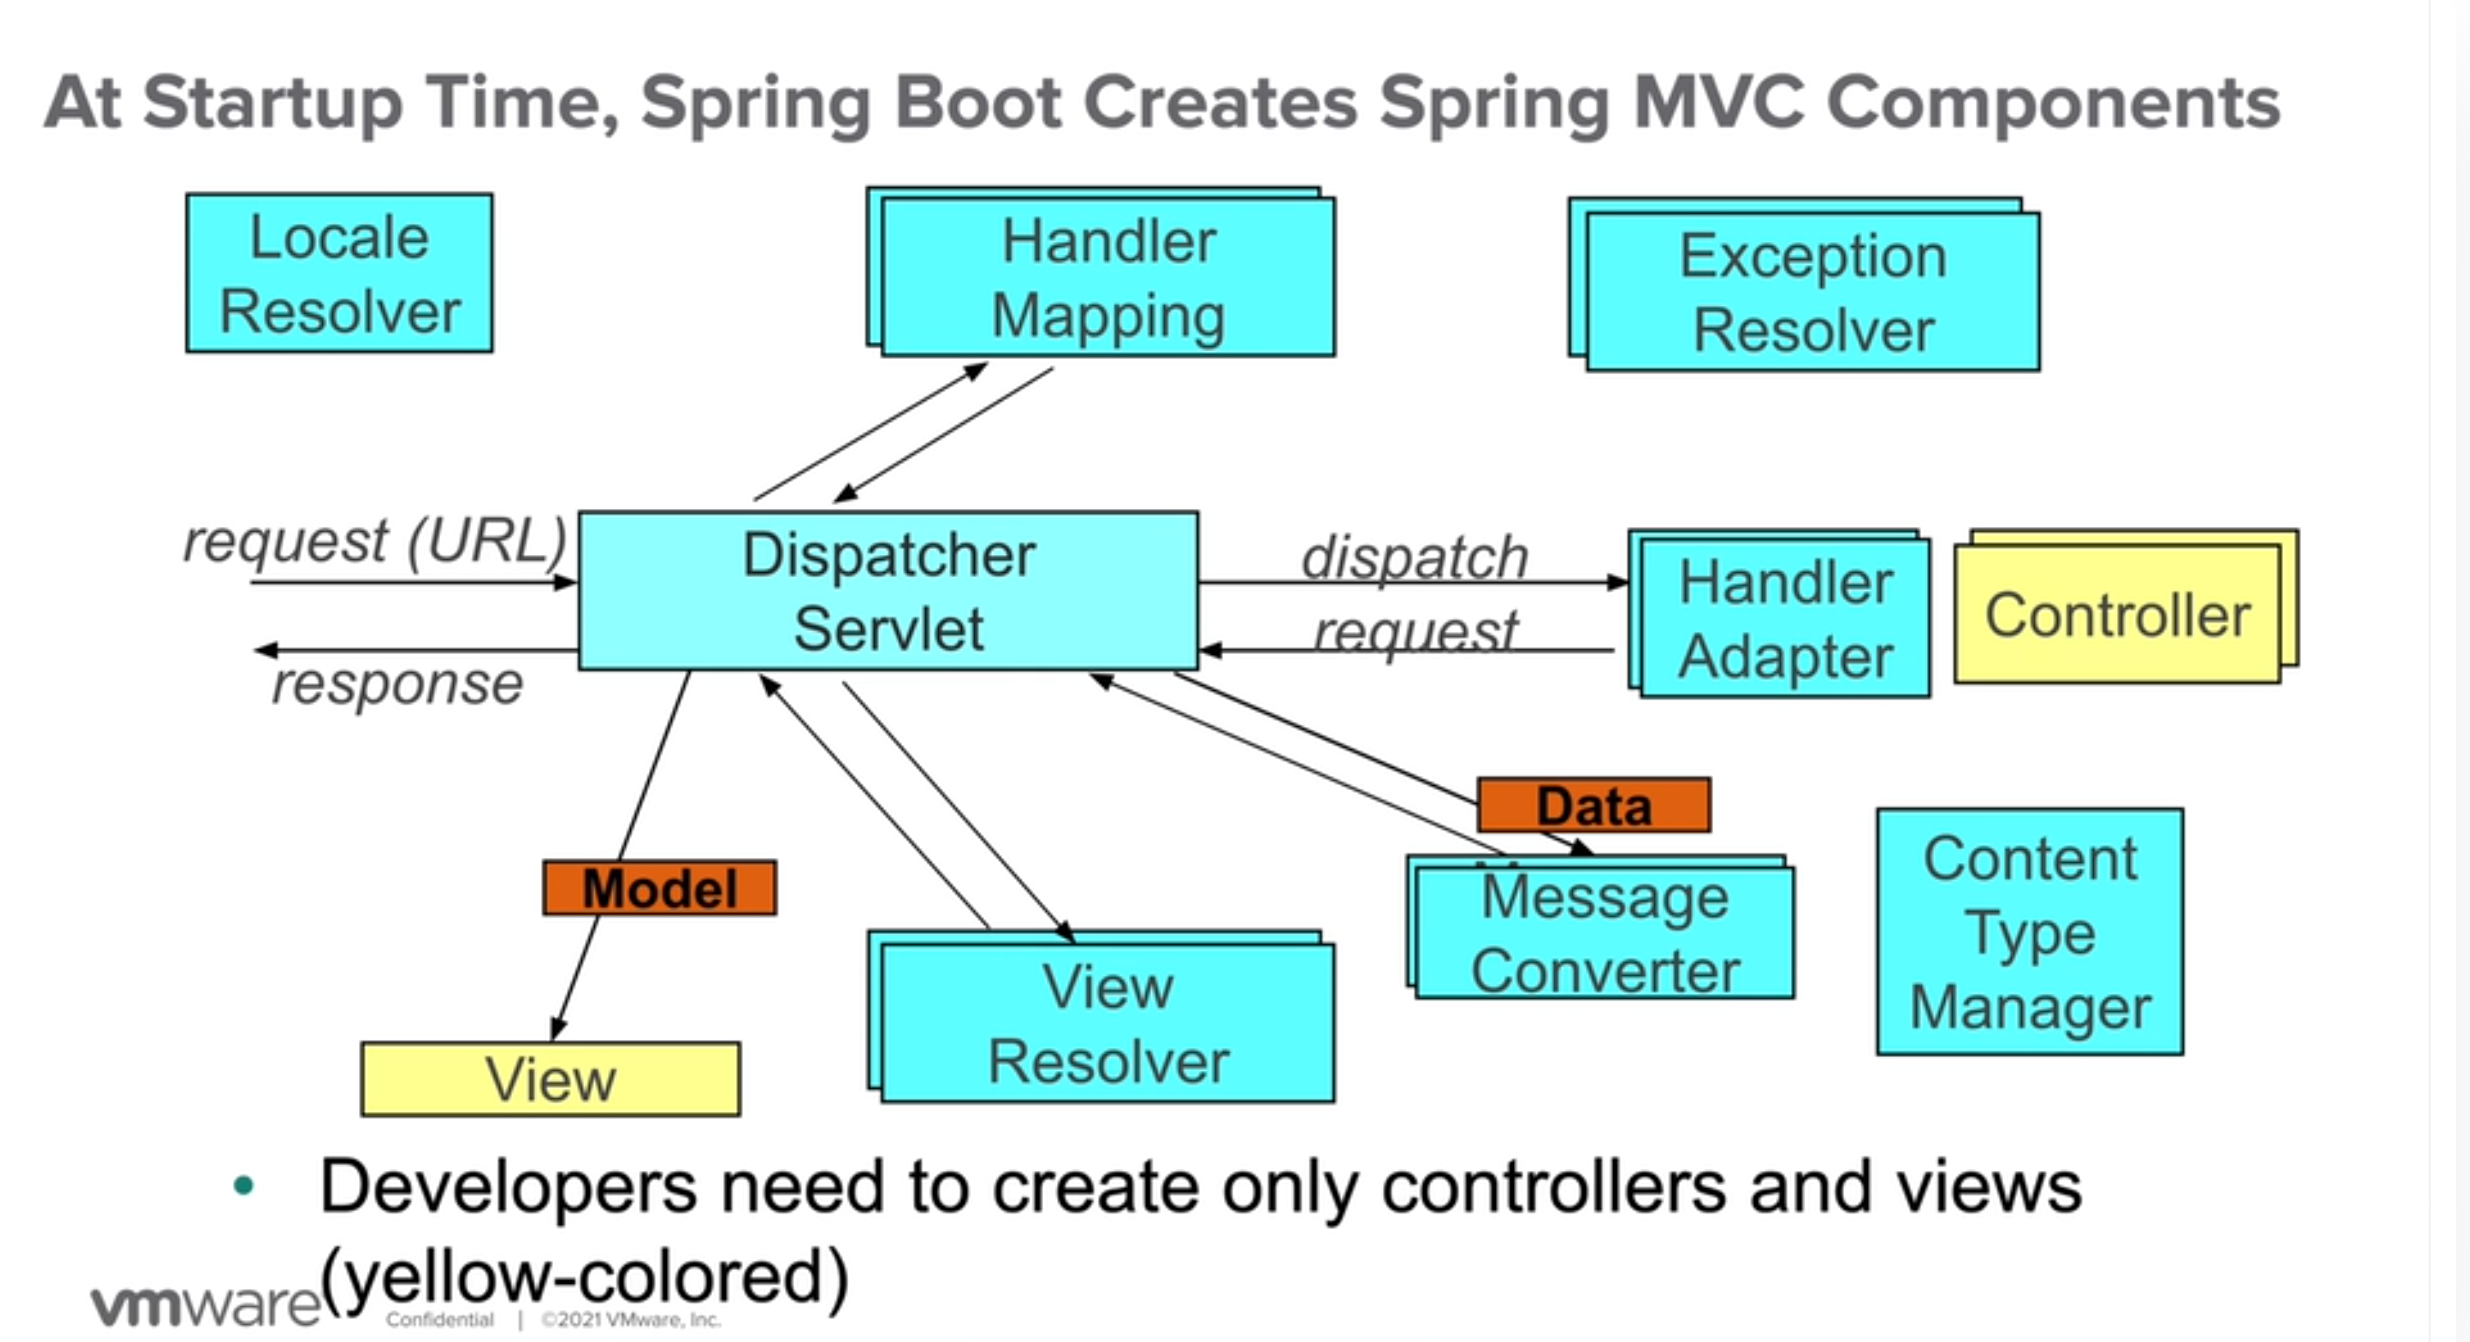
\includegraphics[width=1\linewidth]{spring-web}
    \caption{Spring Boot Web Architecture Overview}
    \label{fig:spring-web}
\end{figure}

Spring Boot provides auto-configuration for Spring MVC that works well with most applications. It replaces the need for @EnableWebMvc, and the two cannot be used together. In addition to Spring MVC’s defaults, the auto-configuration provides the following features:

\begin{itemize}
    \item \lstinline|ContentNegotiatingViewResolver| and \lstinline|BeanNameViewResolver| beans.
    \item Support for serving static resources, including support for WebJars (covered later in this document).
    \item Automatic registration of Converter, GenericConverter, and Formatter beans.
    \item Support for HttpMessageConverters (covered later in this document).
    \item Automatic registration of \lstinline|MessageCodesResolver|.
    \item Static index.html support.
    \item Automatic use of a \lstinline|ConfigurableWebBindingInitializer| bean
\end{itemize}

\subsection{Spring Boot Starters}

Main starter:

\begin{lstlisting}
    // spring-boot-starter/build.gradle

    plugins {
        id "org.springframework.boot.starter"
    }

    description = "Core starter, including auto-configuration support, logging and YAML"

    dependencies {
        api(project(":spring-boot-project:spring-boot"))
        api(project(":spring-boot-project:
        spring-boot-autoconfigure"))
        api(project(":spring-boot-project:
        spring-boot-starters:spring-boot-starter-logging"))
        api("jakarta.annotation:jakarta.annotation-api")
        api("org.springframework:spring-core")
        api("org.yaml:snakeyaml")
    }
\end{lstlisting}

Examples:

\begin{lstlisting}
    // spring-boot-starter-test/build.gradle

    plugins {
        id "org.springframework.boot.starter"
    }

    description = "Starter for testing Spring Boot applications with libraries including JUnit Jupiter, Hamcrest and Mockito"

    dependencies {
        api(project(":spring-boot-project:spring-boot-starters:
        spring-boot-starter"))
        api(project(":spring-boot-project:spring-boot-test"))
        api(project(":spring-boot-project:
        spring-boot-test-autoconfigure"))
        api("com.jayway.jsonpath:json-path")
        api("jakarta.xml.bind:jakarta.xml.bind-api")
        api("net.minidev:json-smart")
        api("org.assertj:assertj-core")
        api("org.awaitility:awaitility")
        api("org.hamcrest:hamcrest")
        api("org.junit.jupiter:junit-jupiter")
        api("org.mockito:mockito-core")
        api("org.mockito:mockito-junit-jupiter")
        api("org.skyscreamer:jsonassert")
        api("org.springframework:spring-core")
        api("org.springframework:spring-test")
        api("org.xmlunit:xmlunit-core") {
            exclude group: "javax.xml.bind", module: "jaxb-api"
        }
    }

    checkRuntimeClasspathForConflicts {
        ignore { name -> name.startsWith("mockito-extensions/") }
    }
\end{lstlisting}
\begin{lstlisting}
    // spring-boot-starter-data-jpa/build.gradle

    plugins {
        id "org.springframework.boot.starter"
    }

    description = "Starter for using Spring Data JPA with Hibernate"

    dependencies {
        api(project(":spring-boot-project:spring-boot-starters:
        spring-boot-starter"))
        api(project(":spring-boot-project:spring-boot-starters:

        spring-boot-starter-jdbc"))
        api("org.hibernate.orm:hibernate-core")
        api("org.springframework.data:spring-data-jpa")
        api("org.springframework:spring-aspects")
    }
\end{lstlisting}
\begin{lstlisting}
    // spring-boot-starter-aop/build.gradle

    plugins {
        id "org.springframework.boot.starter"
    }

    description = "Starter for aspect-oriented programming with Spring AOP and AspectJ"

    dependencies {
        api(project(":spring-boot-project:spring-boot-starters:
        spring-boot-starter"))
        api("org.springframework:spring-aop")
        api("org.aspectj:aspectjweaver")
    }
\end{lstlisting}

Spring Boot provides integration with three JSON mapping libraries: Gson, Jackson, and JSON-B.

Jackson is the preferred and default library.

\subsection{Logging in Spring Boot}

Spring Boot uses \textit{Commons Logging} for all internal logging but leaves the underlying log implementation open.

Default configurations are provided for \textit{Java Util Logging}, \textit{Log4j2}, and \textit{Logback}. In each case, loggers are pre-configured to use console output with optional file output also available.

By default, if you use the starters, \textit{Logback} is used for logging. Appropriate Logback routing is also included to ensure that dependent libraries that use Java Util Logging, Commons Logging, Log4J, or SLF4J all work correctly.

The default log level used by Spring Boot is INFO.
\subsection{SpringApplication}

In addition to the usual Spring Framework events, such as ContextRefreshedEvent, a SpringApplication sends some additional application events.

Some events are actually triggered before the ApplicationContext is created, so you cannot register a listener on those as a @Bean. You can register them with the \lstinline|SpringApplication.addListeners...)| method or the \lstinline|SpringApplicationBuilder.listeners(...)| method.

If you want those listeners to be registered automatically, regardless of the way the application is created, you can add a \lstinline|META-INF/spring.factories| file to your project and reference your listener(s) by using the ApplicationListener key, as shown in the following example:

\begin{lstlisting}
    org.springframework.context.ApplicationListener = com.example.project.MyListener
\end{lstlisting}

A Spring Boot application can be shut down programmatically in the following ways:
\begin{itemize}
    \item use \lstinline|AbstractApplicationContext.close()|
    \item call \lstinline|SpringApplication.exit()|
    \item register a shutdown hook: \lstinline|AbstractApplicationContext.registerShutdownHook()|
    \item use Actuator (need to enable the shutdown endpoint)
\end{itemize}

\subsection{More on spring.factories}

The spring.factories file can be used to register custom interface implementations in the following cases:

\begin{itemize}
    \item Register application event listeners regardless of how the Spring Boot application is created (configured). This is done by implementing a class that inherits from SpringApplicationEvent.
    \item Locate auto-configuration candidates in, for instance, your own starter module.
    \item Register a filter to limit the auto-configuration classes considered. See AutoConfigurationImportFilter.
    \item  Activate application listeners that create a file containing the application process id and/or create file(s) containing the port number(s) used by the running web server (if any). These listeners, ApplicationPidFileWriter and WebServerPortFileWriter, both implement the ApplicationListener interface.
    \item Register failure analyzers. Failure analyzers implement the FailureAnalyzer interface.
    \item Customize the environment or application context prior to Spring Boot application startup, by implementing the ApplicationListener, ApplicationContextListener or the EnvironmentPostProcessor interfaces.
    \item Register the availability of view template providers. See TemplateAvailabilityProvider interface.
\end{itemize}
\subsection{ApplicationContext in Boot}

A SpringApplication attempts to create the right type of ApplicationContext on your behalf. The algorithm used to determine a WebApplicationType is the following:

\begin{itemize}
    \item If Spring MVC is present, an AnnotationConfigServletWebServerApplicationContext is used.
    \item If Spring MVC is not present and Spring WebFlux is present, an AnnotationConfigReactiveWebServerApplicationContext is used.
    \item Otherwise, AnnotationConfigApplicationContext is used.
\end{itemize}

It is also possible to take complete control of the ApplicationContext type that is used by calling setApplicationContextFactory(...).


Architecture Overview (see \ref{fig:spring-web}):

\begin{figure}[h]
    \centering
    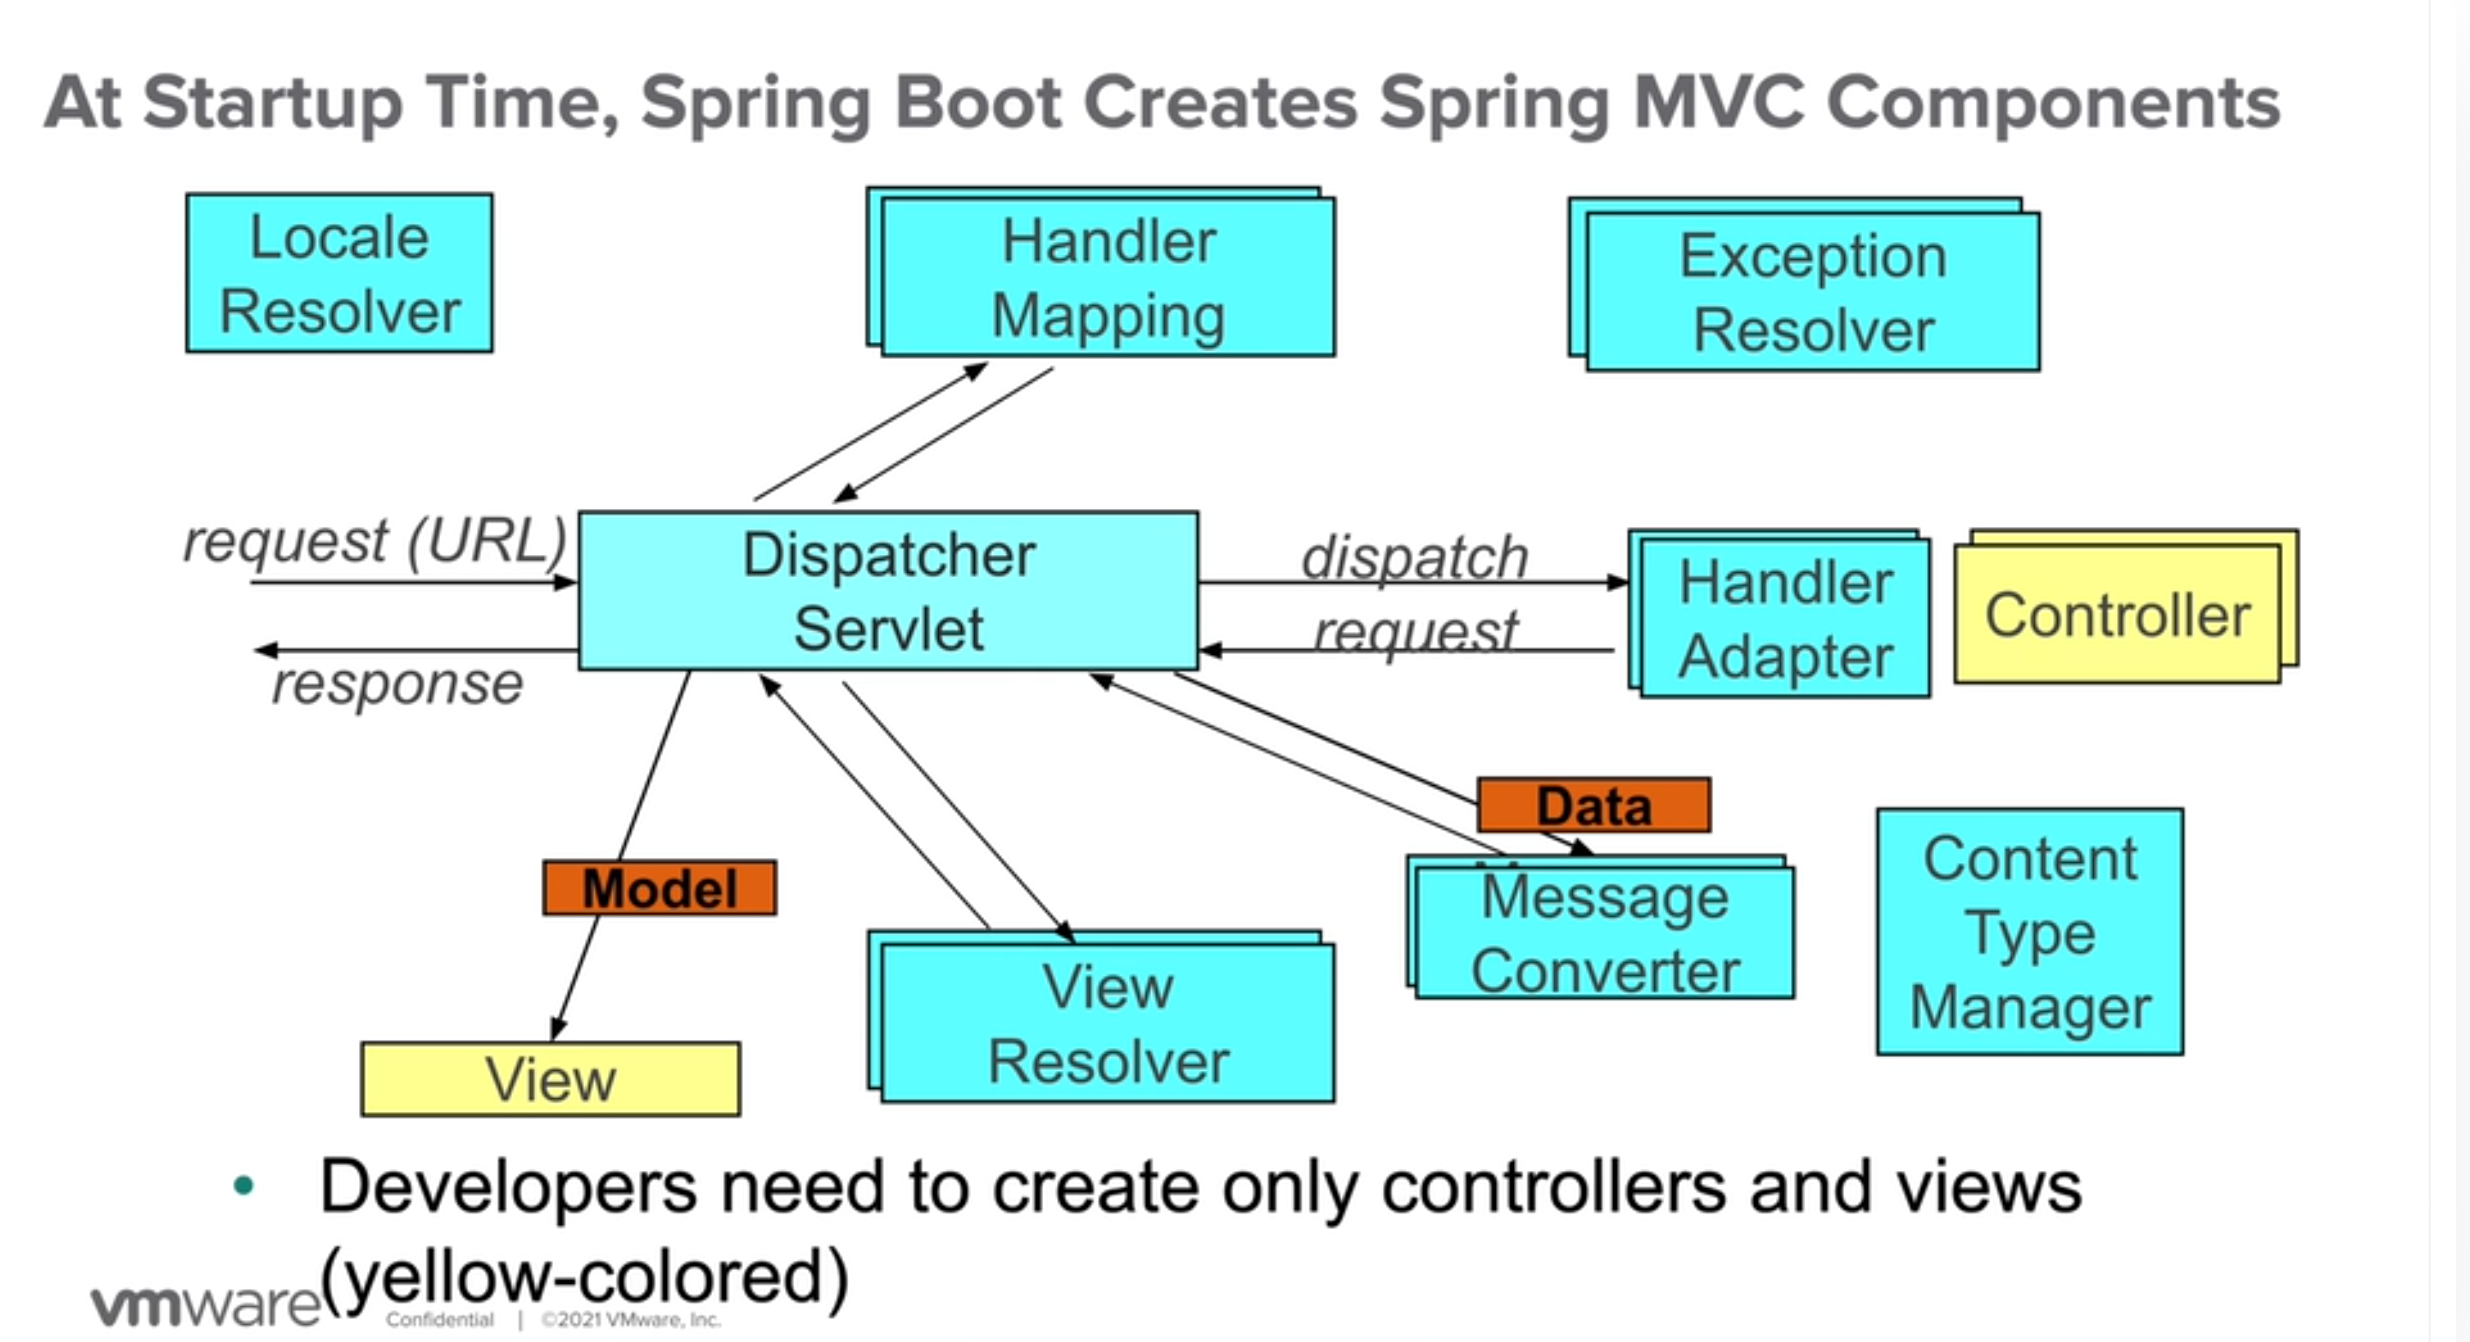
\includegraphics[width=1\linewidth]{spring-web}
    \caption{Spring Boot Web Architecture Overview}
    \label{fig:spring-web}
\end{figure}

\subsection{Accessing Command Line Properties}

By default, SpringApplication converts any command line option arguments (that is, arguments
starting with \lstinline|--|, such as \lstinline|--server.port=9000)| to a property and adds them to the Spring Environment.
Command line properties always take precedence over file-based
property sources.

If you do not want command line properties to be added to the Environment, you can disable them
by using \lstinline|SpringApplication.setAddCommandLineProperties(false)|.

\subsection{Externalized Configuration}

Spring Boot lets you externalize your configuration so that you can work with the same application code in different environments. You can use a variety of external configuration sources including Java properties files, YAML files, environment variables, and command-line arguments.

Property values can be injected directly into your beans by using the \lstinline |@Value| annotation, accessed through Spring’s Environment abstraction, or be bound to \textit{structured objects} through \lstinline[]|@ConfigurationProperties|.

Differences between both are:

\begin{itemize}
    \item @ConfigurationProperties does support relaxed binding, allowing for more flexibility in property names and values. On the other hand, @Value does not have this feature, requiring an exact match between the property name and the field.
    \item @ConfigurationProperties can be validated using JSR-303 bean validation, providing a way to enforce constraints on the properties being bound. In contrast, @Value does not have built-in support for bean validation.
    \item @ConfigurationProperties is designed to bind properties to entire classes, allowing for a more structured and organized approach to configuration. On the other hand, @Value is typically used to bind specific properties to individual fields within a class.
\end{itemize}

Spring Boot uses a very particular PropertySource order that is designed to allow sensible overriding of values. Sources are considered in the following order:

\begin{itemize}
    \item Default properties (specified by setting SpringApplication.setDefaultProperties).
    \item @PropertySource annotations on your @Configuration classes. Please note that such property sources are not added to the Environment until the application context is being refreshed. This is too late to configure certain properties such as logging.* and spring.main.* which are read before refresh begins.
    \item Config data (such as application.properties files).
    \item A RandomValuePropertySource that has properties only in random.*.
    \item OS environment variables.
    \item Java System properties (System.getProperties()).
    \item JNDI attributes from java:comp/env.
    \item ServletContext init parameters.
    \item ServletConfig init parameters.
    \item Properties from SPRING\_APPLICATION\_JSON (inline JSON embedded in an environment variable or system property).
    \item Command line arguments.
    \item properties attribute on your tests. Available on @SpringBootTest and the test annotations for testing a particular slice of your application.
    \item @DynamicPropertySource annotations in your tests.
    \item @TestPropertySource annotations on your tests.
    \item Devtools global settings properties in the \$HOME/.config/spring-boot directory when devtools is active.
\end{itemize}

Config data files are considered in the following order:

\begin{itemize}
    \item Application properties packaged inside your jar (application.properties and YAML variants).
    \item Profile-specific application properties packaged inside your jar (application-{profile}.properties and YAML variants).
    \item Application properties outside of your packaged jar (application.properties and YAML variants).
    \item Profile-specific application properties outside of your packaged jar (application-{profile}.properties and YAML variants).
    \item By default, SpringApplication converts any command line option arguments (that is, arguments starting with --, such as --server.port=9000) to a property and adds them to the Spring Environment. As mentioned previously, command line properties always take precedence over file-based property sources.
\end{itemize}

Spring Boot will automatically find and load application.properties and application.yaml files from the following locations when your application starts:

\begin{itemize}
    \item From the classpath
    \item The classpath root
    \item The classpath /config package
    \item From the current directory
    \item The current directory
    \item The config/ subdirectory in the current directory
    \item Immediate child directories of the config/ subdirectory
\end{itemize}

The list is ordered by precedence (with values from lower items overriding earlier ones). Documents from the loaded files are added as PropertySources to the Spring Environment.

If you do not like application as the configuration file name, you can switch to another file name by specifying a spring.config.name environment property. For example, to look for myproject.properties and myproject.yaml files you can run your application as follows:

\begin{lstlisting}
    java -jar myproject.jar --spring.config.name=myproject
\end{lstlisting}

You can also refer to an explicit location by using the spring.config.location environment property. This property accepts a comma-separated list of one or more locations to check.

The following example shows how to specify two distinct files:

\begin{lstlisting}
    java -jar myproject.jar --spring.config.location=\
    optional:classpath:/default.properties,\
    optional:classpath:/override.properties
\end{lstlisting}

spring.config.name, spring.config.location, and spring.config.additional-location are used very early to determine which files have to be loaded. They must be defined as an environment property (typically an OS environment variable, a system property, or a command-line argument).


\subsection{Type-safe Configuration Properties in Spring Boot}

Using the \lstinline|@Value("${property}")| annotation to inject configuration properties can sometimes be
cumbersome, especially if you are working with multiple properties or your data is hierarchical in
nature. Spring Boot provides an alternative method of working with properties that lets strongly
typed beans govern and validate the configuration of your application.
TIP
See also the differences between @Value and type-safe configuration properties.
JavaBean Properties Binding
It is possible to bind a bean declaring standard JavaBean properties as shown in the following
example:

\begin{lstlisting}
    import java.net.InetAddress;
    import java.util.ArrayList;
    import java.util.Collections;
    import java.util.List;
    import org.springframework.boot.context.properties.ConfigurationProperties;

    @ConfigurationProperties("my.service")
    public class MyProperties {
        private boolean enabled;
        private InetAddress remoteAddress;
        private final Security security = new Security();
        public boolean isEnabled() {
            return this.enabled;
        }
        public void setEnabled(boolean enabled) {
            this.enabled = enabled;
        }
        public InetAddress getRemoteAddress() {
            return this.remoteAddress;
        }
        public void setRemoteAddress(InetAddress remoteAddress) {
            this.remoteAddress = remoteAddress;
        }
        public Security getSecurity() {
            return this.security;
        }
        public static class Security {
            private String username;
            private String password;
            private List<String> roles = new ArrayList<>(Collections.singleton("USER"));
            public String getUsername() {
                return this.username;
            }
            public void setUsername(String username) {
                this.username = username;
            }
            public String getPassword() {
                return this.password;
            }
            public void setPassword(String password) {
                this.password = password;
            }
            public List<String> getRoles() {
                return this.roles;
            }
            public void setRoles(List<String> roles) {
                this.roles = roles;
            }
        }
    }
\end{lstlisting}

The preceding POJO defines the following properties:

\begin{itemize}
    \item my.service.enabled, with a value of false by default.
    \item my.service.remote-address, with a type that can be coerced from String.
    \item my.service.security.username, with a nested "security" object whose name is determined by the
    \item name of the property. In particular, the type is not used at all there and could have been
    \item SecurityProperties.
    \item my.service.security.password.
    \item my.service.security.roles, with a collection of String that defaults to USER.
\end{itemize}

In Spring Boot, any @Component, @Configuration or @ConfigurationProperties can be marked with @Profile to limit when it is loaded, as shown in the following example:

\begin{lstlisting}
    import org.springframework.context.annotation.Configuration;
    import org.springframework.context.annotation.Profile;

    @Configuration(proxyBeanMethods = false)
    @Profile("production")
    public class ProductionConfiguration {
        // ...
    }
\end{lstlisting}

Note: If @ConfigurationProperties beans are registered through @EnableConfigurationProperties instead of automatic scanning, the @Profile annotation needs to be specified on the @Configuration class that has the @EnableConfigurationProperties annotation. In the case where @ConfigurationProperties are scanned, @Profile can be specified on the @ConfigurationProperties class itself.


\subsubsection{Specifying which profiles are active}

You can use a spring.profiles.active Environment property to specify which profiles are active. You can specify the property in any of the ways described earlier in this chapter. For example, you could include it in your application.properties, as shown in the following example:

\begin{lstlisting}
    spring.profiles.active=dev,hsqldb
\end{lstlisting}


You could also specify it on the command line by using the following switch: \lstinline|--spring.profiles.active=dev,hsqldb|.

If no profile is active, a default profile is enabled. The name of the default profile is default and it can be tuned using the \lstinline|spring.profiles.default| Environment property, as shown in the following example:


\begin{lstlisting}
    spring.profiles.default=none
\end{lstlisting}

spring.profiles.active and spring.profiles.default can only be used in non-profile-specific documents. This means they cannot be included in profile specific files or documents activated by spring.config.activate.on-profile.

For example, the second document configuration is invalid:

\begin{lstlisting}
    spring.profiles.active=prod
    spring.config.activate.on-profile=prod
    spring.profiles.active=metrics
\end{lstlisting}

\subsubsection{Adding Active Profiles}

The spring.profiles.active property follows the same ordering rules as other properties: The highest PropertySource wins. This means that you can specify active profiles in application.properties and then replace them by using the command line switch.

Sometimes, it is useful to have properties that add to the active profiles rather than replace them. The \lstinline|spring.profiles.include| property can be used to add active profiles on top of those activated by the spring.profiles.active property. The SpringApplication entry point also has a Java API for setting additional profiles. See the setAdditionalProfiles() method in SpringApplication.

For example, when an application with the following properties is run, the common and local profiles will be activated even when it runs using the --spring.profiles.active switch:

\begin{lstlisting}
    spring.profiles.include[0]=common
    spring.profiles.include[1]=local
\end{lstlisting}

Similar to spring.profiles.active, spring.profiles.include can only be used in non-profile-specific documents. This means it cannot be included in profile specific files or documents activated by spring.config.activate.on-profile.

Profile groups, which are described in the next section can also be used to add active profiles if a given profile is active.

\subsubsection{Profile Groups}

Occasionally the profiles that you define and use in your application are too fine-grained and become cumbersome to use. For example, you might have proddb and prodmq profiles that you use to enable database and messaging features independently.

To help with this, Spring Boot lets you define profile groups. A profile group allows you to define a logical name for a related group of profiles.

For example, we can create a production group that consists of our proddb and prodmq profiles.
\begin{lstlisting}
    spring.profiles.group.production[0]=proddb
    spring.profiles.group.production[1]=prodmq
\end{lstlisting}

Our application can now be started using --spring.profiles.active=production to activate the production, proddb and prodmq profiles in one hit.

Similar to spring.profiles.active and spring.profiles.include, spring.profiles.group can only be used in non-profile-specific documents. This means it cannot be included in profile specific files or documents activated by spring.config.activate.on-profile.

\subsubsection{Programmatically Setting Profiles}

You can programmatically set active profiles by calling SpringApplication.setAdditionalProfiles(...)) before your application runs. It is also possible to activate profiles by using Spring’s ConfigurableEnvironment interface.

\subsubsection{Profile Specific Files}

As well as application property files, Spring Boot will also attempt to load profile-specific files using the naming convention application-{profile}. For example, if your application activates a profile named prod and uses YAML files, then both application.yaml and application-prod.yaml will be considered.

Profile-specific properties are loaded from the same locations as standard application.properties, with profile-specific files always overriding the non-specific ones. If several profiles are specified, a last-wins strategy applies. For example, if profiles prod,live are specified by the spring.profiles.active property, values in application-prod.properties can be overridden by those in application-live.properties.

In addition, files referenced through @ConfigurationProperties are loaded.


\subsection{Spring Boot Auto-Configuration}

When @EnableAutoConfiguration is present, beans annotated with @AutoConfiguration  will be configured.

In spring-boot-autoconfigure.jar, /META-INF/spring/org.springframework.boot.autoconfigure.AutoConfiguration.imports lists the classes by default autoconfigured by Spring.

Spring's DataSourceAutoConfiguration class is one example. See fig. \ref{fig:datasourceautoconfiguration}.

\begin{figure}
    \centering
    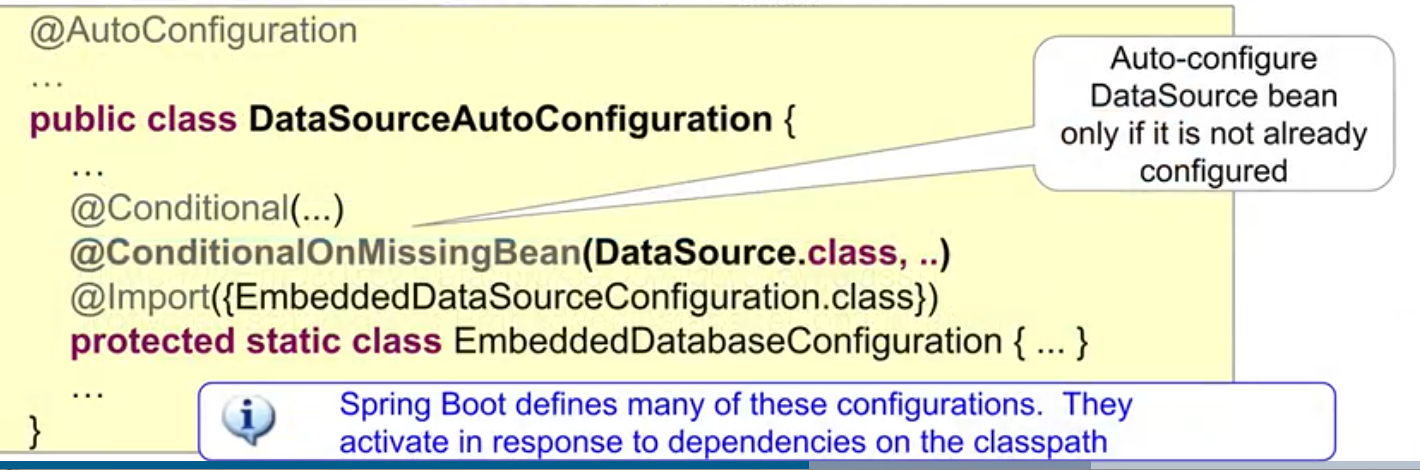
\includegraphics[width=1\linewidth]{datasourceautoconfiguration}
    \caption{Spring's DataSourceAutoConfiguration class.}
    \label{fig:datasourceautoconfiguration}
\end{figure}

\subsection{Testing with Spring Boot}

Test support is provided by two modules: spring-boot-test contains core items, and spring-boot-test-autoconfigure supports auto-configuration for tests.

spring-boot-starter-test imports both Spring Boot test modules as well as JUnit Jupiter, AssertJ, Hamcrest, and a number of other useful libraries. Precisely:

\begin{itemize}
    \item JUnit 5: The de-facto standard for unit testing Java applications.

    \item Spring Test and Spring Boot Test: Utilities and integration test support for Spring Boot applications.

    \item AssertJ: A fluent assertion library.

    \item Hamcrest: A library of matcher objects (also known as constraints or predicates).

    \item Mockito: A Java mocking framework.

    \item JSONassert: An assertion library for JSON.

    \item JsonPath: XPath for JSON.

    \item Awaitility: A library for testing asynchronous systems.

\end{itemize}

\subsection{Test Configuration}

In Spring testing in general, we use \lstinline|@ContextConfiguration(classes=...)| in order to specify which Spring @Configuration to load.
When testing Spring Boot applications, this is often not required. Spring Boot’s @*Test annotations search for the primary configuration automatically.

The search algorithm works up from the package that contains the test until it finds a class annotated with @SpringBootApplication or @SpringBootConfiguration.

To customize the primary configuration, one can use a \textit{nested} \lstinline|@TestConfiguration| class. Unlike a nested @Configuration class, which would be used instead of the application’s primary configuration, a nested @TestConfiguration class is used \textit{in addition to the primary configuration}.

@TestConfiguration can also be used on an \textit{inner} class of a test or the \textit{top-level} class to customize the primary configuration. Doing so indicates that the class should not be picked up by scanning. You can then import the class explicitly where it is required, as shown in the following example:

\begin{lstlisting}
    import org.junit.jupiter.api.Test;

    import org.springframework.boot.test.context.SpringBootTest;
    import org.springframework.context.annotation.Import;

    @SpringBootTest
    @Import(MyTestsConfiguration.class)
    class MyTests {

        @Test
        void exampleTest() {
            // ...
        }

    }
\end{lstlisting}

Note: An imported @TestConfiguration is processed earlier than an inner-class @TestConfiguration and an imported @TestConfiguration will be processed before any configuration found through component scanning.

\subsection{The @SpringBootTest annotation}

The @SpringBootTest annotation is used to specify the main class that should be used when launching an application context for integration tests.

By default, @SpringBootTest does not start a server but instead sets up a mock environment for testing web endpoints.

With Spring MVC, we can query our web endpoints using MockMvc or WebTestClient, as shown in the following example:

\begin{lstlisting}
    @SpringBootTest
    @AutoConfigureMockMvc
    class MyMockMvcTests {

        @Test
        void testWithMockMvc(@Autowired MockMvc mvc) throws Exception {
            mvc.perform(get("/")).andExpect(status().isOk()).andExpect(content().string("Hello World"));
        }

        // If Spring WebFlux is on the classpath, you can drive MVC tests with a WebTestClient
        @Test
        void testWithWebTestClient(@Autowired WebTestClient webClient) {
            webClient
            .get().uri("/")
            .exchange()
            .expectStatus().isOk()
            .expectBody(String.class).isEqualTo("Hello World");
        }

    }

\end{lstlisting}

By default, @SpringBootTest will not start a server. You can use the webEnvironment attribute of @SpringBootTest to further refine how your tests run:

\begin{itemize}
    \item MOCK(Default) : Loads a web ApplicationContext and provides a mock web environment. Embedded servers are not started when using this annotation. If a web environment is not available on your classpath, this mode transparently falls back to creating a regular non-web ApplicationContext. It can be used in conjunction with @AutoConfigureMockMvc or @AutoConfigureWebTestClient for mock-based testing of your web application.

    \item RANDOM\_PORT: Loads a WebServerApplicationContext and provides a real web environment. Embedded servers are started and listen on a random port.
    Alternatively, the property \lstinline|server.port| may be set to 0.
    The @LocalServerPort annotation can be used to inject the \textit{actual port used} into your test.

    \item DEFINED\_PORT: Loads a WebServerApplicationContext and provides a real web environment. Embedded servers are started and listen on a defined port (from your application.properties) or on the default port of 8080.

    \item NONE: Loads an ApplicationContext by using SpringApplication but does not provide any web environment (mock or otherwise).
\end{itemize}

\subsection{Auto-configured Spring MVC Tests: @WebMvcTest}

To test whether Spring MVC controllers are working as expected, use the @WebMvcTest annotation.

@WebMvcTest auto-configures the Spring MVC infrastructure and limits scanned beans to @Controller, @ControllerAdvice, @JsonComponent, Converter, GenericConverter, Filter, HandlerInterceptor, WebMvcConfigurer, WebMvcRegistrations, and HandlerMethodArgumentResolver.

Auto-configured capabilities include: a templating engine (Thymeleaf), Jackson, caching.

Regular @Component and @ConfigurationProperties beans are not scanned when the @WebMvcTest annotation is used. @EnableConfigurationProperti es can be used to include @ConfigurationProperties beans.

Often, @WebMvcTest is limited to a single controller and is used in combination with @MockBean to provide mock implementations for required collaborators.

@WebMvcTest also auto-configures \lstinline|MockMvc|.


\subsection{Auto-Configuration for Slice Tests}
\subsubsection{Auto-configured JPA Tests}

The annotation \lstinline|@DataJpaTest| causes the following auto-configuration to take place:

\begin{lstlisting}
    // optional:org.springframework.boot.testcontainers.
       service.connection.ServiceConnectionAutoConfiguration

    // org.springframework.boot.autoconfigure.
       cache.CacheAutoConfiguration

       data.jpa.JpaRepositoriesAutoConfiguration

       flyway.FlywayAutoConfiguration
       jdbc.DataSourceAutoConfiguration jdbc.DataSourceTransactionManagerAutoConfiguration jdbc.JdbcClientAutoConfiguration jdbc.JdbcTemplateAutoConfiguration liquibase.LiquibaseAutoConfiguration

        orm.jpa.HibernateJpaAutoConfiguration sql.init.SqlInitializationAutoConfiguration TransactionAutoConfiguration

        //org.springframework.boot.test.
        autoconfigure.jdbc.TestDatabaseAutoConfiguration autoconfigure.orm.jpa.TestEntityManagerAutoConfiguration

\end{lstlisting}

Note especially the auto-configuration of caching, JDBCTemplate, Liquibase and Flyway.

\subsection{TestRestTemplate}

Spring Boot also includes a TestRestTemplate that is useful in integration tests. You can get a vanilla template or one that sends Basic HTTP authentication (with a username and password). In either case, the template is fault tolerant. This means that it behaves in a test-friendly way by not throwing exceptions on 4xx and 5xx errors. Instead, such errors can be detected through the returned ResponseEntity and its status code.

TestRestTemplate can be instantiated directly in your integration tests:

\begin{lstlisting}
    import org.junit.jupiter.api.Test;

    import org.springframework.boot.test.web.client.
    TestRestTemplate;
    import org.springframework.http.ResponseEntity;

    import static org.assertj.core.api.Assertions.assertThat;

    class MyTests {

        private final TestRestTemplate template = new TestRestTemplate();

        @Test
        void testRequest() {
            ResponseEntity<String> headers = this.template.getForEntity(
                "https://myhost.example.com/example", String.class);
            assertThat(
            headers.getHeaders().getLocation()).hasHost(
                "other.example.com");
        }
    }
\end{lstlisting}

Alternatively, if you use the \lstinline|@SpringBootTest| annotation with WebEnvironment.RANDOM\_PORT or WebEnvironment.DEFINED\_PORT, you can inject a fully configured TestRestTemplate and start using it. If necessary, additional customizations can be applied through the RestTemplateBuilder bean. Any URLs that do not specify a host and port automatically connect to the embedded server:

\begin{lstlisting}
import java.time.Duration;

import org.junit.jupiter.api.Test;

import org.springframework.beans.factory.annotation.Autowired;
import org.springframework.boot.test.context.SpringBootTest;
import org.springframework.boot.test.context.SpringBootTest.
    WebEnvironment;
import org.springframework.boot.test.context.TestConfiguration;
import org.springframework.boot.test.web.client.TestRestTemplate;
import org.springframework.boot.web.client.RestTemplateBuilder;
import org.springframework.context.annotation.Bean;
import org.springframework.http.HttpHeaders;

import static org.assertj.core.api.Assertions.assertThat;

@SpringBootTest(webEnvironment = WebEnvironment.RANDOM_PORT)
class MySpringBootTests {

    @Autowired
    private TestRestTemplate template;

    @Test
    void testRequest() {
        HttpHeaders headers = this.template.getForEntity("/example", String.class).getHeaders();
        assertThat(headers.getLocation())
            .hasHost("other.example.com");
    }

    @TestConfiguration(proxyBeanMethods = false)
    static class RestTemplateBuilderConfiguration {

        @Bean
        RestTemplateBuilder restTemplateBuilder() {
            return new RestTemplateBuilder().setConnectTimeout(
                Duration.ofSeconds(1))
            .setReadTimeout(Duration.ofSeconds(1));
        }

    }

}
\end{lstlisting}


\subsection{Spring Boot Actuator}

The recommended way to enable the features is to add a dependency on the spring-boot-starter-actuator starter.

\subsubsection{Endpoints}

Actuator endpoints let you monitor and interact with your application. Spring Boot includes a number of built-in endpoints and lets you add your own. For example, the health endpoint provides basic application health information.

You can enable or disable each individual endpoint and expose them (make them remotely accessible) over HTTP or JMX. An endpoint is considered to be available when it is \textit{both enabled and exposed}.

The built-in endpoints are auto-configured only when they are available. Most applications choose exposure over HTTP, where the ID of the endpoint and a prefix of /actuator is mapped to a URL. For example, by default, the health endpoint is mapped to /actuator/health.

By default, \textit{all endpoints except for shutdown are enabled}. To configure the enablement of an endpoint, use its management.endpoint.\textless id\textgreater.enabled property. The following example enables the shutdown endpoint:

\begin{lstlisting}
   management.endpoint.shutdown.enabled=true
\end{lstlisting}

If you prefer endpoint enablement to be opt-in rather than opt-out, set the \lstinline|management.endpoints.enabled-by-default| property (which by default is true) to false and use individual endpoint enabled properties to opt back in. The following example enables the info endpoint and disables all other endpoints:

\begin{lstlisting}
    management.endpoints.enabled-by-default=false
    management.endpoint.info.enabled=true
\end{lstlisting}

Disabled endpoints are removed entirely from the application context. If you want to change only the technologies over which an endpoint is exposed, use the include and exclude properties instead.

By default, only the health endpoint is \textit{exposed} over HTTP and JMX.

To change which endpoints are exposed, use the following technology-specific include and exclude properties: management.endpoints.jmx.exposure.exclude,
management.endpoints.jmx.exposure.include; management.endpoints.web.exposure.exclude, management.endpoints.web.exposure.include.

The include property lists the IDs of the endpoints that are exposed. The exclude property lists the IDs of the endpoints that should not be exposed. The exclude property takes precedence over the include property. You can configure both the include and the exclude properties with a list of endpoint IDs.

For example, to only expose the health and info endpoints over JMX, use the following property:

\begin{lstlisting}
    management.endpoints.jmx.exposure.include=health,info
\end{lstlisting}

* can be used to select all endpoints. For example, to expose everything over HTTP except the env and beans endpoints, use the following properties:

\begin{lstlisting}
    management.endpoints.web.exposure.include=*
    management.endpoints.web.exposure.exclude=env,beans

\end{lstlisting}

\paragraph{Monitoring and Management Over HTTP}

Customization:

\begin{lstlisting}
    // base for all endpoints
    management.endpoints.web.base-path=

    // for a specific endpoint
    management.endpoints.web.path-mapping.<actuator>
    // e.g.
    management.endpoints.web.path-mapping.health=custom-health

    // prt
    management.server.port=8081
\end{lstlisting}



\paragraph{Health information}

Information exposed by the health endpoint depends on the \lstinline|management.endpoint.health.show-details| and \lstinline|management.endpoint.health.show-components| properties, which can be configured with one of the following values: never, when-authorized, always
.

The default value is never. A user is considered to be authorized when they are in one or more of the endpoint’s roles. If the endpoint has no configured roles (the default), all authenticated users are considered to be authorized. You can configure the roles by using the management.endpoint.health.roles property.

Health information is collected from the content of a HealthContributorRegistry (by default, all HealthContributor instances defined in your ApplicationContext). Spring Boot includes a number of auto-configured HealthContributors, and you can also write your own.

A \lstinline|HealthContributor| can be either a \lstinline|HealthIndicator| or a \lstinline|CompositeHealthContributor|.

By default, the final system health is derived by a StatusAggregator, which sorts the statuses from each HealthIndicator based on an ordered list of statuses. The first status in the sorted list is used as the overall health status. If no HealthIndicator returns a status that is known to the StatusAggregator, an UNKNOWN status is used.

\paragraph{Auto-configured HealthIndicators}

\begin{lstlisting}
    cassandra
    couchbase
    db
    diskspace
    elasticsearch
    hazelcast
    influxdb
    jms
    ldap
    mail
    mongo
    neo4j
    ping
    rabbit
    redis
\end{lstlisting}

\paragraph{Writing Custom HealthIndicators}

To provide custom health information, you can register Spring beans that implement the HealthIndicator interface. You need to provide an implementation of the \lstinline|health()| method and return a \lstinline|Health| response. The Health response should include a status and can optionally include additional details to be displayed. The following code shows a sample HealthIndicator implementation:

    \begin{lstlisting}
    import org.springframework.boot.actuate.health.Health;
    import org.springframework.boot.actuate.health.HealthIndicator;
    import org.springframework.stereotype.Component;

    @Component
    public class MyHealthIndicator implements HealthIndicator {

        @Override
        public Health health() {
            int errorCode = check();
            if (errorCode != 0) {
                return Health.down().withDetail("Error Code", errorCode).build();
            }
            return Health.up().build();
        }

        private int check() {
            // perform some specific health check
            return ...
        }

    }
    \end{lstlisting}

The identifier for a given HealthIndicator is the name of the bean without the HealthIndicator suffix, if it exists. In the preceding example, the health information is available in an entry named my.

\paragraph{Info Endpoint: Application Information}

Application information exposes various information collected from all \lstinline|InfoContributor| beans defined in your ApplicationContext. Spring Boot includes a number of auto-configured InfoContributor beans, and you can write your own.

Auto-configured InfoContributors may be:

\begin{lstlisting}
    // if there's a META-INF/build-info.properties resource
    build
    //  Exposes any property from the Environment whose name starts with info
    env
    // git.properties resource exists
    git
    java
    os
    process
\end{lstlisting}

Whether an individual contributor is enabled is controlled by its management.info.someid.enabled property.

Different contributors have different defaults for this property, depending on their prerequisites and the nature of the information that they expose.

With no prerequisites to indicate that they should be enabled, the env, java, os, and process contributors are disabled by default.

The build and git info contributors are enabled by default.

The Health Indicator status severity order be changed using the \lstinline|management.health.status.order| property.

\paragraph{Custom Application Information}

When the env contributor is enabled, you can customize the data exposed by the info endpoint by setting info.* Spring properties. \textit{All Environment properties under the info key are automatically exposed.} For example, you could add the following settings to your application.properties file:

    \begin{lstlisting}
    info.app.encoding=UTF-8
    info.app.java.source=17
    info.app.java.target=17

    \end{lstlisting}

\paragraph{Writing Custom InfoContributors}

    To provide custom application information, you can register Spring beans that implement the InfoContributor interface.

\begin{lstlisting}
    import java.util.Collections;

    import org.springframework.boot.actuate.info.Info;
    import org.springframework.boot.actuate.info.InfoContributor;
    import org.springframework.stereotype.Component;

    @Component
    public class MyInfoContributor implements InfoContributor {

        @Override
        public void contribute(Info.Builder builder) {
            builder.withDetail("example", Collections.singletonMap("key", "value"));
        }

    }
\end{lstlisting}

\paragraph{Tracing}

Spring Boot Actuator provides dependency management and auto-configuration for Micrometer Tracing, a facade for popular tracer libraries.

Spring Boot ships auto-configuration for the following tracers:

\begin{itemize}
    \item OpenTelemetry with Zipkin, Wavefront, or OTLP
    \item OpenZipkin Brave with Zipkin or Wavefront
\end{itemize}

\paragraph{Recording HTTP Exchanges}

You can enable recording of HTTP exchanges by providing a bean of type \lstinline|HttpExchangeRepository| in your application’s configuration. For convenience, Spring Boot offers \lstinline|InMemoryHttpExchangeRepository|, which, by default, stores the last 100 request-response exchanges.

You can use the httpexchanges endpoint to obtain information about the request-response exchanges that are stored in the HttpExchangeRepository.

To customize the items that are included in each recorded exchange, use the \lstinline|management.httpexchanges.recording.include| configuration property.

To disable recoding entirely, set \lstinline|management.httpexchanges.recording.enabled| to false.

\paragraph{Auditing}

Once Spring Security is in play, Spring Boot Actuator has a flexible audit framework that publishes events (by default, “authentication success”, “failure” and “access denied” exceptions). This feature can be very useful for reporting and for implementing a lock-out policy based on authentication failures.

You can enable auditing by providing a bean of type \lstinline|AuditEventRepository| in your application’s configuration. For convenience, Spring Boot offers an \lstinline|InMemoryAuditEventRepository|.

To customize published security events, you can provide your own implementations of \lstinline|AbstractAuthenticationAuditListener| and \lstinline|AbstractAuthorizationAuditListener|.

You can also use the audit services for your own business events. To do so, either inject the \lstinline|AuditEventRepository| bean into your own components and use that directly or publish an \lstinline|AuditApplicationEvent| with the Spring \lstinline|ApplicationEventPublisher| (by implementing \lstinline|ApplicationEventPublisherAware|).


\end{document}




























